% Options for packages loaded elsewhere
% Options for packages loaded elsewhere
\PassOptionsToPackage{unicode}{hyperref}
\PassOptionsToPackage{hyphens}{url}
\PassOptionsToPackage{dvipsnames,svgnames,x11names}{xcolor}
%
\documentclass[
  11pt,
  letterpaper,
]{scrartcl}
\usepackage{xcolor}
\usepackage[inner=3cm,outer=3cm,top=3cm,bottom=3cm,headsep=22pt,headheight=11pt,footskip=33pt,ignorehead,ignorefoot,heightrounded]{geometry}
\usepackage{amsmath,amssymb}
\setcounter{secnumdepth}{5}
\usepackage{iftex}
\ifPDFTeX
  \usepackage[T1]{fontenc}
  \usepackage[utf8]{inputenc}
  \usepackage{textcomp} % provide euro and other symbols
\else % if luatex or xetex
  \usepackage{unicode-math} % this also loads fontspec
  \defaultfontfeatures{Scale=MatchLowercase}
  \defaultfontfeatures[\rmfamily]{Ligatures=TeX,Scale=1}
\fi
\usepackage{lmodern}
\ifPDFTeX\else
  % xetex/luatex font selection
  \setmonofont[Scale=0.7]{DejaVu Sans Mono}
\fi
% Use upquote if available, for straight quotes in verbatim environments
\IfFileExists{upquote.sty}{\usepackage{upquote}}{}
\IfFileExists{microtype.sty}{% use microtype if available
  \usepackage[]{microtype}
  \UseMicrotypeSet[protrusion]{basicmath} % disable protrusion for tt fonts
}{}
\usepackage{setspace}
% Make \paragraph and \subparagraph free-standing
\makeatletter
\ifx\paragraph\undefined\else
  \let\oldparagraph\paragraph
  \renewcommand{\paragraph}{
    \@ifstar
      \xxxParagraphStar
      \xxxParagraphNoStar
  }
  \newcommand{\xxxParagraphStar}[1]{\oldparagraph*{#1}\mbox{}}
  \newcommand{\xxxParagraphNoStar}[1]{\oldparagraph{#1}\mbox{}}
\fi
\ifx\subparagraph\undefined\else
  \let\oldsubparagraph\subparagraph
  \renewcommand{\subparagraph}{
    \@ifstar
      \xxxSubParagraphStar
      \xxxSubParagraphNoStar
  }
  \newcommand{\xxxSubParagraphStar}[1]{\oldsubparagraph*{#1}\mbox{}}
  \newcommand{\xxxSubParagraphNoStar}[1]{\oldsubparagraph{#1}\mbox{}}
\fi
\makeatother


\usepackage{longtable,booktabs,array}
\newcounter{none} % for unnumbered tables
\usepackage{calc} % for calculating minipage widths
% Correct order of tables after \paragraph or \subparagraph
\usepackage{etoolbox}
\makeatletter
\patchcmd\longtable{\par}{\if@noskipsec\mbox{}\fi\par}{}{}
\makeatother
% Allow footnotes in longtable head/foot
\IfFileExists{footnotehyper.sty}{\usepackage{footnotehyper}}{\usepackage{footnote}}
\makesavenoteenv{longtable}
\usepackage{graphicx}
\makeatletter
\newsavebox\pandoc@box
\newcommand*\pandocbounded[1]{% scales image to fit in text height/width
  \sbox\pandoc@box{#1}%
  \Gscale@div\@tempa{\textheight}{\dimexpr\ht\pandoc@box+\dp\pandoc@box\relax}%
  \Gscale@div\@tempb{\linewidth}{\wd\pandoc@box}%
  \ifdim\@tempb\p@<\@tempa\p@\let\@tempa\@tempb\fi% select the smaller of both
  \ifdim\@tempa\p@<\p@\scalebox{\@tempa}{\usebox\pandoc@box}%
  \else\usebox{\pandoc@box}%
  \fi%
}
% Set default figure placement to htbp
\def\fps@figure{htbp}
\makeatother





\setlength{\emergencystretch}{3em} % prevent overfull lines

\providecommand{\tightlist}{%
  \setlength{\itemsep}{0pt}\setlength{\parskip}{0pt}}




\usepackage[]{natbib}
\bibliographystyle{econometrica}


\setkomafont{disposition}{\rmfamily\bfseries}
\usepackage{url}
\usepackage[noblocks]{authblk}
\renewcommand*{\Authsep}{, }
\renewcommand*{\Authand}{, }
\renewcommand*{\Authands}{, }
\renewcommand\Affilfont{\small}
\makeatletter
\@ifpackageloaded{caption}{}{\usepackage{caption}}
\AtBeginDocument{%
\ifdefined\contentsname
  \renewcommand*\contentsname{Table of contents}
\else
  \newcommand\contentsname{Table of contents}
\fi
\ifdefined\listfigurename
  \renewcommand*\listfigurename{List of Figures}
\else
  \newcommand\listfigurename{List of Figures}
\fi
\ifdefined\listtablename
  \renewcommand*\listtablename{List of Tables}
\else
  \newcommand\listtablename{List of Tables}
\fi
\ifdefined\figurename
  \renewcommand*\figurename{Figure}
\else
  \newcommand\figurename{Figure}
\fi
\ifdefined\tablename
  \renewcommand*\tablename{Table}
\else
  \newcommand\tablename{Table}
\fi
}
\@ifpackageloaded{float}{}{\usepackage{float}}
\floatstyle{ruled}
\@ifundefined{c@chapter}{\newfloat{codelisting}{h}{lop}}{\newfloat{codelisting}{h}{lop}[chapter]}
\floatname{codelisting}{Listing}
\newcommand*\listoflistings{\listof{codelisting}{List of Listings}}
\makeatother
\makeatletter
\makeatother
\makeatletter
\@ifpackageloaded{caption}{}{\usepackage{caption}}
\@ifpackageloaded{subcaption}{}{\usepackage{subcaption}}
\makeatother
\usepackage{bookmark}
\IfFileExists{xurl.sty}{\usepackage{xurl}}{} % add URL line breaks if available
\urlstyle{same}
% fallback for those not using the hyperref driver hyperxmp:
\makeatletter
\@ifundefined{xmpquote}{\newcommand{\xmpquote}[1]{#1}}{}
\makeatother
\hypersetup{
  pdftitle={Capacity{,} Training{,} and Default in the Race to Artificial General Intelligence},
  pdfkeywords={\xmpquote{real options}, \xmpquote{irreversible capacity
investment}, \xmpquote{artificial intelligence}, \xmpquote{duopoly
preemption}, \xmpquote{default risk}},
  colorlinks=true,
  linkcolor={blue},
  filecolor={Maroon},
  citecolor={Blue},
  urlcolor={Blue},
  pdfcreator={LaTeX via pandoc}}


\title{Capacity, Training, and Default in the Race to Artificial General
Intelligence\thanks{I thank Armand Jr Brunelle, Tolga Cenesizoglu,
Joshua Gans, Charles Martineau, and Piotr Orłowski for helpful comments.
AI assistance was used extensively in writing this paper; the code for
the project and details on the use of AI tools are available at
\url{https://github.com/fintech-research/ai-lab-investment}. Vincent
Grégoire: HEC Montréal (vincent.gregoire@hec.ca).}}
\author[1]{Vincent Grégoire}
\affil[1]{HEC Montréal}
\date{September 10, 2026}

\begin{document}
\maketitle
\begin{abstract}
Frontier AI laboratories must decide how much irreversible capacity to
build under uncertain arrival of Artificial General Intelligence (AGI),
and how to split it between inference (current revenue) and training
(future capability). I develop a real-options model with regime
switching, duopoly competition, endogenous default, and diminishing
returns to capacity whose curvature is motivated by AI scaling laws.
Under a stated pricing convention the model yields analytical investment
triggers and a semi-analytical preemption equilibrium in which
competition compresses investment timing, while beliefs about AI
timelines, not competitive position, pin down the training fraction. It
also produces ``faith-based survival'': at the optimal allocation,
optimism about the switch raises the post-AGI continuation value and
lowers the default boundary, though creditors cannot recover that value
in bankruptcy. Calibration to four AI lab archetypes shows how
heterogeneous beliefs about AI timelines can generate cross-sectional
differences in investment. In the calibrated model, conservative
underinvestment is costlier in expected value, but aggressive
overinvestment carries higher tail default risk.
\end{abstract}

% Keywords and JEL classification, displayed on the title page below the abstract.
% The keyword list mirrors the `keywords:` frontmatter in index.qmd and
% index-blind.qmd (which also feed the PDF metadata); JEL codes are maintained
% here. Keep the list at 3--5 entries: Management Science caps keywords at five.
\begin{center}
\begin{minipage}{0.85\textwidth}
\small
\noindent\textbf{Keywords:} real options; irreversible capacity investment; artificial intelligence; duopoly preemption; default risk\par
\medskip
\noindent\textbf{JEL classification:} C73, D25, G31, G32, G33, L13, O33\par
\end{minipage}
\end{center}
\bigskip


\setstretch{1.25}
\section{Introduction}\label{sec-introduction}

The race to build artificial intelligence infrastructure commits an
unusually large and concentrated pool of capital: combined capital
expenditure by the leading AI laboratories and their compute partners is
projected to reach \$660--690 billion in 2026,\footnote{Sources: Amazon
  FY2026 capital-expenditure guidance (CNBC, February 5, 2026); Alphabet
  Q4 2025 earnings release (SEC EDGAR, exhibit 99.1); Microsoft FY2026
  Q2 earnings release.} and OpenAI's Stargate joint venture alone
commits up to \$500 billion in U.S. AI infrastructure through
2029.\footnote{\url{https://openai.com/index/announcing-the-stargate-project/}.}
These investments are largely irreversible, and whether and when AI
capabilities will reach a transformative threshold, the uncertainty that
drives them, remains unresolved. This paper asks how a firm should time,
size, and allocate an irreversible capacity investment when the return
to that capacity depends on a regime change whose arrival is uncertain
and whose competitive consequences depend on how the capacity was used
beforehand.

The allocation margin is what makes the problem distinctive. A frontier
AI laboratory produces intelligence by combining two forms of compute
drawn from the same scarce hardware: \emph{training compute}, which
optimizes a neural network's parameters on massive datasets and yields a
model whose quality scales as a power law of compute invested
\citep{kaplan2020scaling, altman2025observations}, and \emph{inference
compute}, which runs the trained model to serve predictions and generate
revenue. The same asset can either produce revenue now or build the
capability that determines the firm's position in a future that may not
arrive. Allocating capacity toward future capability can support
continuation value while eroding the liquidation collateral creditors
can seize, and that distinction disciplines how timeline beliefs affect
distress. A firm that bets on the future by allocating capacity to
training weakens its ability to survive to that future, so the option to
grow and the risk of failure are linked through a single decision.

Firms must commit this capital under widely different priors about the
same event. The prize is Artificial General Intelligence (AGI): a step
change in model capability sufficient to automate a broad range of
cognitive tasks and generate sustained, qualitatively higher demand for
compute \citep{amodei2024machines}. Executive forecasts of its arrival
run from ``superintelligence in a few thousand days''
\citep{altman2024intelligence} and 2026--2027
\citep{amodei2024machines}, through ``AGI in 2026,''\footnote{Elon Musk,
  post on X, 2025:
  \url{https://x.com/elonmusk/status/2025124840806514916}.} to ``not
with current architectures.''\footnote{PYMNTS, ``Meta: Large Language
  Models Will Not Get to Human-Level Intelligence,'' 2025.}

Existing frameworks illuminate parts of this problem but not its core
difficulty. Real-options models
\citep{mcdonald1986value, dixit1994investment} characterize
irreversibility and timing but take the use of installed capacity as
given; R\&D race models \citep{loury1979market, reinganum1982strategic}
treat pre-breakthrough expenditure as pure cost with no concurrent
revenue; structural credit models \citep{leland1994corporate}, including
the branch that embeds regime switching, take the size of the growth
option as exogenous rather than as a capacity-allocation choice.

I therefore develop a model in which a firm chooses when to invest, how
much capacity to install, and what fraction \(\phi\) to devote to
training versus inference, facing regime-switching demand
\citep{guo2005investment}, duopoly preemption
\citep{grenadier2002option, huisman2015strategic}, endogenous default
\citep{leland1994corporate}, and diminishing returns to capacity, with
the curvature parameter motivated by empirical scaling laws
\citep{kaplan2020scaling, hoffmann2022training}. In regime \(L\), the
current low-demand regime, revenue depends on inference capacity through
a Tullock contest, in which a firm's contest share is its inference
capacity's share of the industry total, each raised to the power
\(\alpha\); in regime \(H\), the post-AGI regime, it depends on training
quality. Duopoly is the minimal setting that captures preemption,
allocation incentives, and leverage.

The paper makes three contributions. First, I characterize the optimal
training fraction, investment trigger, and capacity analytically, under
a pricing convention for the pre-investment option that
Section~\ref{sec-model} states and Internet Appendix B benchmarks
against the unrestricted stopping problem. Preemption operates on the
timing margin: at baseline volatility, and conditional on the convention
that the leader installs the monopoly-phase optimal scale, the leader
invests at a trigger roughly 43\% below the monopoly benchmark. It does
not operate on the allocation margin: the contest shares cancel from the
allocation first-order condition, so leader, follower, and monopolist
choose the same training fraction.

Second, I identify \emph{faith-based survival}, an
optimism-through-allocation channel: over the arrival rates the
calibration considers, a firm that expects the switch sooner trains
more, and at its optimal allocation the higher arrival rate raises the
effective revenue coefficient \(A_{\text{eff}}\) through the expected
post-AGI continuation value, lowering the default boundary (at a fixed
belief, the boundary is U-shaped in the training fraction, so training
beyond the optimum raises it). The same allocation raises the loss given
default, because a larger training fraction shrinks the inference
business creditors can liquidate, and creditors cannot recover the
continuation value in bankruptcy. The survival channel operates only
where it dominates current cash-flow weakness, a condition I
characterize in closed form for the symmetric duopoly.

Third, I quantify \emph{Dario's dilemma}, the loss a firm incurs by
investing on a belief about the AGI arrival intensity \(\lambda\) that
differs from its true value. In the single-firm reduced model, capacity
does not depend on the belief, so the mistakes run through timing and
allocation: a pessimistic firm invests too late, under-allocates to
training, and forgoes much of the post-AGI option value, while an
optimistic firm invests too early, over-allocates, and sacrifices the
inference revenue it needs to survive. Anthropic CEO Dario Amodei
describes the overbuilding side: ``I could buy \$1 trillion of compute
that starts at the end of 2027\ldots{} there's no hedge on Earth that
could stop me from going bankrupt'' \citep{amodei2026dwarkesh}. In a
stylized calibration to four AI lab archetypes, the asymmetry can be
substantial (Numerical Finding 1): investing as though
\(\lambda = 0.02\) when the true intensity is \(0.10\) costs roughly
26\% of firm value, against about 6\% for \(\lambda = 0.20\). The
dilemma is nonetheless two-sided, because overinvestment concentrates
risk in the tail: at \(\lambda_{\text{invest}} = 0.50\) and leverage
\(\ell = 0.40\), the five-year default probability (a no-switch upper
bound) is nearly eight times its value under correct beliefs.

\subsection{Related literature}\label{sec-literature}

The real-options foundation rests on \citet{mcdonald1986value} for
optimal timing of irreversible investment and
\citet{pindyck1988irreversible} for capacity choice.
\citet{guo2005investment} model demand with regime-dependent drift and
volatility, showing large investment jumps on favorable regime arrival;
\citet{decamps2006irreversible} study the choice between two
irreversible projects of different scale under a single geometric
Brownian output price, with an extension in which the firm may later
switch from the smaller to the larger project; the present paper's scale
choice is in that tradition, while its \(L \to H\) transition is an
exogenous Poisson regime switch rather than a project switch chosen by
the firm. Neither includes strategic interaction, training-inference
allocation, or default risk. The capacity-choice problem is also studied
in operations management \citep{vanmieghem2003capacity}, whose closest
construct is resource flexibility: \citet{chod2005resource} show that a
flexible resource allocated across products \emph{after} demand is
observed substitutes for capacity. Compute is flexible in that sense,
but the allocation here is a commitment made at installation whose
training component pays off only in a different demand regime, and it is
priced jointly with the firm's default decision.

Strategic real-options models replace the single decision maker with
rivals whose entry erodes the option value of waiting
\citep{grenadier2002option}. The closest strategic-investment paper is
\citet{huisman2015strategic}, who study a duopoly with joint timing and
capacity choice; I extend their framework with endogenous default risk,
training-inference allocation, diminishing returns, and regime
switching. \citet{aguerrevere2003equilibrium} and
\citet{aguerrevere2009real} link installed capacity and competitive
intensity to the composition of firm value between assets in place and
growth options, and hence to expected returns, an antecedent of the
training-beta conjecture of Section~\ref{sec-discussion}; here the risk
composition shifts with the \emph{split} of a given capacity rather than
with its level. \citet{lambrecht2003real} study duopoly real options
under incomplete information, where firms hold private signals about the
payoff, related to the heterogeneous beliefs about the AGI arrival rate
\(\lambda\) here but without the allocation or default mechanisms.

The paper also connects to patent races and R\&D competition.
\citet{loury1979market} and \citet{reinganum1982strategic} model firms
choosing R\&D intensity to accelerate a stochastic Poisson breakthrough,
and \citet{harris1987racing} derive a discouragement effect for lagging
firms that echoes the follower's delayed entry in the duopoly
equilibrium; in the present model the \emph{allocation} margin is immune
to this discouragement (Proposition 3(ii)), so position affects when
firms invest, not how they split capacity. The key departure is the dual
role of capacity: in standard races, investment during the race is pure
cost, whereas here installed capacity generates inference revenue before
AGI arrives and training quality determines position afterwards.

The firm's default decision follows the structural credit-risk tradition
of \citet{merton1974pricing} and \citet{leland1994corporate}, a
literature that already embeds regime switching in the Leland framework.
\citet{hackbarth2006capital} let cash flows depend on a two-state
macroeconomic regime and derive default and financing policies that
adapt to the cycle; \citet{chen2010macroeconomic} and
\citet{bhamra2010levered} add a consumption-based pricing kernel.
Proposition 2 is therefore not the first default boundary derived in a
regime-switching environment; those papers in fact solve the fully
coupled system with regime-contingent boundaries, whereas
Equation~\ref{eq-default-boundary} uses a single boundary that embeds
the switch in unconditional expectation (Section~\ref{sec-model}
documents the resulting approximation error). The Leland framework suits
public-debt issuers; for the VC-backed archetypes in the calibration,
``default'' should be read broadly as financial distress (failed funding
round, liquidity crisis), consistent with \citet{gornall2020squaring}.

The model's technology assumptions come from the economics of AI.
Training exhibits power-law scaling
\citep{kaplan2020scaling, hoffmann2022training}, motivating the concave
production function, and \citet{agrawal2019economics} frame AI as a
prediction technology connecting inference demand to value creation.
\citet{aghion2019artificial}, \citet{acemoglu2024simple},
\citet{korinek2024scenarios}, and \citet{jones2024agi} analyze the
growth implications of transformative AI in general equilibrium; the
present paper is partial equilibrium and complements them with a
firm-level investment and allocation problem. On the allocation margin
itself, the closest analog is \citet{akcigit2018growth} on exploitation
versus exploration R\&D, set in a multi-product firm rather than in a
compute allocation problem.

The marginal contribution is a result the closest models do not
generate. In the papers that combine irreversible investment with
endogenous default \citep{kumar2018optimal, hackbarth2014capital},
installed capital is homogeneous, so no single decision variable moves
the default boundary and the liquidation collateral in opposite
directions. The training fraction \(\phi\) does exactly that here: below
the allocation optimum, raising it lowers the default boundary through
the expected post-AGI continuation value (\emph{faith-based survival},
whose belief-side thresholds are \textbf{?@eq-phi-underbar} and
\textbf{?@eq-phi-tilde}), while shrinking the inference business
creditors can liquidate, so the value that keeps the firm alive is
worthless in bankruptcy. That opposition is what makes belief errors
asymmetric in \emph{Dario's dilemma}, with optimism acting through the
training allocation to lower the default boundary while leverage
concentrates tail risk on the aggressive side. The regime-switching
credit models take the size of the growth option as exogenous, so the
firm cannot buy survival by sacrificing current revenue, and the
allocation problems closest in structure
\citep{akcigit2018growth, chod2005resource} are solved for firms whose
survival is not at stake. The investment-financing framework follows
\citet{hackbarth2012corporate}; Internet Appendix I collects additional
antecedents and the empirical motivation for the duopoly setting.

The paper proceeds as follows. Section~\ref{sec-model} presents the
model environment, the single-firm benchmark, and the duopoly
equilibrium with default risk, and contains the analytical and
semi-analytical results. Section~\ref{sec-calibration} describes the
stylized calibration to frontier AI lab archetypes.
Section~\ref{sec-valuation} develops credit risk and Dario's dilemma,
Section~\ref{sec-discussion} considers policy implications, testable
predictions, and limitations, and Section~\ref{sec-conclusion}
concludes. The Internet Appendix collects the proofs, numerical
verification methods, calibration sources, robustness exercises, and
supporting figures.

\section{The Model}\label{sec-model}

The model has four stages: the demand environment and technology, the
single-firm benchmark, the solution conventions on which the closed
forms rest, and the duopoly with default risk.

\subsection{Environment}\label{environment}

Time is continuous. Demand \(X_t\) governs the revenue available to
frontier AI labs; its units are fixed by the capacity normalization of
Section~\ref{sec-calibration}, so levels below are relative. Demand
follows a geometric Brownian motion with regime-dependent drift and
common volatility:
\begin{equation}\protect\phantomsection\label{eq-gbm}{
dX_t = \mu_s X_t \, dt + \sigma X_t \, dW_t, \quad s \in \{L, H\},
}\end{equation} where \(W_t\) is a standard Brownian motion, \(s\)
indexes the demand regime, and \(\sigma > 0\) is the common volatility
parameter.

The economy starts in the low-demand regime \(L\) and switches to the
high-demand regime \(H\) at an exogenous Poisson rate \(\lambda > 0\), a
breakthrough that permanently shifts demand to a higher trajectory.
Throughout, \(\lambda\) is a parameter of the firm's valuation problem
rather than a measured frequency: a firm holding a shorter AGI timeline
is a firm with a higher \(\lambda\), and every comparative static in
\(\lambda\) should be read that way (Section~\ref{sec-calibration} maps
executive timelines into a range). The high regime is absorbing, which
\emph{assumes} irreversible progress.

I assume \(\mu_H > \mu_L\) and require \(r > \mu_H > \mu_L\) for present
values to be well defined, where \(r\) is the discount rate and
\(\mu_s\) the risk-adjusted growth rate.\footnote{\label{fn:wacc}Following
  \citet[Chapter 4]{dixit1994investment}, valuation uses a single
  \emph{risk-adjusted} (certainty-equivalent) framework: \(r\) is the
  weighted average cost of capital and \(\mu_L\), \(\mu_H\) are growth
  rates \emph{net} of a risk premium. This is \emph{not} a risk-neutral
  pricing measure, so the model's outputs are risk-adjusted objects, not
  market prices. Internet Appendix B states the convention in full.}

\subsection{Technology}\label{technology}

A firm invests an irreversible lump sum \(I(K) = cK^\gamma\) to install
capacity \(K > 0\), where \(\gamma > 1\) captures convex investment
costs: power constraints, GPU supply bottlenecks, and construction
complexity raise the marginal cost of capacity. That AI scaling laws
exhibit diminishing returns to compute
\citep{kaplan2020scaling, hoffmann2022training} is captured separately
by the revenue elasticity \(\alpha \in (0,1)\) below. Capacity is fixed
once installed, in a single lump (Section~\ref{sec-discussion}).

\subsubsection{Training-inference
allocation}\label{training-inference-allocation}

Training and inference compute, defined in
Section~\ref{sec-introduction}, draw on the same scarce hardware. The
allocation problem resembles resource flexibility in operations
management \citep{vanmieghem2003capacity, chod2005resource} but differs
in one respect that matters for valuation: the split is committed at
installation, and its training side pays off only in a regime that has
not yet arrived.

A firm with total installed capacity \(K\) allocates fraction
\(\phi \in [0, 1]\) to training and \(1 - \phi\) to inference, such that
training compute is \(\phi K\) and inference compute is \((1-\phi) K\).
Revenue depends on the demand regime:

\begin{itemize}
\item
  \textbf{Low regime} (\(L\), pre-AGI): revenue derives from
  \emph{inference}, that is, from serving current demand. Firm \(i\)'s
  flow revenue is:
  \begin{equation}\protect\phantomsection\label{eq-revenue-L}{
  \pi_i^L(X) = X \cdot [(1-\phi_i)K_i]^\alpha,
  }\end{equation} where \(\alpha\) is the revenue elasticity of
  capacity.
\item
  \textbf{High regime} (\(H\), post-AGI): revenue derives from
  \emph{training compute}, which I read as a proxy for model capability.
  Firm \(i\)'s flow revenue is:
  \begin{equation}\protect\phantomsection\label{eq-revenue-H}{
  \pi_i^H(X) = X \cdot (\phi_i K_i)^\alpha,
  }\end{equation} with the same elasticity applied to training compute.
\end{itemize}

In regime \(L\) only inference capacity earns revenue, and in regime
\(H\) only training compute does. The knife-edge form is a modelling
device that gives the idle side of the split no revenue at all;
Table~\ref{tbl-domains} records it with the model's other operating
assumptions. The training fraction is fixed at installation, and
Section~\ref{sec-discussion} bounds the resulting bias.

Installed capacity incurs a continuous operating cost at rate
\(\delta > 0\) per unit: power, cooling, maintenance, and
personnel.\footnote{This is distinct from \emph{economic depreciation}:
  \(K\) is constant once installed, and \(\delta K\) is a perpetual flow
  cost, not a decay rate. Section~\ref{sec-calibration} discusses the
  relation to accounting depreciation and to hardware obsolescence
  \citep{deepseek2025r1}.}

Table~\ref{tbl-parameters} and Table~\ref{tbl-notation}, in the
Parameters and Notation section of the Internet Appendix, summarize all
model parameters and key notation; the calibration rationale for each
value is discussed in Section~\ref{sec-calibration}.

\subsection{Single-Firm Benchmark}\label{sec-single-firm}

A single firm holds an option to invest and chooses the trigger \(X^*\),
the capacity \(K^*\), and the training fraction \(\phi^*\) that maximize
its value, under the following conditions.

\textbf{Assumption 1} (Parameter admissibility). \emph{The following
conditions are maintained throughout:}

\emph{(A1) \(r > \mu_H > \mu_L \geq 0\), \(\sigma > 0\),
\(\alpha \in (0,1)\), \(\gamma > 1\), \(c > 0\), \(\delta > 0\),
\(\lambda > 0\).}

\emph{(A2) The option premium condition
\(1/\gamma < (\beta_H - 1)/(\alpha \beta_H) < 1\) holds, ensuring an
interior capacity solution in regime \(H\), where \(\beta_H\) is the
positive root of the H-regime characteristic equation
Equation~\ref{eq-beta-H} below.}

\emph{(A3) The L-regime insufficiency condition
\((1 - 1/\beta_L^+)/\alpha \geq 1\) holds, where \(\beta_L^+\) is the
positive root of the L-regime characteristic equation
\(\tfrac{1}{2}\sigma^2 \beta(\beta - 1) + \mu_L \beta - (r + \lambda) = 0\)
derived below; this is the condition under which the paper adopts the
simplified option value \(F_L \propto X^{\beta_H}\)
(Section~\ref{sec-conventions}). This means that L-regime revenue alone
would not justify investment; the firm may still invest while in regime
\(L\), but only because the combined effective revenue coefficient
\(A_{\text{eff}}\), which includes the H-regime prospect, makes the
investment worthwhile.}

\emph{(A4) \(A_{\text{eff}}(\phi, K)\) is twice continuously
differentiable in \(\phi \in (0,1)\) for fixed \(K > 0\).}

\emph{All four conditions are satisfied at the baseline calibration
(\(\beta_L^+ \approx 3.01\), \((1 - 1/\beta_L^+)/\alpha \approx 1.67\))
and verified computationally at all parameter values used in the paper.
Internet Appendix B provides the full boundary analysis, including
sensitivity of (A2) and (A3) to archetype-specific WACCs and the
treatment when (A3) fails.}

\subsubsection{Installed value}\label{installed-value}

In the absorbing high regime, the value of installed capacity depends on
training compute:
\begin{equation}\protect\phantomsection\label{eq-installed-value-H}{
V_H(X, K, \phi) = \frac{X (\phi K)^\alpha}{r - \mu_H} - \frac{\delta K}{r} = A_H \cdot X \cdot (\phi K)^\alpha - \frac{\delta K}{r},
}\end{equation} where \(A_H = 1/(r - \mu_H)\). In the low regime,
installed value combines current inference revenue and the expected
continuation value from a switch to \(H\):
\begin{equation}\protect\phantomsection\label{eq-installed-value-L}{
V_L(X, K, \phi) = A_{\text{eff}}(\phi, K) \cdot X - \frac{\delta K}{r},
}\end{equation} where the \emph{effective revenue coefficient} is:
\begin{equation}\protect\phantomsection\label{eq-a-eff}{
A_{\text{eff}}(\phi, K) = \frac{[(1-\phi)K]^\alpha}{r - \mu_L + \lambda} + \frac{\lambda}{r - \mu_L + \lambda} \cdot \frac{(\phi K)^\alpha}{r - \mu_H}.
}\end{equation}

The first term capitalizes L-regime inference revenue at the effective
rate \(r - \mu_L + \lambda\); the second is the present value of
post-switch training revenue (Internet Appendix B).

\textbf{Remark 1} (Nesting). \emph{When \(\phi = 1\) (all training),
\(A_{\text{eff}}\) reduces to
\(\lambda A_H (\phi K)^\alpha / (r - \mu_L + \lambda)\): value derives
entirely from the regime switch. When \(\phi = 0\) (all inference),
\(A_{\text{eff}}\) reduces to \(K^\alpha / (r - \mu_L + \lambda)\), the
standard L-regime present value with no H-regime upside. When
\(\lambda = 0\) (no regime switching),
\(A_{\text{eff}} = [(1-\phi)K]^\alpha / (r - \mu_L)\): only inference
revenue matters.}

\subsubsection{\texorpdfstring{Option value in regime
\(H\)}{Option value in regime H}}\label{option-value-in-regime-h}

In the absorbing high regime, the option to invest at trigger \(X_H^*\)
with capacity \(K_H^*\) and training fraction \(\phi_H^*\) has the
standard real-options form \citep{dixit1994investment}:
\begin{equation}\protect\phantomsection\label{eq-option-H}{
F_H(X) = \left(V_H(X_H^*, K_H^*, \phi_H^*) - I(K_H^*)\right) \left(\frac{X}{X_H^*}\right)^{\beta_H}, \quad X < X_H^*,
}\end{equation} where \(\beta_H > 1\) is the positive root of the
H-regime characteristic equation:
\begin{equation}\protect\phantomsection\label{eq-beta-H}{
\tfrac{1}{2}\sigma^2 \beta(\beta - 1) + \mu_H \beta - r = 0.
}\end{equation} Written as a power function, Equation~\ref{eq-option-H}
reads \(F_H(X) = B_H X^{\beta_H}\), with
\(B_H \equiv \left(V_H(X_H^*, K_H^*, \phi_H^*) - I(K_H^*)\right) (X_H^*)^{-\beta_H}\)
used below. The optimal trigger satisfies the smooth-pasting condition:
\begin{equation}\protect\phantomsection\label{eq-trigger-H}{
X_H^* = \frac{\beta_H}{\beta_H - 1} \cdot \frac{(r - \mu_H)}{(\phi K)^{\alpha}} \left(c K^\gamma + \frac{\delta K}{r}\right),
}\end{equation} so the trigger exceeds the Marshallian (NPV = 0) level
by the \emph{option premium} factor \(\beta_H/(\beta_H - 1) > 1\), about
\(2.8\) at baseline.

The linear operating-cost term is what makes the scale interior: with
\(\delta = 0\) the cost of capacity is purely convex, the option-value
factor under (A2) declines monotonically in \(K\), and the closed form
below collapses to \(K^* = 0\), which is why (A1) requires
\(\delta > 0\). Internet Appendix F plots the option value against the
NPV of immediate investment (Figure~\ref{fig-option-value}) and the
comparative statics of \(X_H^*\) and \(K_H^*\)
(Figure~\ref{fig-comparative-statics}).\footnote{Those illustrations set
  \(\phi = 1\) in Equation~\ref{eq-revenue-H}, without loss of
  generality in the absorbing H-regime.}

\textbf{Proposition 1} (Optimal capacity and training fraction;
single-firm benchmark). \emph{The firm jointly chooses capacity \(K^*\)
and training fraction \(\phi^*\) to maximize the option value. Under
(A1) and (A2), and in particular for \(\delta > 0\), the optimal
capacity is:} \[
K^* = \left[\frac{\delta\,(\alpha \beta_H - \beta_H + 1)}{r\,c\,(\gamma(\beta_H - 1) - \alpha \beta_H)}\right]^{\frac{1}{\gamma - 1}},
\] \emph{and \(K^*\) is independent of \(\phi\); it is the unique global
maximizer of the capacity problem, not merely a critical point (Internet
Appendix A, Step 4). The optimal \(\phi^*\) is determined separately by
maximizing \(A_{\text{eff}}\) over \(\phi\) and is also in closed form,}
\begin{equation}\protect\phantomsection\label{eq-phi-star}{
\phi^* = \frac{\rho}{1 + \rho}, \qquad \rho \equiv \left(\frac{\lambda}{r - \mu_H}\right)^{\frac{1}{1-\alpha}},
}\end{equation} \emph{so beliefs enter the allocation only through the
ratio of the arrival rate to the H-regime net discount rate; at baseline
\(\rho \approx 2.34\) and \(\phi^* \approx 0.70\). Substituting
\((K^*, \phi^*)\) into the smooth-pasting condition gives the investment
trigger explicitly.}

\emph{When the firm operates in the L-regime with the possibility of a
regime switch and the option is priced with the simplified form
\(F_L \propto X^{\beta_H}\) (Assumption 1, condition A3;
Section~\ref{sec-conventions}), it jointly optimizes \((K^*, \phi^*)\)
to maximize the option value
\(F(X_0) \propto A_{\text{eff}}(\phi, K)^{\beta_H} / [\delta K/r + cK^\gamma]^{\beta_H - 1}\),
where \(A_{\text{eff}}\) is defined in Equation~\ref{eq-a-eff}. The
optimal training fraction \(\phi^*\) is interior (strictly between 0 and
1) and:}

\emph{(i) \(\phi^*\) is increasing in \(\lambda\): a higher arrival rate
shifts allocation toward training.}

\emph{(ii) \(\phi^*\) is increasing in the H-regime growth rate
\(\mu_H\): a higher post-AGI growth rate increases the relative value of
training, shifting the optimal allocation toward training. Also,
\(\phi^*\) is independent of \(\mu_L\): L-regime drift affects both
inference revenue and the regime-switching discount symmetrically
through the common factor \(1/(r - \mu_L + \lambda)\), leaving the ratio
\(w_H/w_L = \lambda / (r - \mu_H)\) unchanged.}

\emph{Proof.} The joint optimization over \((K, \phi)\) is in Internet
Appendix A. Interiority of \(\phi^*\) follows from the Inada conditions:
\(\partial A_{\text{eff}}/\partial \phi \to +\infty\) as
\(\phi \to 0^+\) and
\(\partial A_{\text{eff}}/\partial \phi \to -\infty\) as
\(\phi \to 1^-\) (since \(\alpha \in (0,1)\)). Uniqueness follows from
strict concavity of \(A_{\text{eff}}\) in \(\phi\) (see Internet
Appendix A, Step 5, for the second-derivative argument). The comparative
statics follow from implicit differentiation of the first-order
condition; see Internet Appendix A, Steps 5--6. \(\square\)

The multiplicative form \(A_{\text{eff}} = g(\phi) \cdot K^\alpha\)
makes the problem separable, since the \(\phi\)-dependent factor cancels
from the first-order condition for \(K\): cost and the option premium
govern scale, beliefs govern allocation.

\textbf{Remark 2} (Allocation versus two separate investments).
\emph{Because \(\phi\) is fixed at installation, choosing \((K, \phi)\)
is a change of variables from choosing training capacity
\(K_T = \phi K\) and inference capacity \(K_I = (1-\phi)K\) directly,
and revenue is additive across the two uses (Equation~\ref{eq-a-eff} has
no cross term). The joint problem nevertheless does not reduce to two
independent investment problems, for two reasons. First, the investment
cost \(c(K_T + K_I)^\gamma\) is convex in total compute, so each unit of
training capacity raises the marginal cost of inference capacity: the
convexity prices the total fleet (power, sites, GPU supply), not each
workload separately. Second, both capacities are installed at a single
trigger; if each could be timed on its own, inference capacity, which
earns revenue immediately in regime \(L\), and training capacity, which
pays off only through the regime switch, would generically be installed
at different thresholds. With separable costs, separate timing, and
exogenous \(\lambda\), the model would decompose into independent
training and inference investments. The \((K, \phi)\) parameterization
is instead the coordinate system in which the joint problem separates
along economic margins: by Proposition 1, scale is set by the cost
function and the option premium and allocation by beliefs, whereas the
first-order conditions for \((K_T, K_I)\) are coupled through the convex
cost.}

\subsubsection{\texorpdfstring{Option value in regime
\(L\)}{Option value in regime L}}\label{option-value-in-regime-l}

In the low regime, the option value satisfies the
Hamilton-Jacobi-Bellman equation incorporating the regime-switching
term: \begin{equation}\protect\phantomsection\label{eq-hjb-L}{
\tfrac{1}{2}\sigma^2 X^2 F_L'' + \mu_L X F_L' + \lambda\bigl[F_H(X) - F_L(X)\bigr] - r\, F_L = 0,
}\end{equation} where \(F_H(X) = B_H X^{\beta_H}\) is the H-regime
\emph{option} value of Equation~\ref{eq-option-H}, not the installed
value \(V_H\). Rearranging gives a second-order Euler ODE: \[
\tfrac{1}{2}\sigma^2 X^2 F_L'' + \mu_L X F_L' - (r + \lambda)\, F_L + \lambda B_H X^{\beta_H} = 0.
\]

Its homogeneous solution has characteristic equation
\(\tfrac{1}{2}\sigma^2 \beta(\beta - 1) + \mu_L \beta - (r + \lambda) = 0\)
with positive root \(\beta_L^+\), and its particular solution has the
form \(\Gamma \cdot X^{\beta_H}\):
\begin{equation}\protect\phantomsection\label{eq-particular-C}{
\Gamma = \frac{-\lambda\, B_H}{Q_L(\beta_H)}, \quad Q_L(\beta) \equiv \tfrac{1}{2}\sigma^2 \beta(\beta - 1) + \mu_L \beta - (r + \lambda).
}\end{equation} Applying the boundary condition \(F_L(0) = 0\), which
eliminates the negative root, yields:
\begin{equation}\protect\phantomsection\label{eq-option-L-general}{
F_L(X) = A_1 X^{\beta_L^+} + \Gamma \cdot X^{\beta_H}, \quad X < X^*.
}\end{equation}

Setting \(A_1 = 0\) is a \emph{solution convention} rather than a
consequence of (A3), and the paper adopts it throughout. The
pre-investment option then keeps the pure power form
\(F_L(X) \propto X^{\beta_H}\) on all of \((0, X^*)\), with its
coefficient fixed by value-matching at \(X^*\) rather than by
Equation~\ref{eq-particular-C}. Two qualifications delimit the form.
First, Equation~\ref{eq-particular-C} is exact only below the H-regime
trigger: a switch above it is followed by immediate exercise, whose
payoff is the fixed-scale value if the post-switch scale is precommitted
and the larger envelope over scale if the firm chooses it on arrival.
Second, (A3) rules out the standalone L-regime scale problem that would
otherwise pin \(A_1\) down, without itself implying \(A_1 = 0\). This is
the \emph{unconditional-\(A_{\text{eff}}\) convention} that also governs
the default boundary and the preemption game
(Section~\ref{sec-conventions}, Table~\ref{tbl-domains}, Internet
Appendix B).

Under this convention, the investment trigger for the joint
\((K^*, \phi^*)\) optimization satisfies:
\begin{equation}\protect\phantomsection\label{eq-trigger-phi}{
X^* = \frac{\beta_H}{\beta_H - 1} \cdot \frac{\delta K^*/r + c(K^*)^\gamma}{A_{\text{eff}}(\phi^*, K^*)},
}\end{equation} which generalizes Equation~\ref{eq-trigger-H} by
replacing the H-regime revenue coefficient with the effective one.
Because \(K^*\) and \(\phi^*\) are in closed form,
Equation~\ref{eq-trigger-phi} is explicit once they are substituted.

\textbf{Remark 3} (Role of \(\lambda\)). \emph{The arrival rate
\(\lambda\) has three effects on investment timing, allocation, and
value. First, higher \(\lambda\) increases the weight on the H-regime
term in \(A_{\text{eff}}\) (Equation~\ref{eq-a-eff}), raising the
effective revenue coefficient and lowering the investment trigger, so
the firm invests sooner. Second, higher \(\lambda\) shifts the optimal
training fraction \(\phi^*\) upward, because the marginal value of
training compute (which determines H-regime revenue) increases relative
to the marginal value of inference compute (which determines L-regime
revenue). Third, higher \(\lambda\) raises the option value whenever the
optimal allocation trains enough for the switch to be good news,
\(\phi^*(\lambda) > \underline{\phi}\) (\textbf{?@eq-phi-underbar};
\(\lambda \gtrsim 0.025\) at baseline): by the envelope theorem the
derivative of the value in \(\lambda\) has the sign of
\(\partial A_{\text{eff}}/\partial \lambda\) at the optimum, which is
positive above that threshold and negative below it, where a faster
switch mainly truncates the inference revenue of a firm that has
allocated little to training. Capacity \(K^*\) is independent of
\(\lambda\) by Proposition 1, although duopoly capacity can differ
through the contest function. Read through the belief interpretation of
\(\lambda\), the model therefore predicts that a firm holding a shorter
AGI timeline invests earlier and allocates more compute to training.}

Figure~\ref{fig-lambda-option-value} re-optimizes \((X^*, K^*, \phi^*)\)
at each arrival rate. The option value falls in \(\lambda\) up to
\(\lambda \approx 0.025\), where \(\phi^*(\lambda)\) crosses
\(\underline{\phi}\), then rises, convexly at first and, for
\(\lambda \gtrsim 0.085\), \emph{concavely}; over the policy-relevant
range \(\lambda \in [0.1, 0.5]\) it is increasing and concave. That
concavity is the basis of testable prediction 3 in
Section~\ref{sec-discussion}, which is stated for the concave range
only.

\begin{figure}[!htb]

\centering{

\pandocbounded{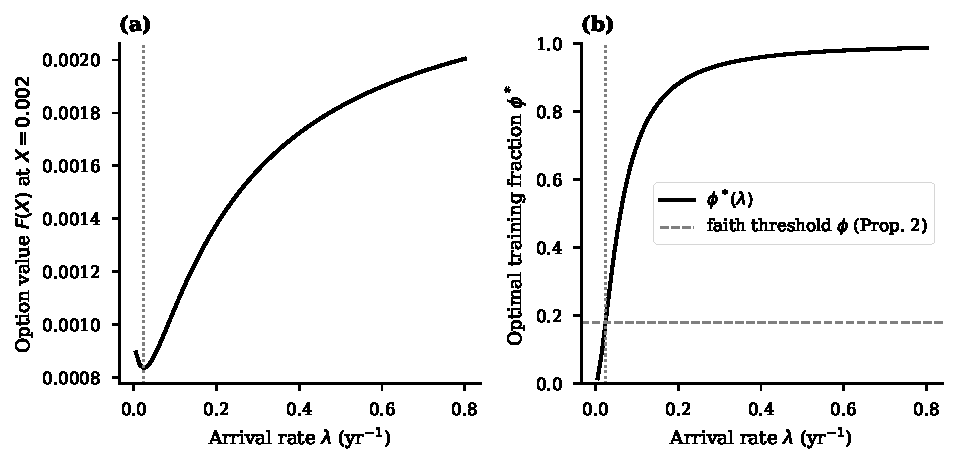
\includegraphics[keepaspectratio]{figures/fig_lambda_option_value.pdf}}

}

\caption{\label{fig-lambda-option-value}Pre-investment option value and
training allocation as a function of the arrival rate \(\lambda\) in the
full model. (a) Option value \(F(X)\) at \(X = 0.002\), with
\((X^*, K^*, \phi^*)\) re-optimized at each \(\lambda\). (b) Optimal
training fraction \(\phi^*(\lambda)\) (solid) and the faith-based
survival threshold \(\underline{\phi}\) of \textbf{?@eq-phi-underbar}
(dashed). The dotted vertical line in both panels marks the arrival rate
at which \(\phi^*\) crosses \(\underline{\phi}\), the minimum of the
value in \(\lambda\). Both panels sweep \(\lambda\) over an 80-point
grid on \([0.005, 0.80]\), holding all other parameters at the baseline
calibration; \(X = 0.002\) lies below every trigger on the grid.}

\end{figure}%

\subsection{Solution conventions and
approximations}\label{sec-conventions}

The closed forms of Section~\ref{sec-single-firm} and of the duopoly
below rest on four solution conventions. Table~\ref{tbl-domains}
collects them with the model's operating assumptions and with the
approximations whose size I have measured, so that a reader can see
which objects are exact, over what domain each result is stated, and how
large each departure is. The conventions are stated below; their
magnitudes are in the table.

\begin{longtable}[]{@{}
  >{\raggedright\arraybackslash}p{(\linewidth - 4\tabcolsep) * \real{0.1707}}
  >{\raggedright\arraybackslash}p{(\linewidth - 4\tabcolsep) * \real{0.1463}}
  >{\raggedright\arraybackslash}p{(\linewidth - 4\tabcolsep) * \real{0.6829}}@{}}
\caption{Operating assumptions, result domains, and measured
approximation sizes at the baseline calibration. Internet Appendix B
reports the underlying experiments.}\label{tbl-domains}\tabularnewline
\toprule\noalign{}
\begin{minipage}[b]{\linewidth}\raggedright
Group
\end{minipage} & \begin{minipage}[b]{\linewidth}\raggedright
Item
\end{minipage} & \begin{minipage}[b]{\linewidth}\raggedright
Statement or measured size
\end{minipage} \\
\midrule\noalign{}
\endfirsthead
\toprule\noalign{}
\begin{minipage}[b]{\linewidth}\raggedright
Group
\end{minipage} & \begin{minipage}[b]{\linewidth}\raggedright
Item
\end{minipage} & \begin{minipage}[b]{\linewidth}\raggedright
Statement or measured size
\end{minipage} \\
\midrule\noalign{}
\endhead
\bottomrule\noalign{}
\endlastfoot
Assumption & Regime-exclusive revenue & Training earns no L-regime
revenue; post-switch revenue needs no inference capacity \\
Assumption & Training as a flow & A flow proxy for capability, with no
accumulated stock \\
Assumption & Single lump & One irreversible installation, with \(\phi\)
fixed at installation \\
Domain & Proposition 1 & Requires \(\delta > 0\) and (A2) \\
Domain & Proposition 2(ii) & Fixed policy; closed form under symmetric
shares \\
Domain & Proposition 2(iii) & Common allocation, or monopoly \\
Domain & Proposition 3(i) & Existence conditional on a computed endpoint
sign; uniqueness analytical at \(\ell = 0\), computational otherwise \\
Domain & Leader's scale & Held at the monopoly-phase optimum \\
Domain & Leader's boundary & Pre-entry claim, \(\beta_H\) dilution
convention \\
Approximation & Pure power (\(A_1 = 0\)) & Value loss 2.6\% within the
precommitted-scale class, 6.9\% against the unrestricted optimum; no
pre-switch trigger in the unrestricted problem \\
Approximation & Single-boundary default & Overstates \(X_D\) by about
3\%, against faith-based survival \\
Approximation & Omitted follower default option & At most 1.5\% of the
default claim; zero at \(\ell = 0\) \\
Approximation & Par debt at \(r_c < r\) & Subsidy about 23\% of \(I\) at
\(\ell = 0.40\) \\
Approximation & \(\beta_H\) dilution & Leader's boundary \(+7\%\) versus
monopoly; \(X_P\) moves less than 1\% \\
\end{longtable}

\textbf{Unconditional-\(A_{\text{eff}}\) discounting.} All option-like
L-regime payoffs are valued with the H-regime exponent \(\beta_H\) and
the unconditional coefficient \(A_{\text{eff}}\)
(Equation~\ref{eq-a-eff}) rather than with regime-contingent value
functions: the pre-investment option takes the pure power form of
Section~\ref{sec-single-firm}, the exercise payoff is
Equation~\ref{eq-installed-value-L} whatever regime prevails at
exercise, the follower's option value is proportional to
\(X^{\beta_H}\), and the leader's monopoly-phase value discounts
follower entry by \((X/X_F^*)^{\beta_H}\). The convention delivers
Equation~\ref{eq-trigger-phi} and Equation~\ref{eq-default-boundary} and
governs every trigger in the paper. It restricts what the model prices
rather than approximating it with a small signed error: the exact object
is a piecewise free-boundary problem in which a switch above the
H-regime trigger is followed by immediate exercise. Internet Appendix B
solves that problem in a precommitted-scale version, in which the
post-switch scale is fixed at \(K_H^*\) and a closed form exists, and in
an unrestricted version, in which the firm chooses scale on arrival, so
the post-switch payoff is the exercise envelope over \(K\) and no finite
pre-switch trigger exists at baseline. Triggers and capacities are
therefore objects of the model these conventions define, while
\(\phi^*\) carries over exactly, because it maximizes \(A_{\text{eff}}\)
at every scale.

\textbf{Leader's scale in the duopoly.} The leader's capacity and
training fraction solve the \emph{monopoly-phase} problem, so
\((K_L, \phi_L)\) coincides with the single-firm optimum of Proposition
1. This does not affect the rent-equalization \emph{logic} that pins
down \(X_P\), but it does affect the level: re-optimizing for entry at
the preemption point implies a much smaller leader and a preemption
discount of \(86\%\) rather than \(43\%\) (Internet Appendix B). The
convention is conservative for the qualitative claim, while the reported
discount should not be read as an estimate of the effect's size.

\textbf{Single-boundary default.} The default boundary
Equation~\ref{eq-default-boundary} replaces the H-regime equity value by
its perpetuity component, collapsing the coupled pair \((X_D^L, X_D^H)\)
into one boundary. Unlike the first convention, this is an approximation
whose bias is signed and quantified in Table~\ref{tbl-domains}: it
overstates \(X_D\) and so errs against faith-based survival. A smaller
approximation omits the default-option term from the follower's entry
payoff.

\textbf{Par debt issuance at an exogenous coupon.} Leverage \(\ell\) and
the coupon rate \(r_c\) are exogenous, and debt is issued at par: the
firm receives \(\ell I(K)\) against a perpetual coupon
\(r_c \ell I(K)\). Because \(r_c < r\), the convention embeds an
implicit financing subsidy of \(\ell(1 - r_c/r) I(K)\)
(Table~\ref{tbl-domains}). It is a stress-test device that varies the
debt burden without solving a capital-structure problem, and it is why
the leverage comparative statics are not endogenous capital-structure
results. Fairly priced debt would require \(r_c \geq r\) at the entry
trigger.

Propositions 1--3 are exact statements about the model these conventions
define.

\subsection{Duopoly with Default Risk}\label{sec-duopoly}

I now introduce strategic interaction and leverage. Two symmetric firms
each hold options to invest in capacity and choose their
training-inference allocation.

Because the contest shares below depend on own capacity, the
separability behind the closed-form \(K^*\) fails in the duopoly: the
follower's \((K_F, \phi_F)\) are obtained numerically, while the
leader's are held at the monopoly-phase optimum
(Section~\ref{sec-conventions}), during which \(s_L = 1\).

\subsubsection{Regime-specific
competition}\label{regime-specific-competition}

Revenue in each regime is governed by a Tullock contest success function
\citep{tullock1980efficient, skaperdas1996contest} over the
regime-relevant capacity measure, so revenue depends on \emph{relative}
capacity. In the L-regime, firms compete over \emph{inference capacity}:
\begin{equation}\protect\phantomsection\label{eq-contest-L}{
\pi_i^L(X, \mathbf{K}, \boldsymbol{\phi}) = X \cdot \frac{[(1-\phi_i)K_i]^{2\alpha}}{[(1-\phi_i)K_i]^\alpha + [(1-\phi_j)K_j]^\alpha},
}\end{equation} which I write equivalently as
\(\pi_i^L = X \cdot [(1-\phi_i)K_i]^\alpha \cdot s_i^L\), where
\(s_i^L = [(1-\phi_i)K_i]^\alpha / \{[(1-\phi_i)K_i]^\alpha + [(1-\phi_j)K_j]^\alpha\}\)
is the L-regime contest share. In the H-regime, firms compete over
\emph{training compute}:
\begin{equation}\protect\phantomsection\label{eq-contest-H}{
\pi_i^H(X, \mathbf{K}, \boldsymbol{\phi}) = X \cdot \frac{(\phi_i K_i)^{2\alpha}}{(\phi_i K_i)^\alpha + (\phi_j K_j)^\alpha},
}\end{equation} with H-regime contest share
\(s_i^H = (\phi_i K_i)^\alpha / \{(\phi_i K_i)^\alpha + (\phi_j K_j)^\alpha\}\).

The specification formalizes the arms-race logic executives describe:
today what matters is the capacity to \emph{serve} demand, in a post-AGI
world the capability of a firm's \emph{models}. When \(K_j = 0\) both
shares equal one and revenue collapses to the single-firm case; under
symmetric capacities each share is \(1/2\). Under asymmetry two objects
must be kept apart: the contest share \(s_i = z^\alpha/(1+z^\alpha)\),
with \(z\) the ratio of own to rival regime-relevant capacity, is
increasing and concave in own capacity for \(\alpha < 1\), while the
revenue share \(z^{2\alpha}/(1+z^{2\alpha})\) exceeds it but, for
\(\alpha < 1/2\), still stays below the physical capacity fraction. The
specification rewards scale less than proportionally rather than
producing a winner-take-all pattern, and what asymmetry adds is revenue
expansion (Internet Appendix E bounds its contribution with the
arithmetic-mean industry-revenue benchmark).

Revenue expansion means that the leader's gain from capacity dominance
partly reflects pie expansion, not just share theft, which could amplify
preemption incentives. Internet Appendix E re-solves the equilibrium
under an arithmetic-mean industry-revenue benchmark, under which the
training fraction and the survival threshold are unchanged and only the
preemption discount moves, and discusses why the mechanisms carry over
to Cournot competition.

The training fraction enters both contests and moves a firm's position
in opposite directions across regimes: a higher \(\phi_i\) raises the
firm's H-regime share and lowers its L-regime share. Proposition 3(ii)
shows that this apparent trade-off leaves the optimal allocation
unchanged.

\subsubsection{Installed value in the
duopoly}\label{installed-value-in-the-duopoly}

The installed value for firm \(i\) in the L-regime combines inference
revenue and the expected H-regime continuation:
\begin{equation}\protect\phantomsection\label{eq-duopoly-value-L}{
V_i^L(X) = A_{\text{eff},i} \cdot X - \frac{\delta K_i}{r},
}\end{equation} where the effective revenue coefficient for firm \(i\)
is: \begin{equation}\protect\phantomsection\label{eq-a-eff-duopoly}{
A_{\text{eff},i} = \frac{[(1-\phi_i)K_i]^\alpha \cdot s_i^L}{r - \mu_L + \lambda} + \frac{\lambda}{r - \mu_L + \lambda} \cdot \frac{(\phi_i K_i)^\alpha \cdot s_i^H}{r - \mu_H}.
}\end{equation}

The H-regime value is
\(V_i^H(X) = A_H X (\phi_i K_i)^\alpha s_i^H - \delta K_i/r\). The two
terms of Equation~\ref{eq-a-eff-duopoly} carry the central trade-off,
inference revenue now against expected training revenue later, each
scaled by the corresponding contest share.

\subsubsection{Capital structure}\label{capital-structure}

Capital structure is parameterized by the leverage ratio
\(\ell = P / I(K)\), with \(P\) the face value of debt, exogenous and
common to both firms; debt is issued at par and pays a continuous coupon
\(C_D = r_c \cdot \ell \cdot I(K)\). Leverage is a \emph{stress-test
parameter}, not an equilibrium financing choice, and par issuance embeds
an implicit financing subsidy (Table~\ref{tbl-domains}), so no leverage
result below is an endogenous capital-structure result.

\subsubsection{Default boundary}\label{default-boundary}

Following \citet{leland1994corporate} and \citet{leland1996optimal},
equity holders default endogenously when equity value reaches zero, and
the optimal default boundary follows from smooth pasting. For a levered
firm with \((K_i, \phi_i)\) facing a rival with \((K_j, \phi_j)\):
\begin{equation}\protect\phantomsection\label{eq-default-boundary}{
X_D = \frac{\beta_L^-}{\beta_L^- - 1} \cdot \frac{C_D / r + \delta K_i / r}{A_{\text{eff},i}},
}\end{equation} where \(\beta_L^-\) is the negative root of the L-regime
characteristic equation, which incorporates the regime switch through
the effective discount rate \(r + \lambda\), and
\(\beta_L^-/(\beta_L^- - 1) \in (0,1)\) is the option value of waiting
before defaulting.\footnote{Replacing the H-regime equity value by its
  perpetuity component yields Equation~\ref{eq-default-boundary}
  exactly; Table~\ref{tbl-domains} reports the size and sign of the
  bias.}

\(A_{\text{eff},i}\) includes the H-regime continuation value through
the \(\lambda\) term. This is the \emph{training-survival channel}, the
route by which allocation feeds back into solvency. Because
\(A_{\text{eff},i}\) is single-peaked in \(\phi_i\) and the boundary is
inversely proportional to it, \(X_D\) is U-shaped in the training
fraction, falling up to \(\phi^*\) and rising beyond it. I call the
default-boundary implication of optimism \emph{faith-based survival}: a
higher \(\lambda\) raises the weight on the H-regime continuation value
and, when the firm trains enough for that term to matter, lowers the
boundary.

The mechanism differs from models in which the growth option is
exogenous, where a larger option unambiguously lowers the default
boundary: here the growth option is controlled by \(\phi\), and raising
\(\phi\) also cuts current inference revenue. The thresholds below are
thresholds on the effect of \emph{beliefs} at a given \(\phi_i\), not on
the effect of \(\phi_i\) itself, which at a given belief is the U-shape
just described.\footnote{The \(A_{\text{eff}}\)-channel threshold
  \(\underline{\phi}\) is independent of \(\lambda\); the exact net
  threshold \(\tilde{\phi}\), which absorbs the markup channel operating
  through the discount root, depends on it.}

\textbf{Proposition 2} (Endogenous default with faith-based survival;
levered duopoly). \emph{For a levered firm in the duopoly with fixed
capacity \((K_i, \phi_i)\) and rival \((K_j, \phi_j)\), the default
boundary \(X_D\) has the following properties:}

\emph{(i) \(X_D\) is increasing in leverage \(\ell\) and the coupon rate
\(r_c\).}

\emph{(ii) \(X_D\) is decreasing in \(\lambda\) precisely when the
training allocation is sufficiently high, and the characterization is
fully closed-form in the symmetric-shares case (\(s_i^L = s_i^H\), as
under symmetric capacities }and* allocations, or monopoly). Two channels
operate. The \(A_{\text{eff}}\) channel (higher \(\lambda\) raises the
weight on the H-regime continuation value, lowering \(X_D\)) is positive
if and only if \(\phi_i\) exceeds\emph{ \[
\underline{\phi} = \frac{\Omega}{1 + \Omega}, \quad \Omega \equiv \left(\frac{r - \mu_H}{r - \mu_L}\right)^{1/\alpha}.
\] \{\#eq-phi-underbar\} }An opposing markup channel operates through
the discount root: higher \(\lambda\) raises the effective discount rate
and pushes \(\beta_L^-/(\beta_L^- - 1)\) toward one, raising \(X_D\).
Because the \(A_{\text{eff}}\)-channel semi-elasticity is linear in the
L-regime flow and H-regime continuation terms, the net condition
\(\partial X_D / \partial \lambda < 0\) also solves in closed form: it
holds if and only if \(\phi_i\) exceeds the exact threshold\emph{ \[
\tilde{\phi} = \frac{\tilde{\Omega}}{1 + \tilde{\Omega}}, \quad \tilde{\Omega} \equiv \left[\frac{(r - \mu_H)\,(1 + m\Delta)}{(r - \mu_L) - m\lambda\Delta}\right]^{1/\alpha},
\] \{\#eq-phi-tilde\} }where \(\Delta = r - \mu_L + \lambda\) and
\(m = \mathrm{d}\ln M / \mathrm{d}\lambda = 1/[\beta_L^-(\beta_L^- - 1)\mathcal{R}] > 0\)
is the markup-channel semi-elasticity, with
\(\mathcal{R} = \sqrt{(\mu_L - \sigma^2/2)^2 + 2\sigma^2(r+\lambda)}\)
(Internet Appendix A states the mild regularity condition). The exact
threshold nests \(\underline{\phi}\) as the \(m \to 0\) limit and
satisfies \(\tilde{\phi} > \underline{\phi}\). Unlike
\(\underline{\phi}\), \(\tilde{\phi}\) depends on \(\lambda\). Finally,
\(\underline{\phi}\) is increasing in \(\alpha\) (with less concavity in
the revenue function, a larger training allocation is needed for the
H-regime term to dominate), decreasing in \(\mu_H - \mu_L\) (a larger
regime-switch growth premium amplifies the H-regime term, lowering the
threshold), and increasing in \(r\) (higher discounting reduces the
present value of the continuation opportunity).*

\emph{(iii) For a given capacity \(K\) and training fraction \(\phi_i\)
below the interior maximizer of \(A_{\text{eff},i}(\cdot)\), there
exists a leverage-training substitution along the iso-\(X_D\) locus: a
firm can maintain the same default boundary \(X_D\) while increasing
leverage (which raises the coupon obligation in the numerator) by
simultaneously increasing the training fraction (which raises
\(A_{\text{eff},i}\) through the H-regime term in the denominator). This
is a mechanical relationship describing the set of \((\ell, \phi)\)
pairs consistent with a given default boundary, not a statement about
optimality: in the solved model the optimal training fraction is
invariant to leverage, since the allocation first-order condition does
not involve \(\ell\).}

\emph{(iv) \(X_D\) is increasing in rival capacity \(K_j\), because
higher rival capacity reduces the contest shares \(s_i^L\) and
\(s_i^H\).}

Parts (i)--(iv) hold at fixed \((K, \phi, \ell)\), a domain
Table~\ref{tbl-domains} records; part (i) is a stress-test comparative
static rather than a statement about an optimally chosen capital
structure, as are Proposition 3(iv) and Section~\ref{sec-valuation}.
Under joint re-optimization, higher \(\lambda\) also raises \(\phi^*\)
(Proposition 1), but because \(\phi^*\) maximizes \(A_{\text{eff}}\),
this induced reallocation has no first-order effect on \(X_D\) (an
envelope argument; at baseline about \(4\%\) of the direct effect of
moving \(\lambda\) from \(0.10\) to \(0.11\)). Three experiments should
be kept apart. Raising \(\lambda\) at a fixed policy lowers \(X_D\) if
and only if \(\phi_i > \tilde{\phi}\) (part ii). Raising \(\phi_i\) at a
fixed belief lowers \(X_D\) if and only if \(\phi_i < \phi^*\), and
raises it beyond. Comparing firms that re-optimize under different
beliefs combines the two: along the locus of optimal policies
\(X_D(\phi^*(\lambda), \lambda)\) is decreasing in \(\lambda\) for
\(\lambda \gtrsim 0.034\) at baseline, so a more optimistic firm trains
more \emph{and} sits further from default, but it is the belief, not the
training fraction, that does the work. Because the optimal training
fraction is invariant to leverage, part (iii) carries an empirical
caveat: observed comovement between leverage and training allocation
would reflect joint determination rather than a causal link.

At baseline, \(\Omega \approx 0.22\), \(\underline{\phi} \approx 0.18\),
and \(\tilde{\phi} \approx 0.32\) against \(\phi^* \approx 0.70\), so
faith-based survival holds at the optimum. Because \(\tilde{\phi}\)
depends on \(\lambda\), the ranking reverses for
\(\lambda \lesssim 0.034\), where the optimal allocation is too
inference-heavy for the training-survival channel to dominate.

Figure~\ref{fig-default-boundaries} shows how leverage moves the
triggers and the default boundary in the equilibrium characterized
below, in which the \emph{leader} invests first at \(X_P\) and the
\emph{follower} later at \(X_F^*\). As leverage rises the follower
invests later and at larger scale, because the below-market coupon
lowers the effective capital cost: \(X_F^*\) rises from about \(0.12\)
at \(\ell = 0.05\) to \(0.21\) at \(\ell = 0.65\), while
\(X_F^*/X_{D,F}\) falls from about \(12\) to \(6\). That compressed
distance to default is the scenario Amodei describes, in which a firm
committed to trillion-dollar compute purchases faces bankruptcy if
revenue falls modestly short \citep{amodei2026dwarkesh}.

\begin{figure}[!htb]

\centering{

\pandocbounded{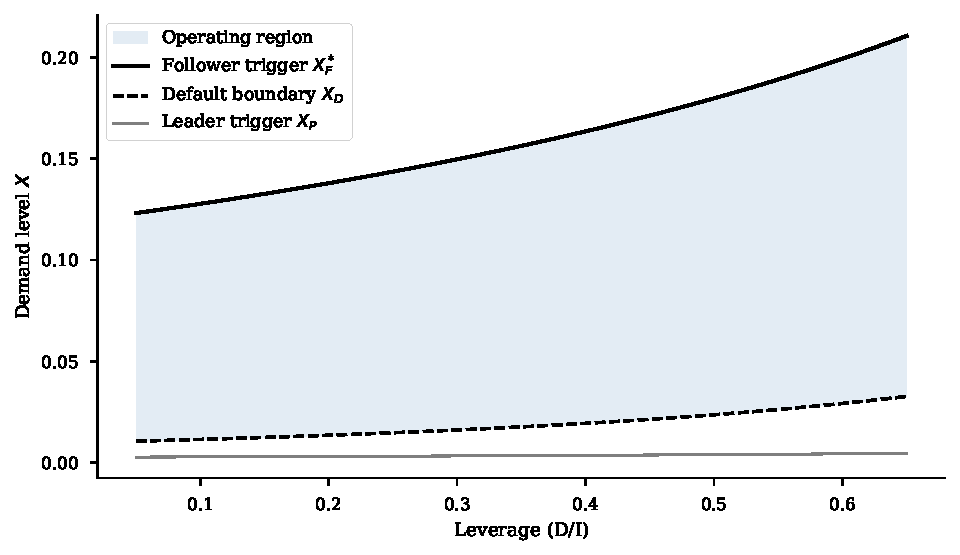
\includegraphics[keepaspectratio]{figures/fig_default_boundaries.pdf}}

}

\caption{\label{fig-default-boundaries}Investment and default boundaries
as a function of leverage in the duopoly equilibrium. The solid line
shows the follower's trigger \(X_F^*\); the dashed line shows the
follower's default boundary \(X_{D,F}\); the gray solid line shows the
leader's preemption trigger \(X_P\) and the gray dash-dotted line the
leader's default boundary \(X_{D,L}\) (the anticipating leader's
boundary of Internet Appendix A). The shaded band between \(X_{D,F}\)
and \(X_F^*\) is the follower's post-entry continuation band: an
installed follower also operates above \(X_F^*\), and a follower that
has not yet entered is waiting below it. The vertical axis is
logarithmic, so equal vertical distances correspond to equal
proportional distances to the default boundary. The equilibrium is
re-solved at each of 40 leverage levels spanning
\(\ell \in [0.05, 0.65]\): the follower's capacity and training fraction
are re-optimized at every level, while the leader's are held at the
monopoly-phase optimum under the leader-scale convention of
Section~\ref{sec-conventions}. Parameters: baseline calibration with
coupon rate \(r_c = 0.05\) and bankruptcy cost \(b = 0.30\).}

\end{figure}%

\subsubsection{Equity and debt values}\label{equity-and-debt-values}

Following \citet{leland1994corporate}, \(E(X)\) is the
\emph{going-concern} equity value once investment is sunk, and the
object relevant for timing is the entry NPV \(E(X) - (1-\ell)I(K)\).
This is the single equity convention used in the paper, the proofs, and
the code: limited liability floors \(E\), not the entry NPV. The equity
contribution is sunk and is not refunded on default, so the entry NPV is
strictly negative at low demand, the boundary condition on which
Proposition 3(i) rests. Above the default boundary:
\begin{equation}\protect\phantomsection\label{eq-equity}{
E(X) = A_{\text{eff},i}\, X - \frac{\delta K}{r} - \frac{C_D}{r} + \left[\frac{C_D}{r} + \frac{\delta K}{r} - A_{\text{eff},i}\, X_D \right]\left(\frac{X}{X_D}\right)^{\beta_L^-},
}\end{equation} where \(\beta_L^- < 0\). The last term is the default
option and the bracket the flow deficit at the boundary; value-matching
and smooth-pasting on \(E\) pin down \(X_D\) in
Equation~\ref{eq-default-boundary}. At \(X = X_D\), \(E(X_D) = 0\) and
the entry NPV equals \(-(1-\ell)I(K) < 0\), as below \(X_D\). Without
debt, \(E(X)\) is the unlevered perpetuity, with no abandonment
option.\footnote{Omitting that option is conservative and negligible,
  because the firm invests at \(X^*\) well above any abandonment
  threshold.}

Debt value is: \[
D(X) = \frac{C_D}{r}\left[1 - \left(\frac{X}{X_D}\right)^{\beta_L^-}\right] + R(X_D) \left(\frac{X}{X_D}\right)^{\beta_L^-},
\] where the recovery in default is \[
R(X_D) = \min\left\{(1 - b)\,\Lambda(X_D),\; \frac{C_D}{r}\right\}, \quad \Lambda(X_D) = \frac{[(1-\phi_i)K_i]^\alpha \, s_i^L}{r - \mu_L + \lambda}\, X_D,
\] \(b \in [0,1]\) is the fraction of liquidation value lost in
bankruptcy and \(\Lambda(X_D)\) the liquidation value of productive
assets. Only the \emph{inference} business survives liquidation, while
the H-regime continuation value is destroyed, because the post-AGI
payoff requires the going concern. The asymmetry is central to
Section~\ref{sec-valuation}: faith-based survival lowers the
\emph{probability} of default, but faith is worthless to creditors
\emph{in} default, so training raises the loss given default.

\subsubsection{Preemption equilibrium}\label{preemption-equilibrium}

I solve the timing game by backward induction under the conventions of
Section~\ref{sec-conventions}; the object characterized is the
equilibrium of the model those conventions define, a tractable benchmark
rather than the subgame-perfect equilibrium of the unrestricted game. It
has no closed form: the follower's \((K_F, \phi_F)\) solve a fixed point
in which the entry trigger is recomputed by smooth pasting at each
evaluation, and \(X_P\) follows by root-finding on \(L(X) - F(X)\).
Investment is publicly observed. I follow the preemption construction of
\citet{fudenberg1985preemption}, extended to asymmetric capacity choice
by \citet{huisman2015strategic} and \citet{pawlina2006real}, whose two
underwriting conditions are verified computationally at every
parameterization tested.

\textbf{Follower's problem.} The follower observes \((K_L, \phi_L)\) and
chooses \(X_F^*\), \(K_F\), and \(\phi_F\) to maximize its option value.
Leverage cannot be a free choice variable: the implicit financing
subsidy makes the objective strictly increasing in \(\ell\), so an
unconstrained choice would be the degenerate corner \(\ell = 1\).

\textbf{Leader's problem.} The leader accounts for the follower's entry,
which dilutes its contest share in both regimes: before entry it earns
monopoly revenue with \(s_L = 1\), afterwards revenue is shared. With
debt, the leader's default boundary is solved on the pre-entry claim
including the anticipated dilution, so it lies above the monopoly
boundary of Equation~\ref{eq-default-boundary} (Internet Appendix A,
Table~\ref{tbl-domains}).

\textbf{Preemption trigger.} Both firms share the same \(\lambda\) and
the equilibrium is symmetric; cross-sectional variation in investment
behavior (Section~\ref{sec-calibration}, Section~\ref{sec-valuation})
comes from comparative statics across archetypes, not from interaction
among firms with different priors. Both would like to lead, and \(X_P\)
solves \(L(X_P) = F(X_P)\), with \(L(X) = E_L(X) - (1-\ell)I(K_L)\) the
leader's entry NPV. At \(X_P\) the rent from leading is fully
dissipated.

\textbf{Default, entry, and what the equilibrium does not cover.}
Default is the endogenous stopping decision of
Equation~\ref{eq-default-boundary}: equity holders abandon the firm at
\(X_D\), creditors recover \(R(X_D)\), and only the inference business
is realized in liquidation. Entry is the exercise of an investment
option: the leader installs \((K_L, \phi_L)\) at \(X_P\) and the
follower \((K_F, \phi_F)\) at \(X_F^*\), after which
Equation~\ref{eq-contest-L} and Equation~\ref{eq-contest-H} govern both
firms' revenue. What happens once a firm defaults lies outside the
equilibrium characterized here: the recovery formula values the
liquidated inference assets but does not say who operates them, so it
determines neither the survivor's revenue nor the opportunity of a
follower that has not yet entered when the leader defaults. The
fixed-rival formulas Equation~\ref{eq-a-eff-duopoly},
Equation~\ref{eq-default-boundary}, and Equation~\ref{eq-equity} hold
\((K_j, \phi_j)\) fixed and cover neither subgame; all quantities below
are computed on the path along which both firms remain solvent.

\textbf{Proposition 3} (Preemption equilibrium with training allocation
and default risk; symmetric duopoly). \emph{In the symmetric duopoly
with leverage \(\ell\), under the solution conventions of
Section~\ref{sec-conventions}:}

\emph{(i) (Existence: conditional analytical, by the intermediate value
theorem with the upper endpoint sign verified computationally;
Uniqueness: analytical for \(\ell = 0\), computational for \(\ell > 0\))
A preemption trigger \(X_P \in (0, X_L^{\text{mono}})\) exists such that
\(L(X_P) = F(X_P)\), where \(L(X) = E_L(X) - (1-\ell)I(K_L)\) is the
leader's NPV of entering at state \(X\) with \(E_L\) the going-concern
equity value, \(F(X)\) is the follower's option value, and
\(X_L^{\text{mono}}\) is the leader's monopoly-only trigger, the trigger
it would choose with no rival. Existence follows from continuity and the
boundary conditions \(L(0) < F(0)\) and
\(L(X_L^{\text{mono}}) > F(X_L^{\text{mono}})\) (Internet Appendix A).
The lower-endpoint inequality is analytical, since the sunk equity
contribution makes \(L(0) < 0 = F(0)\), while the upper-endpoint
inequality is verified computationally at every parameterization tested,
so existence is analytical conditional on that sign. At zero leverage
the gap \(L(X) - F(X)\) is strictly concave on \((0, X_F^*)\) and
negative at the origin, so the up-crossing is unique analytically
(Internet Appendix A); under leverage the default-option term breaks
global concavity near \(X_D\), and uniqueness is verified
computationally across all parameterizations, with no case of multiple
up-crossings found (Internet Appendix B).}

\emph{(ii) (Analytical critical point; global optimality computational)
The training fraction is invariant to competitive role:
\(\phi_L^* = \phi_F^* = \phi^*\), the single-firm optimum of Proposition
1. The invariance follows from the factorization of the regime-specific
contest structure (Internet Appendix A), so \(\phi^*\) is an exact
critical point of the follower's allocation problem for any capacities;
that it is the global maximizer is verified computationally. Training
allocation is pinned down by beliefs and technology, not by market
position.}

\emph{(iii) (Numerical finding) Higher \(\lambda\) increases \(\phi^*\)
for both firms and lowers the preemption trigger \(X_P\).}

\emph{(iv) (Numerical finding; exogenous \((\ell, r_c)\)) Higher
leverage increases the follower's capacity \(K_F\) and raises all three
boundaries \(X_P\), \(X_F^*\), and \(X_D\): par-issued debt with a
below-market coupon lowers the effective capital cost (a modelling
convention of Section~\ref{sec-conventions}, not an equilibrium
financing outcome), supporting larger scale that requires higher demand
to justify, while the coupon obligation raises the default point. The
distance to default \(X_F^*/X_D\) falls with leverage.}

\emph{(v) (Numerical finding) The leader's distance to default at entry,
\(X_P/X_D\), is decreasing in \(\lambda\): firms with higher \(\lambda\)
invest earlier and enter closer to their default boundary, and the
credit spread at entry is correspondingly weakly increasing in
\(\lambda\).}

Role-invariance has a straightforward reading. Both contests run over
the \emph{same} installed capacity, scaled by \(\phi\) in the H-regime
and by \(1 - \phi\) in the L-regime, so a common change in \(\phi\)
moves both shares by the same factor and drops out of the ratio of
marginal values. Rivalry changes how much a firm builds and when, not
how it splits it.

Figure~\ref{fig-competition-effect} plots the monopolist's trigger
alongside the duopoly leader's preemption trigger against volatility.
Over the admissible grid \(\sigma \in [0.20, 0.30]\), which starts just
above the lower bound (A2) imposes, the leader invests strictly earlier
than the monopolist and the gap widens with \(\sigma\). The ratio
\(X_P/X_L^{\text{mono}}\) falls from about \(0.64\) to \(0.54\) and is
about \(0.57\) at baseline, a preemption discount of roughly \(43\%\).
That magnitude is conditional on the leader-scale convention:
re-optimizing the leader's scale raises it to \(86\%\)
(Section~\ref{sec-conventions}). The sign is robust to the convention;
the magnitude is not.

\begin{figure}[!htb]

\centering{

\pandocbounded{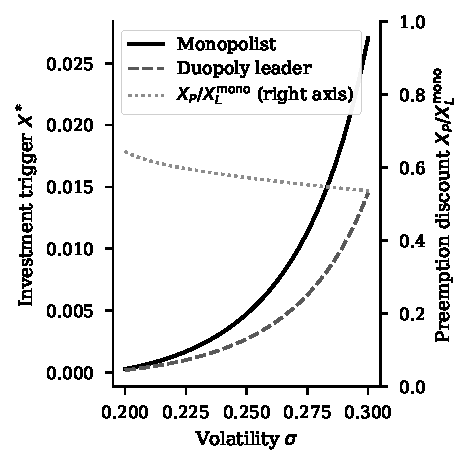
\includegraphics[keepaspectratio]{figures/fig_competition_effect.pdf}}

}

\caption{\label{fig-competition-effect}Monopolist and duopoly-leader
investment triggers as a function of volatility \(\sigma\). The solid
line is the monopolist's trigger \(X_L^{\text{mono}}\) and the dashed
line the duopoly leader's preemption trigger \(X_P\); the dotted line
(right axis) plots the trigger ratio \(X_P / X_L^{\text{mono}}\). The
equilibrium is re-solved at each of 30 points on the grid
\(\sigma \in [0.20, 0.30]\), which starts just above the admissibility
bound of condition (A2) (Internet Appendix B). Zero-leverage duopoly;
all other parameters at baseline values. The leader's capacity and
training fraction are held at the monopoly-phase optimum (the
leader-scale convention of Section~\ref{sec-conventions}), on which the
level of \(X_P\) depends: re-optimizing the leader's scale for entry at
\(X_P\) roughly doubles the preemption discount (Internet Appendix B).}

\end{figure}%

\textbf{The leader--follower scale asymmetry.} The equilibrium is
starkly asymmetric in scale as well as timing: at baseline the follower
installs \(K_F \approx 0.259\) against the leader's
\(K_L \approx 0.0067\) and enters at \(X_F^* \approx 0.119\) against
\(X_P \approx 0.0027\). The direction follows from an elasticity wedge,
the follower's marginal revenue elasticity being \(\alpha(2 - s_F)\)
rather than \(\alpha\), which the capacity first-order condition
amplifies near the (A2) boundary; the magnitude is a joint property of
the contest and of the baseline calibration, not a robust prediction
(Internet Appendix B). The ``leader'' here is therefore not the dominant
incumbent of the AI-rivalry narrative but a small, early, preemptive
commitment, while the ``follower'' waits for demand and then builds at
scale. What the model rules out is a leader that stays large, so the
paper's claims about leadership concern the \emph{timing} margin only.

Propositions 1 and 2 are fully analytical; Proposition 3 combines
conditional-analytical existence, zero-leverage uniqueness, and an exact
allocation fixed point with computational verification of the rest
(Table~\ref{tbl-result-taxonomy}).

\section{Quantitative Calibration}\label{sec-calibration}

The calibration maps the model parameters to the AI infrastructure
sector using company filings, industry reports, and the scaling laws
literature. It is \emph{stylized}: the goal is to discipline the model's
quantitative magnitudes and illustrate cross-sectional heterogeneity,
not to estimate firm-level primitives or test the model empirically. Two
caveats apply throughout. First, the Leland default framework is a
tractable approximation to financial distress risk that fits public-debt
issuers better than VC-backed labs, though the qualitative predictions
apply across financing structures (see Section~\ref{sec-discussion};
Internet Appendix C). Second, the training fractions \(\hat{\phi}\) are
assigned by judgment from incomplete evidence and carry substantial
uncertainty (\(\pm 0.10\)).

\subsection{Demand Process}\label{demand-process}

I use regime-dependent drifts \(\mu_L = 0.01\) and \(\mu_H = 0.06\),
common volatility \(\sigma = 0.25\), and an arrival rate
\(\lambda = 0.10\) per year, implying an expected 10 years to the regime
switch; all four are chosen rather than estimated. The drifts are
\emph{risk-adjusted} (certainty-equivalent) rates, not observed revenue
growth, so the 24--39\% cloud revenue growth in Table~\ref{tbl-sources}
in the Internet Appendix is consistent with a much lower \(\mu_H\). The
demand shifter \(X\) is latent, so no observable series identifies
\(\sigma\); the interior-capacity condition (A2) below admits
\(\sigma \in (0.19, 0.39)\) at baseline, and \(\sigma = 0.25\) sits
inside that window. The baseline \(\lambda\) is a moderate prior: it is
more conservative than the beliefs implied by \citet{amodei2024machines}
(\(\lambda \approx 0.30\)--\(0.50\)) and sits at the lower endpoint of
the range implied by Hassabis's public statements
(\(\lambda \approx 0.10\)--\(0.15\)). That dispersion of beliefs is what
generates the cross-sectional variation analyzed in
Section~\ref{sec-valuation}.

The baseline discount rate \(r = 0.12\) is a risk-adjusted WACC chosen
to represent a frontier AI lab rather than estimated from one firm's
data; as in Section~\ref{sec-model} ({Footnote \ref{fn:wacc}}), \(r\) is
the WACC and \(\mu_s\) is net of a risk premium. It exceeds typical
corporate WACCs because frontier AI labs carry substantial technology
risk and elevated costs of equity (Internet Appendix C). Condition (A2),
\(1/\gamma < (\beta_H - 1)/(\alpha\beta_H) < 1\), admits only
\(r \in (0.097, 0.135)\), so the Google-like (\(0.10\)) and baseline
cases lie inside the window while the OpenAI-like (\(0.14\)),
Anthropic-like (\(0.15\)), and xAI-like (\(0.18\)) archetypes violate
its upper bound. Every trigger and capacity result is therefore computed
at the baseline WACC; archetype-specific WACCs enter only through the
capacity-free inversion
\(\lambda = (\hat{\phi}/(1-\hat{\phi}))^{1-\alpha}(r - \mu_H)\) below
(Internet Appendix B).

\subsection{Technology Parameters}\label{technology-parameters}

The revenue elasticity \(\alpha = 0.40\) governs diminishing returns to
capacity, entering both the L-regime inference contest
(Equation~\ref{eq-contest-L}) and the H-regime training contest
(Equation~\ref{eq-contest-H}). The compute-to-loss power laws in
\citet{kaplan2020scaling} and \citet{hoffmann2022training} motivate a
concave revenue technology but do not measure \(\alpha\): a loss
exponent is not a revenue elasticity, so \(\alpha = 0.40\) is a chosen
value. Condition (A2) admits only \(\alpha \in (0.356, 0.534)\), placing
\(\alpha = 0.40\) near the lower bound, and the trigger and capacity are
highly sensitive to it there, with elasticities of \(+19.7\) and
\(+24.2\) (Table~\ref{tbl-elasticities} in the Internet Appendix). That
sensitivity is why the paper reports ratios and percentage differences
rather than levels. The cost function \(I(K) = cK^\gamma\) with
convexity \(\gamma = 1.50\) captures increasing marginal costs from
power constraints, supply chain bottlenecks, and site preparation, and I
normalize the unit cost \(c = 1.0\).

The operating cost rate \(\delta = 0.03\) is the flow cost of
maintaining installed capacity (power, cooling, maintenance, personnel),
distinct from depreciation of GPU hardware, whose capital cost sits in
\(cK^\gamma\). It is likewise chosen, and nothing substantive turns on
it: \(\delta\) enters only through the total cost
\(b(K) = \delta K/r + cK^\gamma\), so a change in \(\delta\) is
equivalent to a rescaling of the capacity unit and leaves \(\phi^*\),
the trigger ratio, and the Dario's dilemma losses unchanged (Internet
Appendix C). Table~\ref{tbl-parameters} in the Internet Appendix records
the calibration status of every parameter.

\subsection{Stylized Firm Archetypes}\label{stylized-firm-archetypes}

I construct four stylized firm archetypes spanning the cross-sectional
variation in leverage, discount rate, and training allocation. They are
\emph{illustrative composites}, not structural estimates of any specific
company's parameters; Internet Appendix C documents the sourcing
archetype by archetype and Table~\ref{tbl-sources} there lists the
sources. For the three archetypes modelled on privately held firms
(Anthropic-like, OpenAI-like, and xAI-like), the values rest on press
reports rather than audited filings and carry lower confidence than the
Google-like archetype's. Because the underlying revenue and
capital-expenditure concepts are not harmonized, the columns of
Table~\ref{tbl-firms} are model inputs, not measured cross-sectional
moments.

\begin{longtable}[]{@{}
  >{\raggedright\arraybackslash}p{(\linewidth - 8\tabcolsep) * \real{0.2600}}
  >{\raggedright\arraybackslash}p{(\linewidth - 8\tabcolsep) * \real{0.1800}}
  >{\raggedright\arraybackslash}p{(\linewidth - 8\tabcolsep) * \real{0.1800}}
  >{\raggedright\arraybackslash}p{(\linewidth - 8\tabcolsep) * \real{0.1800}}
  >{\raggedright\arraybackslash}p{(\linewidth - 8\tabcolsep) * \real{0.2000}}@{}}
\caption{Stylized firm archetypes: calibration inputs, as of Q4 2025--Q1
2026. \(\hat{\phi}\) is the training fraction \emph{assigned} to each
archetype by judgment from executive statements
\citep{amodei2026dwarkesh}, Epoch AI's reconstruction of OpenAI's 2024
compute, and Deloitte's TMT Predictions 2026 (Internet Appendix C); it
is not an observed quantity and is distinct from the model's endogenous
training fraction \(\phi\). The implied \(\lambda\) band inverts the
closed-form training-allocation first-order condition at
\(\hat{\phi} \pm 0.10\), holding \(r\) at the common baseline; revenue
and capital-expenditure inputs are also in Internet Appendix C. All
values are order-of-magnitude composites, not precise
calibrations.}\label{tbl-firms}\tabularnewline
\toprule\noalign{}
\begin{minipage}[b]{\linewidth}\raggedright
Calibration input
\end{minipage} & \begin{minipage}[b]{\linewidth}\raggedright
Frontier Lab
\end{minipage} & \begin{minipage}[b]{\linewidth}\raggedright
Platform
\end{minipage} & \begin{minipage}[b]{\linewidth}\raggedright
Hyperscaler
\end{minipage} & \begin{minipage}[b]{\linewidth}\raggedright
Compute Racer
\end{minipage} \\
\midrule\noalign{}
\endfirsthead
\toprule\noalign{}
\begin{minipage}[b]{\linewidth}\raggedright
Calibration input
\end{minipage} & \begin{minipage}[b]{\linewidth}\raggedright
Frontier Lab
\end{minipage} & \begin{minipage}[b]{\linewidth}\raggedright
Platform
\end{minipage} & \begin{minipage}[b]{\linewidth}\raggedright
Hyperscaler
\end{minipage} & \begin{minipage}[b]{\linewidth}\raggedright
Compute Racer
\end{minipage} \\
\midrule\noalign{}
\endhead
\bottomrule\noalign{}
\endlastfoot
Reference firm (illustrative) & Anthropic-like & OpenAI-like &
Google-like & xAI-like \\
Assigned training fraction \(\hat{\phi}\) & 0.55 & 0.60 & 0.35 & 0.75 \\
Uncertainty band on \(\hat{\phi}\) & \(\pm 0.10\) & \(\pm 0.10\) &
\(\pm 0.10\) & \(\pm 0.10\) \\
Implied \(\lambda\) band at \(r = 0.12\) & {[}0.05, 0.09{]} & {[}0.06,
0.10{]} & {[}0.03, 0.05{]} & {[}0.09, 0.17{]} \\
Leverage (debt / total capital) & 0.05 & 0.05 & 0.10 & 0.15 \\
WACC (per year) & 0.15 & 0.14 & 0.10 & 0.18 \\
\end{longtable}

The training fraction \(\hat{\phi}\) is my assigned share of compute
allocated to training rather than to inference serving, triangulated
from executive statements, Epoch AI's reconstruction of OpenAI's 2024
spend, and industry-wide trajectory estimates (Internet Appendix C).
Firms do not disclose precise training-inference breakdowns, so each
entry carries uncertainty of roughly \(\pm 0.10\). Because \(\phi^*\)
varies slowly with \(\lambda\)
(\(\varepsilon_{\phi^*,\lambda} = (1-\phi^*)/(1-\alpha) \approx +0.5\)
at baseline), the inverse mapping is steep: inverting the allocation
first-order condition at \(\hat{\phi} \pm 0.10\) yields implied arrival
rates spanning roughly a factor of two, with the xAI-like archetype
implying \(\lambda \in [0.09, 0.17]\) (6--11 years) and the Google-like
hyperscaler \(\lambda \in [0.03, 0.05]\) (19--32 years). Because the
\(\hat{\phi}\) values are assigned rather than measured, the inversion
is a scenario map from allocations to the beliefs that would rationalize
them; it is not evidence that beliefs explain observed differences
across firms.

Leverage is low by construction: the Anthropic-like and OpenAI-like
archetypes are effectively all-equity funded (\(\ell = 0.05\)), the
xAI-like archetype carries \(\ell = 0.15\) on its secured debt, and even
the hyperscaler carries only modest debt (\(\ell = 0.10\)). These are
round assumptions rather than measured market-value debt-to-capital
ratios (Internet Appendix C), meant to capture the venture-backed
financing of AI labs.

\subsection{Baseline Results}\label{baseline-results}

Under the baseline calibration, the single-firm model produces an
investment trigger \(X^* \approx 0.0047\), capacity
\(K^* \approx 0.0067\), and training fraction \(\phi^* \approx 0.70\),
where the effective revenue coefficient \(A_{\text{eff}}\)
(Equation~\ref{eq-a-eff}) combines L-regime inference value and H-regime
training value. By the solution convention discussed after Proposition
1, the duopoly leader's monopoly policy coincides with this optimum, so
\(X_L^{\text{mono}} = X^* \approx 0.0047\); the zero-leverage duopoly
equilibrium produces a follower policy of \(X_F^* \approx 0.12\),
\(K_F \approx 0.26\), and \(\phi_F^* \approx 0.70\), with the leader
preempting at \(X_P \approx 0.0027\) (Section~\ref{sec-duopoly}).
Because \(c = 1\) fixes the cost scale by normalization, the levels of
\(K\) and \(X\) are not physical units and the quantitative content
resides in \emph{ratios} and \emph{percentages}: the trigger ratio
\(X_P / X_L^{\text{mono}} \approx 0.57\) (conditional on the
leader-scale convention; Internet Appendix B), \(\phi^* \approx 0.70\),
the value-loss asymmetry (26\% versus 6\%), and the leverage gradient of
credit spreads (Section~\ref{sec-valuation}). Mapping to observable
units means setting \(c\) so that \(I(K) = cK^\gamma\) matches observed
CapEx: at \(c \approx \$23\text{B}\) the follower's investment cost
\(I(K_F) = K_F^{1.5} \approx 0.13\) maps to approximately \$3B, the
Anthropic-like archetype's annual CapEx. That rescaling is a change of
units: with \(\kappa = c^{1/(\gamma-1)}\), the optimal policy transforms
as \(K \to K/\kappa\) and \(X \to X/\kappa^{1-\alpha}\) and values scale
by \(\kappa\), so every ratio and percentage reported in the paper is
unchanged, while the credit spreads and default probabilities of
Section~\ref{sec-valuation} and Internet Appendix H, evaluated at a
fixed \((X, K)\), are invariant only if that evaluation point is
rescaled with the units.

\subsection{Sensitivity Analysis}\label{sensitivity-analysis}

Table~\ref{tbl-elasticities} in the Internet Appendix reports
elasticities of the optimal policy at the baseline; Internet Appendix D
develops the comparative statics and Internet Appendix E the
\(\pm 25\%\) parameter-perturbation sweep. The signs are the standard
real-options ones: within the model, a higher \(\lambda\) lowers the
trigger and raises \(\phi^*\), so more optimistic firms invest earlier
and train more. The elasticities with respect to \(r\) and \(\alpha\)
are large, so these comparative statics are read as directions rather
than magnitudes, inside the admissible (A2) window.

\section{Quantitative Implications}\label{sec-valuation}

Three quantitative implications follow from the model: a scale-gap
diagnostic, endogenous credit risk, and Dario's dilemma, the asymmetric
cost of investing on a mistaken belief about \(\lambda\). All results
here are numerical, computed under the stylized calibration of
Section~\ref{sec-calibration}, and illustrate the model's mechanisms
rather than delivering point estimates. Motivated by
\citet{berk1999optimal}, Internet Appendix G develops a unit-free
\emph{scale-gap index} measuring the distance between a firm's installed
base and the model's optimal scale; because the model does not identify
levels, its content is the shape of the curve rather than any firm's
position along it (Figure~\ref{fig-growth-decomposition}).

\subsection{Credit Risk Analysis}\label{credit-risk-analysis}

Leverage, training allocation, demand uncertainty, and competition
jointly generate credit risk; Internet Appendix H gives the spread and
default-probability formulas, their measure qualifications, and the
leverage curves (Figure~\ref{fig-credit-risk}). The training fraction
\(\phi\) enters through two opposing channels. Below the allocation
optimum, a higher \(\phi\) raises \(A_{\text{eff}}\) and lowers the
default boundary \(X_D\) (the training-survival channel of Proposition
2; the sign reverses above \(\phi^*\)), reducing the \emph{probability}
of default. The recovery specification (Section~\ref{sec-duopoly}) works
against this: a higher \(\phi\) shrinks the inference business creditors
can liquidate, raising the \emph{loss given default}. At baseline the
second channel modestly dominates, so spreads are mildly increasing in
\(\phi\) at a given leverage even as default probabilities fall; that
decomposition is what testable prediction 1 in
Section~\ref{sec-discussion} proposes to test. At a fixed \(X = 0.10\)
with \(K = 1\) and \(\phi = 0.5\), the spread is zero at \(\ell = 0.05\)
and rises to 12, 41, and 97 bps at \(\ell = 0.20\), \(0.40\), and
\(0.70\), while the five-year default probability rises from 0.63\% to
1.80\%, 4.85\%, and 12.98\%. Both are \emph{model-implied risk-adjusted}
objects rather than risk-neutral quantities, and because \(\ell\) and
\(r_c\) are exogenous stress-test parameters (Section~\ref{sec-model}),
they describe the response to an imposed debt burden rather than the
optimal policy.

\subsection{Dario's Dilemma}\label{darios-dilemma}

The probability of a regime switch within five years is
\(1 - e^{-5\lambda} = 39\%\) at the baseline \(\lambda = 0.10\) and 92\%
at \(\lambda = 0.50\), so beliefs across the range of disagreement
documented in Section~\ref{sec-calibration} imply large differences in
investment (the option value itself is not monotone in \(\lambda\) at
the lowest rates; Remark 3). I now quantify the cost of belief
mismatches, which I call \emph{Dario's dilemma}: the tension between
building aggressively for an AI future and managing the financial risk
of overinvestment.

\subsubsection{Setup}\label{setup}

Consider a firm with true private belief \(\lambda_{\text{true}}\) that
invests according to
\(\lambda_{\text{invest}} \neq \lambda_{\text{true}}\), choosing
trigger, capacity, and training fraction optimally for that possibly
incorrect belief. Agency problems, strategic signaling, and bounded
rationality could each produce such a mismatch, none of which the model
contains: it takes \(\lambda_{\text{invest}}\) as given and prices the
mismatch rather than deriving it.

\subsubsection{Value Loss}\label{value-loss}

The value loss from mismatch is \[
\Delta V = \text{NPV}(\lambda_{\text{true}}, \lambda_{\text{true}}) - \text{NPV}(\lambda_{\text{true}}, \lambda_{\text{invest}}),
\] where \(\text{NPV}(\lambda_a, \lambda_b)\) is the expected present
value, at a common initial demand level \(X_0\), of the policy
\((X^*, K^*, \phi^*)\) optimal for belief \(\lambda_b\) when the true
demand process is governed by \(\lambda_a\), with the timing discount
\((X_0/X^*)^{\beta_H}\) adjusting for different waiting times.
Percentage losses are reported as
\(\Delta V / \text{NPV}(\lambda_{\text{true}}, \lambda_{\text{true}})\).
The levered version keeps the same operating policy and changes only the
claim being valued: \(\text{NPV}\) then denotes the total claims net of
the investment outlay, \(E + D - I(K^*)\) with \(E\) the going-concern
equity of Section~\ref{sec-duopoly}. Because that policy is not
re-optimized against the levered objective, the levered value function
is maximized very nearly, but not exactly, at
\(\lambda_{\text{invest}} = \lambda_{\text{true}}\); the resulting
shortfall is three orders of magnitude below the mismatch losses
reported here (Internet Appendix A).

\textbf{Numerical Finding 1} (Dario's dilemma). \emph{Across all
parameterizations tested, the value loss from conservative
underinvestment (\(\lambda_{\text{invest}} < \lambda_{\text{true}}\))
exceeds the value loss from aggressive overinvestment
(\(\lambda_{\text{invest}} > \lambda_{\text{true}}\)) for the same
magnitude of mismatch
\(|\lambda_{\text{invest}} - \lambda_{\text{true}}|\). The asymmetry is
driven by the training allocation channel: a conservative firm
under-allocates to training
(\(\phi^*(\lambda_{\text{invest}}) \ll \phi^*(\lambda_{\text{true}})\)),
forgoing the H-regime option value that dominates \(A_{\text{eff}}\) at
baseline (Internet Appendix A). At baseline parameters with
\(\lambda_{\text{true}} = 0.10\), a conservative firm investing as if
\(\lambda = 0.02\) (a belief error of \(-0.08\)) loses approximately
26\% of value, while an aggressive firm making the equal and opposite
error, investing as if \(\lambda = 0.18\), loses about 4\%; at
\(\lambda = 0.20\), the aggressive belief used in the exhibits below,
the loss is about 6\%. The comparison depends on the coordinate in which
errors are deemed equal: in the log of the arrival rate, the aggressive
firm must believe \(\lambda = 0.50\), five times the truth, to lose the
23\% that the conservative firm loses at one fifth of it. At
\(\ell = 0.40\), the expected-value asymmetry is essentially unchanged;
leverage's distinctive contribution is to the tail risk of
overinvestment, discussed below.}

At the baseline \(\phi^* \approx 0.70\), a conservative firm that
under-allocates (\(\phi \approx 0.14\) at
\(\lambda_{\text{invest}} = 0.02\)) sacrifices most of the H-regime
option value, the dominant component of \(A_{\text{eff}}\), whereas an
aggressive firm that over-allocates (\(\phi \approx 0.97\) at
\(\lambda_{\text{invest}} = 0.50\)) loses some L-regime inference
revenue but retains the H-regime upside. The ranking does not depend on
the pure-power discounting convention used to price the option
(Section~\ref{sec-conventions}). Re-solving both belief types inside the
piecewise stopping problem, with the post-switch scale precommitted to
\(K_H^*\), preserves and sharpens it: the conservative loss rises from
26\% to about 40\% and the aggressive loss falls from 6\% to about
0.6\%. When the firm may instead choose its scale at the switch, the
optimum under any belief \(\lambda_{\text{invest}} \geq 0.10\) is to
wait for the switch, so optimistic mismatches cost nothing at baseline
in the unrestricted problem while the conservative loss rises to about
43\% (Internet Appendix B). The \(\phi^*(\lambda)\) that drive the
asymmetry are identical across these problems; the headline percentages
are those of the reduced model.

Figure~\ref{fig-investment-dilemma} plots the value loss against
\(\lambda_{\text{invest}}\) for a fixed
\(\lambda_{\text{true}} = 0.10\). The loss is zero at correct beliefs
and rises in both directions, more steeply on the conservative branch: a
firm investing as if \(\lambda = 0.02\) loses approximately 26\% of
value, while a firm investing as if \(\lambda = 0.50\), a belief error
five times larger, loses approximately 23\%. With leverage
(\(\ell = 0.40\), dashed line) the curve is nearly identical on the
conservative side and lies slightly \emph{below} the unlevered curve on
the aggressive side (21\% versus 23\% at
\(\lambda_{\text{invest}} = 0.50\)). The entire wedge between the two
curves is the shareholders' default option, whose flow-deficit bracket
is identical across belief types, so only the discount factor
\((X^*/X_D)^{\beta_L^-}\) differs (Internet Appendix A). The aggressive
firm enters closest to its default boundary, so that option is worth
most to it: 1.8\% of its NPV against 0.3\% at correct beliefs (Internet
Appendix A). Leverage therefore raises its measured value slightly even
as it raises its default risk, so the expected-value metric understates
leverage's role.

Expected value is not the only margin. The five-year default probability
under the true demand process, evaluated at each firm's own optimal
policy rather than the fixed \((X, K, \phi)\) used above, reveals a
complementary asymmetry (a first passage under the L-regime drift that
omits the regime switch, and therefore an upper bound on the pre-switch
probability; Internet Appendix H). At \(\ell = 0.40\) a conservative
firm (\(\lambda_{\text{invest}} = 0.02\)) faces 0.79\%, only slightly
above the 0.64\% baseline, because its later entry (\(X^* = 0.0055\)
against \(0.0047\)) nearly offsets its own allocation distortion. An
aggressive firm (\(\lambda_{\text{invest}} = 0.50\)) faces 5.04\%,
nearly eight times the baseline: it enters at a much lower trigger
(\(X^* = 0.0033\)), and over-training (\(\phi^* = 0.97\) against
\(0.70\)) depresses L-regime inference revenue and pushes the default
boundary up. Together these cut its distance to default at entry from
\(5.1\) to \(3.3\), against \(4.9\) for the conservative firm. Capacity
plays no part: \(K^*\) is independent of \(\lambda\) (Proposition 1), so
all three firms carry identical coupon obligations.

\begin{figure}[!htb]

\centering{

\pandocbounded{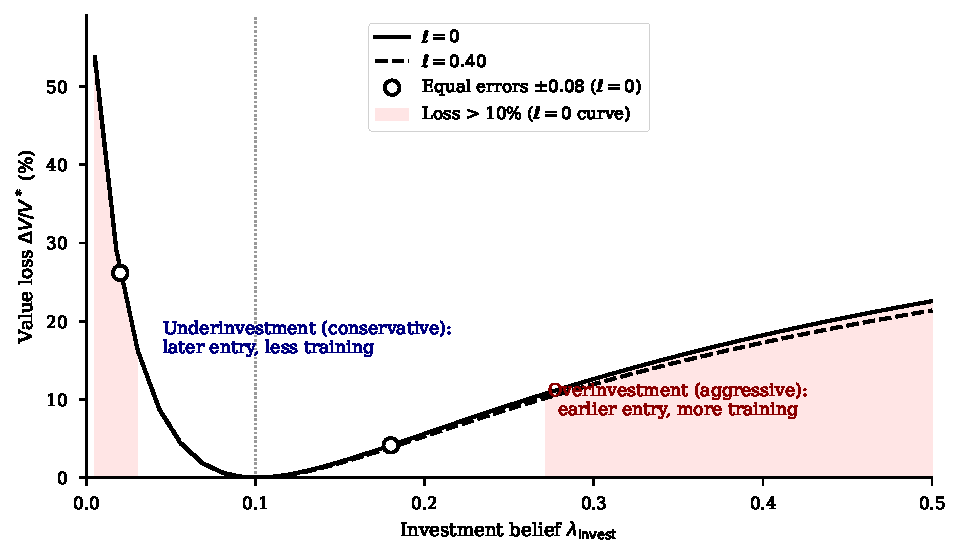
\includegraphics[keepaspectratio]{figures/fig_investment_dilemma.pdf}}

}

\caption{\label{fig-investment-dilemma}Value loss as a function of the
investment belief \(\lambda_{\text{invest}}\) (Numerical Finding 1). The
loss \(\Delta V\), expressed as a percentage of the first-best value
\(\text{NPV}(\lambda_{\text{true}}, \lambda_{\text{true}})\), is plotted
against the investment belief \(\lambda_{\text{invest}}\) over
\([0.005, 0.50]\) for a fixed \(\lambda_{\text{true}} = 0.10\). Solid
line: unlevered (\(\ell = 0\)); dashed line: levered (\(\ell = 0.40\)),
for which \(\text{NPV}\) denotes the value of the total claims
\(E + D - I(K^*)\) under the unlevered policy. The shaded region is
bounded above by the unlevered curve and marks the belief range over
which that curve exceeds a 10\% loss. The open circles mark the equal
additive errors \(\lambda_{\text{invest}} = 0.02\) and \(0.18\) on the
unlevered curve. Under- and overinvestment here mean later or earlier
entry and less or more training: capacity \(K^*\) is invariant to the
belief (Proposition 1), so no point on either curve involves over- or
under-building. Parameters: baseline calibration.}

\end{figure}%

\subsubsection{Implications}\label{implications}

Within the model, being too conservative (\(\Delta V \approx 26\%\) at
\(\lambda_{\text{invest}} = 0.02\)) costs far more than being too
aggressive (\(\Delta V \approx 6\%\) at
\(\lambda_{\text{invest}} = 0.20\)), so the aggressive investment
reported for frontier AI labs is consistent with value maximization
rather than requiring extreme optimism about \(\lambda\). The exercise
compares two point mismatches and averages over no prior, so it
establishes only that a firm weighing the two errors equally would find
the conservative one more costly; it illustrates rather than identifies
beliefs. The asymmetry also makes \emph{underinvestment} more
informative: a conservative firm allocating little to training either
holds genuinely pessimistic beliefs about \(\lambda\) or is subject to
one of the frictions described above, none of which the model contains.
At the scale of trillion-dollar commitments, however, absolute rather
than percentage losses can be existential, especially with leverage:
``there's no hedge on Earth that could stop me from going bankrupt''
\citep{amodei2026dwarkesh}.

The dilemma is a single-firm exercise. In the duopoly extension
(Internet Appendix E), a conservative firm faces an additional strategic
penalty: by investing later and training less, it cedes the leader
position to a well-calibrated rival and forfeits the monopoly-phase
rents that drive the preemption equilibrium (Proposition 3). The
underinvestment cost rises from 26\% to 38\% and the overinvestment cost
from 6\% to 17\%: competition raises both losses but narrows the ratio
from about 4.6 to about 2.2 (Table~\ref{tbl-duopoly-dilemma}).

\section{Discussion}\label{sec-discussion}

I take up the welfare consequences of preemption, the model's testable
predictions, its policy implications, and its limitations.

\subsection{Welfare and
Overinvestment}\label{welfare-and-overinvestment}

I do not solve a planner's problem, so the model characterizes no social
optimum; the benchmark it computes is the monopolist's policy. Against
that benchmark preemption accelerates entry: the leader enters strictly
earlier than a monopolist would (Proposition 3,
Figure~\ref{fig-competition-effect}), and the follower then enters to
preserve its contest share. Whether industry capacity exceeds what two
firms would install cooperatively, and so whether preemption dissipates
rents on net, requires a benchmark I do not compute.

\subsection{Testable Predictions}\label{testable-predictions}

The model generates four cross-sectional predictions, testable in
principle on the small cross-section of frontier AI labs; \(\hat{\phi}\)
is a firm's observed training fraction.

\begin{enumerate}
\def\labelenumi{\arabic{enumi}.}
\tightlist
\item
  Training has two faces in credit risk. The prediction on default
  probability is mediated by beliefs: a lab that trains more because it
  expects the switch sooner (higher \(\hat{\phi}\) revealing higher
  \(\lambda\), Section~\ref{sec-calibration}) should exhibit a
  \emph{lower default probability} conditional on leverage, capacity,
  and demand. Holding beliefs fixed, the comparison is local: more
  training lowers the default boundary only for \(\hat{\phi}\) below the
  allocation optimum, and raises it for \(\hat{\phi}\) above it. The
  prediction on recovery is unconditional: higher \(\hat{\phi}\) implies
  \emph{higher losses given default}, since the continuation value that
  sustains solvency is destroyed in bankruptcy. The net effect on
  spreads is ambiguous, so the sharper prediction is the decomposition,
  that training-heavy labs default less often but recover less when they
  do.
\item
  Firms with higher \(\hat{\phi}\) should have higher equity betas,
  under the auxiliary assumption, imported from
  \citet{aguerrevere2009real}, that the H-regime component of value
  carries the higher systematic-risk loading; the model itself discounts
  every claim at a single rate \(r\) and has no pricing kernel, so this
  is a conjecture about value composition rather than a model
  implication. Because composition here shifts with the
  training-inference split at a given capacity, \(\hat{\phi}\) should
  carry explanatory power beyond capacity and concentration measures.
\item
  Equity value is increasing but \emph{concave} in \(\lambda\) over the
  policy-relevant range (Section~\ref{sec-model},
  Figure~\ref{fig-lambda-option-value}), because the regime-switch
  option saturates, so within that range negative timeline news should
  reduce AI lab valuations by more than equally sized positive news
  increases them. The claim does not extend to the smallest arrival
  rates: below \(\lambda \approx 0.085\) the option value is convex in
  \(\lambda\), and below \(\lambda \approx 0.025\), where the optimal
  allocation falls under the faith-based survival threshold
  \(\underline{\phi}\), it \emph{decreases} in \(\lambda\) (Remark 3).
  The prediction is therefore silent about firms priced on very long
  timelines, and high-\(\hat{\phi}\) firms carry the larger exposure.
\item
  Training fractions should be explained by beliefs about AI timelines
  and technology parameters, not by competitive position: leader,
  follower, and monopolist all choose the same \(\phi^*\) (Proposition
  3(ii)). Order of entry should predict investment \emph{timing} and
  \emph{scale} but not, controlling for beliefs, the training-inference
  split.
\end{enumerate}

These predictions are directional, and the small cross-section currently
limits formal testing: recovery regressions using training-compute
proxies could test prediction 1, and event studies around capability
releases could test the asymmetric response.

\subsection{Policy Implications}\label{policy-implications}

The model bears on financial stability, competition policy, and
disclosure, though in each case it supports a narrower claim than the
policy question requires. On financial stability, irreversible
investment, leverage, and regime-dependent demand compress the firm's
margin of safety at entry (Section~\ref{sec-model},
Section~\ref{sec-valuation}), and the faith-based survival channel
(Proposition 2) makes solvency depend on a belief parameter, so at the
calibrated optimum, where \(\phi^* > \tilde{\phi}\), a downward revision
in \(\lambda\) would raise the default boundary and cut equity value
simultaneously; with no asset market and no feedback from liquidation
onto prices, the model cannot take the further step to fire sales or
contagion. On competition policy, preemption cuts the leader's trigger
well below the monopolist's (Section~\ref{sec-calibration}), so capacity
announcements are weak evidence about demand expectations: a firm racing
a rival and a firm expecting an early switch both enter early. On
disclosure, \(\phi\) jointly determines the default boundary and the
composition of firm value (Propositions 1 and 2), so an investor working
inside this model would need \(\hat{\phi}\), not compute spending alone,
to locate a lab relative to its default boundary.

\subsection{Limitations}\label{limitations}

The static training fraction is the model's sharpest simplification, and
a two-period extension in Internet Appendix E
(Table~\ref{tbl-dynamic-phi}) signs and bounds the resulting bias. The
bias is not a drift in the allocation over time, since the switch time
is exponential and the firm learns nothing from its non-arrival; it is
the value of the option to \emph{re-purpose} compute at the switch,
which biases the pre-switch allocation downward. The static model is the
polar case in which the whole H-regime prize must be bought in advance,
so its \(\phi^* \approx 0.70\) is an \emph{upper bound}. That exercise
solves allocation and value only, not default or belief mismatch, so
what it says about the headline mechanisms is a conjecture rather than a
result: the Proposition 2 solvency floor and the Numerical Finding 1
asymmetry both run through the \emph{level} of pre-switch training,
which the lower \(\phi_1\) would attenuate.

The training technology is stylized in four further respects. Training
earns no revenue in regime \(L\) and post-switch revenue requires no
inference capacity, a knife-edge that sharpens the allocation trade-off;
in practice inference demand likely remains large after the switch and
training raises pre-AGI revenue, which would attenuate it. Training is a
flow allocation of installed capacity rather than an accumulated stock
of capability, so there is no learning curve. Capacity is installed
once, as a single irreversible lump. Inference-time scaling also blurs
the training-inference boundary the model treats as sharp.

The arrival rate \(\lambda\) is exogenous. A natural extension would
make it a function of aggregate training compute. I do not solve it, and
what follows is a conjecture rather than a result: a decentralized
equilibrium would plausibly leave that spillover partly uninternalized,
so equilibrium training could fall short of what a coordinating industry
would choose, and the two forces would then run in opposite directions,
preemption toward overinvestment in capacity and the spillover toward
underinvestment in training.

Leverage is a stress-test parameter rather than an equilibrium financing
choice. \citet{leland1994corporate} assumes publicly traded equity and
continuously tradeable debt, whereas frontier AI labs reportedly finance
themselves with SAFE notes, convertible debt, and multi-class equity.
The mechanism is best read as a tractable approximation to the distress
risk these firms face: \(X_D\) is the demand level at which the firm can
no longer sustain operations, whether the binding constraint is a missed
coupon, a failed funding round, or a covenant violation. Par issuance at
\(r_c < r\) also implies a financing subsidy the model does not
endogenize.

Finally, the Tullock contest function is a reduced form that abstracts
from product differentiation, network effects, and switching costs, and
it omits the market-growing effect of AI adoption, which biases the
model toward stronger competition effects; the Cournot alternative is
discussed in Section~\ref{sec-duopoly} and Internet Appendix E. All
valuation uses the reduced-form risk-adjusted framework of
Section~\ref{sec-model} and Internet Appendix B, a certainty-equivalent
convention rather than a pricing measure, so physical default
probabilities would be lower.

\section{Conclusion}\label{sec-conclusion}

In this model of AI compute investment, capacity, timing, and the
training-inference split respond to different forces. In the single-firm
reduced model, optimal capacity is pinned down by the revenue and cost
technology and is invariant to beliefs about when AGI arrives, while the
training fraction is governed by beliefs about the arrival rate
\(\lambda\) (Proposition 1); under competition, the entry trigger is
compressed further by the threat of preemption (Proposition 3). That
separation is what makes belief errors asymmetric: a firm with the wrong
timeline installs the same capacity, and carries the same coupon, as a
firm with the right one, so the entire cost of the error runs through
the entry trigger and the training allocation.

Three tensions drive the results. The first is current cash flow against
future capability: firms balance inference revenue in regime \(L\),
which funds operations and services debt, against training whose payoff
arrives only in regime \(H\). The optimal training fraction \(\phi^*\)
increases in \(\lambda\), so more optimistic firms train more,
consistent with the archetypes in Section~\ref{sec-calibration}. The
second is growth-option upside against leverage and default risk. The
\emph{faith-based survival} channel holds at the calibrated optimum but
not throughout the parameter space: its \(A_{\text{eff}}\)-channel
threshold \(\underline{\phi} \approx 0.18\) lies well below
\(\phi^* \approx 0.70\), so at baseline a firm that trains more because
it expects the switch sooner sits further from default (Proposition 2).
At a fixed belief, by contrast, the boundary is U-shaped in the training
fraction with its minimum at \(\phi^*\), so training beyond the optimum
raises it, and the channel reverses for beliefs below
\(\lambda \approx 0.034\).

The third is the asymmetric cost of belief mismatches
(Section~\ref{sec-valuation}). Numerical Finding 1 shows that in this
calibration conservative underinvestment costs more in expected value
than aggressive overinvestment for the same belief error, because
under-allocating to training forfeits the option value of regime \(H\)
that dominates firm value. Overinvestment instead carries the higher
tail exposure: an aggressive firm enters at a lower trigger while
over-training depresses the regime-\(L\) revenue that services its debt,
leaving it closer to its default boundary at entry, with a five-year
default probability at \(\ell = 0.40\) of 5.04\% against 0.64\% at
correct beliefs (both no-switch upper bounds on the pre-switch
probability). This is not a general case for building more. Moderate
overinvestment is cheap, about 6\% of unlevered value at
\(\lambda_{\text{invest}} = 0.20\) against roughly 23\% at
\(\lambda_{\text{invest}} = 0.50\)
(Figure~\ref{fig-investment-dilemma}), and both percentages are those of
the reduced model: re-solving the piecewise stopping problem, with the
post-switch scale precommitted or unrestricted, preserves the ranking
but moves the magnitudes (Internet Appendix B). Commitments at the
extreme end are therefore more readily reconciled with genuinely
optimistic beliefs than with a low-cost posture, though the model
separates neither beliefs from signaling nor either from agency motives,
and the calibration is stylized.

The model abstracts from talent constraints, alignment objectives,
geopolitical competition, entrants such as DeepSeek
\citep{deepseek2025r1}, and a \$600 billion gap between AI
infrastructure spending and current AI revenue \citep{cahn2024gap} that
may discipline the race through financial markets before any of these
other forces do. Three extensions follow directly: dynamic learning
about \(\lambda\), dynamic reallocation, and financial frictions. The
central point is simpler than any of them. Training capacity buys a
continuation value that creditors cannot seize, so a firm that bets on
the switch survives on the strength of its belief and pays for it in
what it can pledge. That is why a wrong timeline belief is punished in
expected value when the firm is too cautious and in default risk when it
is too bold.

\newpage
\clearpage

\section*{References}\label{references}
\addcontentsline{toc}{section}{References}

\begingroup
\raggedright

\renewcommand{\bibsection}{}
\bibliography{references.bib}

\endgroup

\clearpage
\thispagestyle{empty}
\begin{center}
\vspace*{0.18\textheight}
{\Large\bfseries Internet Appendix for}\\[1.2em]
{\Large\bfseries ``Capacity, Training, and Default in the Race to Artificial General Intelligence''}\\[3em]
{\large\itshape Supplementary material intended for online publication as an e-companion}
\label{ia-cover}%
\end{center}

\clearpage
\setcounter{page}{1}
\setcounter{table}{0}
\setcounter{figure}{0}
\setcounter{equation}{0}
\renewcommand{\thetable}{IA\arabic{table}}
\renewcommand{\thefigure}{IA\arabic{figure}}
\renewcommand{\theequation}{IA\arabic{equation}}

\section*{Internet Appendix}\label{internet-appendix}
\addcontentsline{toc}{section}{Internet Appendix}

This Internet Appendix collects the proofs, numerical methods,
calibration sources, robustness exercises, and supporting exhibits
behind the main text. Internet Appendix A proves Propositions 1--3 and
records the analytical status of each result; the sections that follow
document the numerical verification methods (B), the calibration details
and data sources (C), the parameter sensitivity (D), and the robustness
exercises (E), and then present the single-firm illustrations (F), the
scale-gap diagnostic (G), and the credit-spread and default-probability
formulas (H) that the main text summarizes.

\subsection*{Parameters and Notation}\label{parameters-and-notation}
\addcontentsline{toc}{subsection}{Parameters and Notation}

Table~\ref{tbl-parameters} lists the model's parameters with their
baseline values and calibration status, and Table~\ref{tbl-notation}
defines the additional notation used throughout.

\begin{longtable}[]{@{}
  >{\centering\arraybackslash}p{(\linewidth - 8\tabcolsep) * \real{0.0800}}
  >{\raggedright\arraybackslash}p{(\linewidth - 8\tabcolsep) * \real{0.2000}}
  >{\centering\arraybackslash}p{(\linewidth - 8\tabcolsep) * \real{0.0800}}
  >{\raggedright\arraybackslash}p{(\linewidth - 8\tabcolsep) * \real{0.4600}}
  >{\centering\arraybackslash}p{(\linewidth - 8\tabcolsep) * \real{0.1000}}@{}}
\caption{Model parameters with baseline values and calibration status.
The rate parameters \(r\), \(\mu_L\), and \(\mu_H\) are risk-adjusted;
\(\sigma\) is common to the physical and risk-adjusted measures (see
Section~\ref{sec-model}). \(\phi\) is an endogenous choice variable,
while \(\ell\) is fixed exogenously and varied as a stress-test
parameter; ``n.a.'' indicates that the entry does not apply. Status:
``Inferred'' = backed out from observable proxies; ``Chosen'' = set to
generate plausible magnitudes without a precise empirical target;
``Standard'' = standard value from the
literature.}\label{tbl-parameters}\tabularnewline
\toprule\noalign{}
\begin{minipage}[b]{\linewidth}\centering
Symbol
\end{minipage} & \begin{minipage}[b]{\linewidth}\raggedright
Parameter
\end{minipage} & \begin{minipage}[b]{\linewidth}\centering
Baseline
\end{minipage} & \begin{minipage}[b]{\linewidth}\raggedright
Target / Source
\end{minipage} & \begin{minipage}[b]{\linewidth}\centering
Status
\end{minipage} \\
\midrule\noalign{}
\endfirsthead
\toprule\noalign{}
\begin{minipage}[b]{\linewidth}\centering
Symbol
\end{minipage} & \begin{minipage}[b]{\linewidth}\raggedright
Parameter
\end{minipage} & \begin{minipage}[b]{\linewidth}\centering
Baseline
\end{minipage} & \begin{minipage}[b]{\linewidth}\raggedright
Target / Source
\end{minipage} & \begin{minipage}[b]{\linewidth}\centering
Status
\end{minipage} \\
\midrule\noalign{}
\endhead
\bottomrule\noalign{}
\endlastfoot
\(\mu_L\) & L-regime drift (per year) & 0.01 & Cloud computing baseline
growth & Chosen \\
\(\mu_H\) & H-regime drift (per year) & 0.06 & Upper-range AI revenue
growth projections & Chosen \\
\(\sigma\) & Volatility (annualized) & 0.25 & Order of magnitude from
quarterly revenue volatility of cloud providers; no directly observable
counterpart to \(X\) & Chosen \\
\(r\) & Discount rate (WACC, per year) & 0.12 & WACC, representative
frontier AI lab & Inferred \\
\(\lambda\) & Arrival rate (per year) & 0.10 & Regime-switch arrival
rate (exogenous belief) & Chosen \\
\(\alpha\) & Revenue elasticity & 0.40 & Concavity motivated by
scaling-law compute-to-loss exponents (a loss exponent is not a revenue
elasticity); satisfies (A2) & Chosen \\
\(\gamma\) & Cost convexity & 1.50 & Power/supply-chain bottlenecks,
site prep costs & Chosen \\
\(c\) & Unit cost & 1.00 & Normalization & n.a. \\
\(\delta\) & Operating cost rate (per year) & 0.03 & Power, cooling,
maintenance (flow cost only); jointly normalized with the capacity unit
and \(c\) & Chosen \\
\(\phi\) & Training fraction & n.a. & Endogenous choice variable &
n.a. \\
\(\ell\) & Leverage ratio (debt / total capital) & n.a. & Exogenous
stress-test parameter, varied over \([0, 0.7]\) & n.a. \\
\(r_c\) & Coupon rate (per year) & 0.05 & Stylized cost of debt for
frontier AI labs; below \(r\), so debt is not fairly priced at issuance
(Section~\ref{sec-model}) & Inferred \\
\(b\) & Bankruptcy cost & 0.30 & Bankruptcy cost fraction & Standard \\
\end{longtable}

\begin{longtable}[]{@{}
  >{\centering\arraybackslash}p{(\linewidth - 4\tabcolsep) * \real{0.1200}}
  >{\raggedright\arraybackslash}p{(\linewidth - 4\tabcolsep) * \real{0.5800}}
  >{\raggedright\arraybackslash}p{(\linewidth - 4\tabcolsep) * \real{0.3000}}@{}}
\caption{Additional notation not listed in Table~\ref{tbl-parameters}.
``Derived (primitives)'' indicates quantities computed from exogenous
parameters only; ``Derived (choices)'' indicates quantities that
additionally depend on endogenous decisions
\((K, \phi)\).}\label{tbl-notation}\tabularnewline
\toprule\noalign{}
\begin{minipage}[b]{\linewidth}\centering
Symbol
\end{minipage} & \begin{minipage}[b]{\linewidth}\raggedright
Meaning
\end{minipage} & \begin{minipage}[b]{\linewidth}\raggedright
Type
\end{minipage} \\
\midrule\noalign{}
\endfirsthead
\toprule\noalign{}
\begin{minipage}[b]{\linewidth}\centering
Symbol
\end{minipage} & \begin{minipage}[b]{\linewidth}\raggedright
Meaning
\end{minipage} & \begin{minipage}[b]{\linewidth}\raggedright
Type
\end{minipage} \\
\midrule\noalign{}
\endhead
\bottomrule\noalign{}
\endlastfoot
\(X_t\) & Demand process & Exogenous (GBM) \\
\(K\) & Installed capacity & Endogenous (choice) \\
\(A_H\) & H-regime present-value multiplier: \(1/(r - \mu_H)\) & Derived
(primitives) \\
\(A_{\text{eff}}\) & Effective revenue coefficient combining L- and
H-regime values & Derived (choices) \\
\(\beta_H\) & Positive characteristic root, H-regime ODE & Derived
(primitives) \\
\(\beta_H^-\) & Negative characteristic root, H-regime ODE & Derived
(primitives) \\
\(\beta_L^+\) & Positive characteristic root, L-regime ODE (with
\(\lambda\)) & Derived (primitives) \\
\(\beta_L^-\) & Negative characteristic root, L-regime ODE (with
\(\lambda\)) & Derived (primitives) \\
\(B_H\) & Coefficient of the H-regime option value
\(F_H(X) = B_H X^{\beta_H}\) & Derived (choices) \\
\(C_D\) & Total coupon flow: \(C_D = r_c \, \ell \, I(K)\) & Derived
(choices) \\
\(\Omega\) & H-to-L present-value ratio setting \(\underline{\phi}\)
(\textbf{?@eq-phi-underbar}) & Derived (primitives) \\
\(s_i^L, s_i^H\) & Tullock contest shares (L-regime inference, H-regime
training) & Derived (choices) \\
\(X_D\) & Endogenous default boundary & Derived (choices) \\
\(X^*\) & Optimal investment trigger & Derived (choices) \\
\(X_L^{\text{mono}}\) & Leader's monopoly-only investment trigger (no
rival) & Derived (choices) \\
\(X_P\) & Preemption trigger & Derived (choices) \\
\(X_F^*\) & Follower's investment trigger & Derived (choices) \\
\(\Delta V\) & Value loss from belief mismatch (Numerical Finding 1) &
Derived (choices) \\
\(g\) & Scale-gap index (Internet Appendix G) & Derived (choices) \\
\end{longtable}

\newpage

\subsection*{A. Proofs and Supporting
Derivations}\label{a.-proofs-and-supporting-derivations}
\addcontentsline{toc}{subsection}{A. Proofs and Supporting Derivations}

The algebraic and single-variable-calculus content of Propositions 1--3
is machine-checked in Lean 4\footnote{\url{https://lean-lang.org/}} and
its mathematical library Mathlib. For Proposition 1, the formalization
covers the investment trigger Equation~\ref{eq-trigger-phi}, the net
present value at the trigger, the capacity first-order condition and its
closed-form solution \(K^*\), which does not depend on the training
fraction (Steps 1--4; the limit argument that makes this root the global
maximum is elementary calculus and is not formalized), and the reduction
of the training-fraction first-order condition to the unique interior
critical point \(\phi^*\) in closed form together with its comparative
statics (Steps 5--6). It also covers the reduction of the homogeneous
Euler ODE to the characteristic equation Equation~\ref{eq-beta-H} (a
power solution \(X^\beta\) solves the ODE if and only if
\(Q(\beta) = 0\)) and the sign, magnitude, and ordering of its roots,
namely \(\beta_H > 1\), \(\beta_L^- < 0\), and \(\beta_L^+ > \beta_H\).
For Proposition 2, it covers the quotient-rule derivative
\(\partial A_{\text{eff}}/\partial \lambda\), the faith-based survival
condition, the threshold \textbf{?@eq-phi-underbar}, the monotonicity of
the default boundary in leverage and rival capacity, and, for the exact
net threshold \(\tilde{\phi}\), the markup channel's monotonicity in
\(\lambda\) together with the net-condition rearrangement. For
Proposition 3, it covers the scale-invariance of the Tullock contest
share that underlies role-invariance, the separable reduction of the
follower's revenue coefficient, the contest-derivative factorization,
and the generic intermediate-value existence and strict-concavity
single-crossing lemmas underlying the preemption trigger \(X_P\),
conditional on the continuity, endpoint-sign, and (zero-leverage)
concavity hypotheses the paper supplies. Each theorem is proved in full,
depends only on the proof assistant's standard logical axioms, and is
stated for arbitrary admissible parameters rather than the baseline
calibration alone.

The scope is the algebra and calculus \emph{downstream} of the
optimal-stopping problem. The Hamilton--Jacobi--Bellman ODE
(Equation~\ref{eq-hjb-L}) and the value matching and smooth pasting
conditions are taken as given; conditional on them, the verification
establishes the reduction to the characteristic equation, the closed
forms, the first-order conditions, and the comparative statics that
follow. The stochastic-calculus derivation of the HJB equation itself,
and the optimal-stopping argument that the candidate value functions are
optimal, are not formalized; nor is the pure-power (\(A_1 = 0\)) form of
the L-regime option value, which is a solution convention rather than a
theorem (Step 5b below and Section~\ref{sec-conventions}). Results that
are numerical in nature, the magnitude of \(\tilde{\phi}\) and the
coupled-ODE, piecewise-stopping, and Dario's-dilemma computations
(Internet Appendix B), are likewise not formalized. The Lean proof
package accompanies the submission; the code reproducing the numerical
results (Python source, locked environment, and the commands behind each
exhibit) is in the public repository and will be archived with the paper
upon publication.

\subsubsection*{Proof of Proposition 1}\label{proof-of-proposition-1}
\addcontentsline{toc}{subsubsection}{Proof of Proposition 1}

\emph{Maintained assumptions.} The proof requires Assumption 1, in
particular conditions (A2)--(A4). It applies in the parameter region
where the paper adopts the simplified option value
\(F_L \propto X^{\beta_H}\) (condition A3; see Step 5b and
Section~\ref{sec-conventions}). The firm maximizes the option value
\(F(X_0) = (V(X^*, K, \phi) - I(K))(X_0/X^*)^{\beta_H}\) by choosing
\(X^*\), \(K\), and \(\phi\) jointly.

\emph{Step 1: Optimal trigger given \((K, \phi)\).} The value matching
and smooth pasting conditions yield: \[
X^*(K, \phi) = \frac{\beta_H}{\beta_H - 1} \cdot \frac{\delta K/r + cK^\gamma}{A_{\text{eff}}(\phi, K)},
\] where
\(A_{\text{eff}}(\phi, K) = [(1-\phi)K]^\alpha / (r - \mu_L + \lambda) + \lambda / (r - \mu_L + \lambda) \cdot (\phi K)^\alpha \cdot A_H\)
is the effective revenue coefficient.

\emph{Step 2: NPV at the trigger.} Define
\(\Theta(K) = cK^\gamma + \delta K / r\), the investment outlay plus the
present value of the operating-cost flow. The present value of revenue
at the trigger is
\(A_{\text{eff}} \cdot X^* = \frac{\beta_H}{\beta_H - 1} \Theta(K)\), so
the NPV at the trigger is: \[
V - I = \frac{1}{\beta_H - 1}\, \Theta(K).
\]

\emph{Step 3: Joint optimization over \((K, \phi)\).} Substituting the
trigger and NPV into \(F(X_0)\): \[
F(X_0) = \mathcal{C} \cdot \frac{A_{\text{eff}}(\phi, K)^{\beta_H}}{\Theta(K)^{\beta_H - 1}} \equiv \mathcal{C} \cdot h(K, \phi),
\] where
\(\mathcal{C} = \frac{1}{\beta_H - 1}\left(\frac{(\beta_H - 1) X_0}{\beta_H}\right)^{\beta_H} > 0\)
is independent of \((K, \phi)\). The optimal \((K^*, \phi^*)\) maximizes
\(h(K, \phi) = A_{\text{eff}}^{\beta_H} / \Theta^{\beta_H - 1}\).

\emph{Step 4: First-order condition for \(K\).} Setting
\((\partial \ln h / \partial K) = 0\):
\begin{equation}\protect\phantomsection\label{eq-foc-K}{
\frac{\beta_H}{A_{\text{eff}}} \frac{\partial A_{\text{eff}}}{\partial K} = \frac{(\beta_H - 1)(c\gamma K^{\gamma - 1} + \delta / r)}{cK^\gamma + \delta K / r}.
}\end{equation} Since \(A_{\text{eff}}\) takes the form
\(g(\phi) \cdot K^\alpha\) (both in the pure H-regime and under regime
switching), the left-hand side reduces to \(\alpha \beta_H / K\), which
is independent of \(\phi\). Solving for \(K\) yields the closed-form
expression in Proposition 1, confirming that \(K^*\) depends only on the
cost and technology parameters
\((\alpha, \beta_H, \gamma, \delta, r, c)\), not on the training
fraction. The critical point is the global maximum. At fixed \(\phi\),
\(h \propto K^{\alpha\beta_H} / (cK^\gamma + \delta K/r)^{\beta_H - 1}\)
is continuous and strictly positive on \((0, \infty)\). As \(K \to 0\)
the linear term dominates the denominator and
\(h \sim K^{\alpha\beta_H - (\beta_H - 1)} \to 0\), because the upper
bound in (A2) gives \(\alpha\beta_H > \beta_H - 1\). As \(K \to \infty\)
the convex term dominates and
\(h \sim K^{\alpha\beta_H - \gamma(\beta_H - 1)} \to 0\), because the
lower bound in (A2) gives \(\alpha\beta_H < \gamma(\beta_H - 1)\). A
positive continuous function vanishing at both ends attains an interior
maximum, and Equation~\ref{eq-foc-K} is linear in \(K^{\gamma - 1}\)
with a single root, so that root is it. Both limits require
\(\delta > 0\): at \(\delta = 0\) the denominator is \(cK^\gamma\)
alone, \(h \sim K^{\alpha\beta_H - \gamma(\beta_H - 1)}\) is
monotonically decreasing on the whole half-line, and no interior optimum
exists (the closed form returns \(K^* = 0\)), which is why (A1) imposes
\(\delta > 0\).

\emph{Step 5: Existence of interior \(\phi^*\).}

Write
\(A_{\text{eff}}(\phi) = w_L \cdot [(1-\phi)K]^\alpha + w_H \cdot (\phi K)^\alpha\),
where \(w_L = 1/(r - \mu_L + \lambda) > 0\) and
\(w_H = \lambda A_H / (r - \mu_L + \lambda) > 0\). Since \(\Theta(K)\)
is independent of \(\phi\), maximizing \(h\) over \(\phi\) is equivalent
to maximizing \(A_{\text{eff}}(\phi)\).

The first derivative with respect to \(\phi\) is: \[
\frac{\partial A_{\text{eff}}}{\partial \phi} = \alpha K^\alpha \bigl[-w_L (1-\phi)^{\alpha - 1} + w_H \phi^{\alpha - 1}\bigr].
\]

\emph{Boundary behavior.} Since \(\alpha \in (0,1)\), the exponent
\(\alpha - 1 < 0\), so:

\begin{itemize}
\tightlist
\item
  As \(\phi \to 0^+\): \(\phi^{\alpha - 1} \to +\infty\) while
  \((1-\phi)^{\alpha-1} \to 1\), so
  \(\partial A_{\text{eff}}/\partial \phi \to +\infty\). (Inada
  condition: the first unit of training has infinite marginal value.)
\item
  As \(\phi \to 1^-\): \((1-\phi)^{\alpha - 1} \to +\infty\) while
  \(\phi^{\alpha-1} \to 1\), so
  \(\partial A_{\text{eff}}/\partial \phi \to -\infty\). (Inada
  condition: the first unit of inference has infinite marginal value.)
\end{itemize}

Since \(\partial A_{\text{eff}}/\partial \phi\) is continuous on
\((0,1)\), positive near \(\phi = 0\), and negative near \(\phi = 1\),
by the intermediate value theorem there exists \(\phi^* \in (0,1)\) with
\(\partial A_{\text{eff}}/\partial \phi = 0\).

\emph{Uniqueness.} The second derivative is: \[
\frac{\partial^2 A_{\text{eff}}}{\partial \phi^2} = \alpha(\alpha - 1) K^\alpha \bigl[w_L (1-\phi)^{\alpha - 2} + w_H \phi^{\alpha - 2}\bigr] < 0
\] for all \(\phi \in (0,1)\), since \(\alpha \in (0,1)\) implies
\(\alpha(\alpha-1) < 0\) while both bracketed terms
\((1-\phi)^{\alpha - 2}\) and \(\phi^{\alpha - 2}\) are positive. Strict
concavity of \(A_{\text{eff}}\) in \(\phi\) guarantees uniqueness.

\emph{Interior solution.} Setting
\(\partial A_{\text{eff}} / \partial \phi = 0\) yields: \[
\frac{w_H}{w_L} = \left(\frac{1-\phi^*}{\phi^*}\right)^{\alpha - 1},
\] which uniquely determines \(\phi^*\) as an increasing function of
\(w_H / w_L\).

\emph{Step 6: Comparative statics.} Because \(A_{\text{eff}}\) is
strictly concave in \(\phi\) with interior maximizer \(\phi^*\), and
\(\phi^*\) is increasing in \(w_H/w_L\) (Step 5):

\begin{enumerate}
\def\labelenumi{(\roman{enumi})}
\tightlist
\item
  \(\partial \phi^* / \partial \lambda > 0\): Higher \(\lambda\)
  increases \(w_H / w_L = \lambda A_H\). Since \(\phi^*\) is increasing
  in \(w_H / w_L\), the optimal training fraction rises. (ii)
  \(\partial \phi^* / \partial \mu_H > 0\): Higher \(\mu_H\) lowers
  \(r - \mu_H\), increasing \(w_H / w_L = \lambda / (r - \mu_H)\). Since
  \(\phi^*\) is increasing in \(w_H / w_L\), the optimal training
  fraction rises. Note that \(\phi^*\) is independent of \(\mu_L\): both
  \(w_L = 1/(r - \mu_L + \lambda)\) and
  \(w_H = \lambda A_H / (r - \mu_L + \lambda)\) share the denominator
  \((r - \mu_L + \lambda)\), so
  \(w_H / w_L = \lambda A_H = \lambda / (r - \mu_H)\) does not depend on
  \(\mu_L\). \(\square\)
\end{enumerate}

\emph{Step 5b: The pure-power form of \(F_L\) (solution convention).}

This block justifies the option-value form assumed in Step 1; it is
placed after the proof rather than interrupting it.

The general L-regime option value
\(F_L(X) = A_1 X^{\beta_L^+} + \Gamma X^{\beta_H}\)
(Equation~\ref{eq-option-L-general}) decomposes into a homogeneous
component \(A_1 X^{\beta_L^+}\), where \(\beta_L^+\) is the positive
root of the homogeneous L-regime switching ODE (hazard-adjusted discount
rate \(r + \lambda\); Equation~\ref{eq-hjb-L} without its forcing term
\(\lambda B_H X^{\beta_H}\)), and a particular component
\(\Gamma X^{\beta_H}\), driven by the forcing term \(\lambda F_H(X)\),
with coefficient \(\Gamma = -\lambda B_H / Q_L(\beta_H)\) determined by
the ODE (Equation~\ref{eq-particular-C}). The coefficient is positive:
evaluating \(Q_L\) at the H-regime root gives
\(Q_L(\beta_H) = (\mu_L - \mu_H)\beta_H - \lambda < 0\), which also
places \(\beta_H\) strictly below the larger root \(\beta_L^+\), since
\(Q_L\) is an upward parabola. Two qualifications bear on this
decomposition; the second is the substantive one.

\emph{Range of validity of the forcing term.} The forcing term
\(\lambda F_H(X)\) takes the option form \(\lambda B_H X^{\beta_H}\)
only for \(X < X_H^*\). For \(X > X_H^*\) a switch to the H-regime is
followed by immediate exercise, so the forcing term is the exercised
value. At the scale \(K_H^*\) chosen for entry at \(X_H^*\) it is
\(\lambda [V_H(X, K_H^*, \phi_H^*) - I(K_H^*)]\), affine in \(X\); a
firm that has not invested when the switch arrives is not bound to that
scale, and its payoff is the envelope
\(\lambda \max_K [V_H(X, K, \phi_H^*) - I(K)]\), which is tangent to the
affine payoff at \(X_H^*\) and lies above it for \(X > X_H^*\) (by
13.6\% at \(X = 2X_H^*\) at baseline). In either case the continuation
value solves a piecewise problem with value and slope matched at
\(X_H^*\); Internet Appendix B solves the precommitted-scale version in
closed form and the unrestricted version numerically. Accordingly,
Equation~\ref{eq-particular-C} is the exact particular solution on
\((0, X_H^*)\); on \((X_H^*, X^*)\) the pure power form extends it. At
the baseline calibration \(X^* \approx 0.0047\) exceeds
\(X_H^* \approx 0.0028\), so this interval is non-empty.

\emph{Sign of the homogeneous coefficient.} The homogeneous term is the
value of being able to exercise \emph{before} the regime switch, using
the combined revenue coefficient. Assumption (A3) does not eliminate it.
What (A3) rules out is an interior optimal \emph{scale} for the
standalone, no-switching L-regime problem: at a fixed capacity \(K\)
that problem has the finite trigger
\(X_L^{\text{pure}}(K) = [\beta_L^0/(\beta_L^0 - 1)] \cdot [\delta K/r + I(K)]/(A_L K^\alpha)\)
with \(A_L = 1/(r - \mu_L)\) and \(\beta_L^0 \approx 2.33\) the positive
root of the characteristic equation discounted at \(r\) (no switching),
and an interior optimum over \(K\) requires the option premium ratio
\((1 - 1/\beta_L^0)/\alpha < 1\) (the L-regime analogue of condition
(A2): the marginal value of capacity, \(\alpha\), must be large enough
relative to the markup-adjusted payout share). At baseline that ratio is
\(1.43\), and the hazard-adjusted version in (A3),
\(\Phi_L = (1 - 1/\beta_L^+)/\alpha \approx 1.67\) with \(\beta_L^+\)
the root at \(r + \lambda\), is larger still; either way the standalone
L-regime scale problem has no interior optimum. That is a statement
about the absence of an optimal scale, not about profitability: small
standalone L-regime projects have positive value at positive demand, and
the option factor diverges as \(K \to 0\), which is exactly why no scale
is optimal. It does not follow that the coefficient on the homogeneous
root vanishes. Nor can the sign be settled by the replication argument
that suggests itself, namely that the firm can always follow the pure
switching strategy (never exercise in regime \(L\), wait for the
H-regime arrival, and then hold the H-regime option) and that this
strategy is worth \(\Gamma X^{\beta_H}\). It is not: the pure switching
strategy faces the same piecewise forcing as every other strategy, so
its value is \(A_w X^{\beta_L^+} + \Gamma X^{\beta_H}\) below \(X_H^*\)
and
\(G_w X^{\beta_L^-} + [\lambda p_H/(r + \lambda - \mu_L)] X - \lambda q_H/(r + \lambda)\)
above it, where \(p_H\) and \(q_H\) are the slope and intercept of the
exercised H-regime payoff (Internet Appendix B) and \((A_w, G_w)\) are
pinned by value and slope matching at \(X_H^*\) once the no-bubble
condition removes \(X^{\beta_L^+}\) from the upper branch. The exercised
H-regime payoff lies strictly below the extrapolated power
\(B_H X^{\beta_H}\) for \(X > X_H^*\), since the two are tangent at
\(X_H^*\) and the power is convex, so the true forcing is dominated
pointwise by the forcing Equation~\ref{eq-particular-C} assumes, and
\(A_w < 0\): at the baseline calibration
\(A_w \approx -1.18 \times 10^4\), so the pure switching value lies
\emph{below} \(\Gamma X^{\beta_H}\) everywhere on \((0, X_H^*)\), by
10\% at \(X = X_H^*\). The valid statements are therefore that
\(A_1 > A_w\), since exercising before the switch is worth something,
and that \(\Gamma X^{\beta_H}\) is an upper, not a lower, bound on the
precommitted-scale continuation value below \(X_H^*\), the latter
because the extrapolated forcing dominates the true one pointwise and,
at the baseline calibration, the fictitious problem with that forcing
has no finite exercise boundary at all (Internet Appendix B). Solving
the precommitted-scale piecewise problem numerically (Internet Appendix
B) gives \(A_1 \approx -1.01 \times 10^4 < 0\) at baseline. Neither
\(A_1 = 0\) nor \(A_1 \geq 0\) can be derived from (A3). At the baseline
calibration, \(\beta_L^+ \approx 3.01\) gives \(\Phi_L \approx 1.67\),
so (A3) holds with a wide margin.

\emph{The convention.} I nonetheless impose \(A_1 = 0\), and price the
pre-investment option with the pure power form
\(F_L(X) \propto X^{\beta_H}\) on the whole continuation region
\((0, X^*)\). This is the unconditional-\(A_{\text{eff}}\) convention of
Section~\ref{sec-conventions}: option-like L-regime payoffs are
discounted with the H-regime exponent \(\beta_H\) rather than with a
regime-switching first-passage factor mixing \(X^{\beta_L^+}\) and
\(X^{\beta_H}\), and the exercise payoff is the unconditional L-regime
installed value. With a single power in the continuation region,
dividing value-matching by smooth pasting at the investment trigger
\(X^*\) eliminates the coefficient and yields: \[
X^* = \frac{\beta_H}{\beta_H - 1} \cdot \frac{\delta K^*/r + I(K^*)}{A_{\text{eff}}(\phi^*, K^*)},
\] confirming Equation~\ref{eq-trigger-phi}. The trigger depends only on
the value-matching/smooth-pasting ratio, not on the level of the
coefficient, which value-matching at \(X^*\) then determines; the two
boundary conditions therefore pin down the trigger and the level
jointly, and the system is exactly determined. The price of the
convention is that this smooth-fit level differs from the forced-ODE
value \(\Gamma\) of Equation~\ref{eq-particular-C}: at the baseline
calibration the smooth-fit coefficient is
\([V(X^*, K^*, \phi^*) - I(K^*)]/(X^*)^{\beta_H} \approx 16.5\) against
\(\Gamma \approx 21.1\). The direction of the resulting error is not
implied by that comparison, and I therefore solve the piecewise
free-boundary problem numerically and report the bias in Internet
Appendix B. At the baseline calibration the precommitted-scale
continuation value exceeds the convention's smooth-fit value at every
demand level while remaining below \(\Gamma X^{\beta_H}\), so the
convention understates the pre-investment option value, by 19\% at
\(X_0 = X^*/2\). The ordering is not general: it reverses for
\(\lambda \leq 0.02\). Propositions 1--3 are exact statements about the
model these conventions define. The verification exercise shows what
transfers to the exact problem and what does not: the levels of \(X^*\)
and \(K^*\) are properties of the reduced model rather than estimates of
the exact optimum, whereas the training fraction \(\phi^*\) is
numerically identical across the problems, and the value delivered by
the reduced-form policy is within about 3\% of the optimum among
policies that precommit the post-switch scale and within about 7\% of
the unrestricted optimum, which at baseline does not invest before the
switch at all (Internet Appendix B).

\subsubsection*{Proof of Proposition 2}\label{proof-of-proposition-2}
\addcontentsline{toc}{subsubsection}{Proof of Proposition 2}

\emph{Maintained assumptions.} Assumption 1(A1). Capacity
\((K_i, \phi_i)\) and rival \((K_j, \phi_j)\) are fixed at their optimal
values. The default boundary follows from the
\citet{leland1994corporate} framework adapted to regime switching.

\emph{One-way coupling and the single-boundary reduction.} In a general
regime-switching credit model, equity values \((E_L, E_H)\) satisfy
coupled ODEs with potentially regime-contingent default boundaries
\((X_D^L, X_D^H)\). One feature of the model and one approximation
together permit a tractable single-boundary reduction.

The feature is that the regime switch is absorbing (\(L \to H\) only, no
\(H \to L\)), so the H-regime equity \(E_H(X)\) satisfies a standard
(uncoupled) Leland ODE with revenue coefficient
\(A_H (\phi_i K_i)^\alpha s_i^H\) and closed-form solution
\(E_H(X) = A_H (\phi_i K_i)^\alpha s_i^H X - (C_D + \delta K_i)/r + D_H X^{\beta_H^-}\),
whose last term is the default option (put-like, with \(\beta_H^- < 0\)
and \(D_H > 0\)). The L-regime equity \(E_L(X)\) is then forced by
\(\lambda E_H(X)\), a one-way coupling.

The approximation is to replace \(E_H\) with its perpetuity component:
\[
E_H(X) \approx A_H (\phi_i K_i)^\alpha \cdot s_i^H \cdot X - C_D/r - \delta K_i/r,
\] after which the L-regime equity ODE yields a particular solution with
coefficient \(A_{\text{eff},i}\), and Leland's smooth pasting gives the
default boundary below in closed form. The omitted term
\(D_H X^{\beta_H^-}\) is the (positive) value of the H-regime default
option, so the perpetuity approximation understates the H-regime
continuation value and the closed-form boundary weakly \emph{overstates}
\(X_D\). The magnitude of the bias is computed by solving the coupled
system exactly: substituting the closed-form \(E_H\) (including
\(D_H X^{\beta_H^-}\)) into the L-regime ODE yields an additional
particular term \(C_2 X^{\beta_H^-}\) with
\(C_2 = -\lambda D_H / Q_L(\beta_H^-)\), and value matching plus smooth
pasting at \(X_D\) then determine the boundary jointly with the
homogeneous coefficient. At the baseline calibration the closed-form
boundary exceeds the coupled-system boundary by approximately 3\%,
uniformly across leverage levels (Internet Appendix B). The
approximation therefore errs against the faith-based survival mechanism,
making the levered firm look slightly riskier than the coupled system
implies, and is conservative for the credit-risk conclusions.

In the L-regime, the going-concern equity \(E(X)\) of
Equation~\ref{eq-equity} satisfies an ODE analogous to
Equation~\ref{eq-hjb-L}, with the firm defaulting when \(E(X_D) = 0\)
and \(E'(X_D) = 0\) (smooth pasting); the sunk equity contribution
enters the entry NPV \(E(X) - (1-\ell)I(K)\) but not the boundary
conditions. The resulting default boundary is: \[
X_D = \frac{\beta_L^-}{\beta_L^- - 1} \cdot \frac{C_D/r + \delta K_i/r}{A_{\text{eff},i}},
\] where \(\beta_L^-\) is the negative characteristic root,
\(C_D = r_c \cdot \ell \cdot I(K)\) is the coupon, and all comparative
statics below hold \emph{with \((K_i, \phi_i)\) fixed at their optimal
values}.

\emph{(i) Default boundary increasing in leverage.} \(X_D\) depends on
\(\ell\) only through the numerator via
\(C_D = r_c \cdot \ell \cdot I(K)\), which is strictly increasing in
\(\ell\). Since \(A_{\text{eff},i}\) is independent of \(\ell\) (holding
capacity and training fixed), \(\partial X_D / \partial \ell > 0\).

\emph{(ii) Default boundary decreasing in \(\lambda\) (faith-based
survival).} Holding \((K_i, \phi_i, K_j, \phi_j)\) fixed, define the
L-regime revenue flow
\(\Pi_L \equiv [(1-\phi_i)K_i]^\alpha \cdot s_i^L\) and the H-regime
revenue present value
\(\Pi_H \equiv (\phi_i K_i)^\alpha \cdot s_i^H / (r - \mu_H)\), both
positive. The effective revenue coefficient is: \[
A_{\text{eff},i} = \frac{\Pi_L + \lambda \cdot \Pi_H}{r - \mu_L + \lambda}.
\] Differentiating with respect to \(\lambda\): \[
\frac{\partial A_{\text{eff},i}}{\partial \lambda} = \frac{\Pi_H(r - \mu_L) - \Pi_L}{(r - \mu_L + \lambda)^2}.
\] This is positive whenever \(\Pi_H(r - \mu_L) > \Pi_L\), i.e., when
the H-regime revenue present value scaled by the L-regime net discount
rate \(r - \mu_L\) exceeds the L-regime revenue flow:
\begin{equation}\protect\phantomsection\label{eq-faith-condition}{
\frac{(\phi_i K_i)^\alpha \cdot s_i^H}{r - \mu_H} \cdot (r - \mu_L) > [(1-\phi_i)K_i]^\alpha \cdot s_i^L.
}\end{equation} Since \(\mu_H > \mu_L\) implies
\((r - \mu_L)/(r - \mu_H) > 1\), the factor \((r - \mu_L)\) amplifies
the H-regime term, making the condition easier to satisfy. Intuitively,
the condition requires that the training fraction \(\phi_i\) is large
enough that the H-regime continuation value contributes meaningfully to
\(A_{\text{eff},i}\).

\emph{Closed-form threshold (symmetric duopoly).} In the symmetric case
with \(s_i^L = s_i^H = 1/2\) and equal capacity, the contest shares and
\(K^\alpha\) terms cancel, and the condition reduces to
\((r - \mu_L)/(r - \mu_H) \cdot \phi^\alpha > (1-\phi)^\alpha\), i.e.,
\((\phi/(1-\phi))^\alpha > (r-\mu_H)/(r-\mu_L)\). Solving for \(\phi\):
\[
\phi > \underline{\phi} = \frac{\Omega}{1 + \Omega}, \quad \Omega = \left(\frac{r - \mu_H}{r - \mu_L}\right)^{1/\alpha}.
\] For the baseline calibration (\(r = 0.12\), \(\mu_H = 0.06\),
\(\mu_L = 0.01\), \(\alpha = 0.40\)):
\(\Omega = (0.06/0.11)^{2.5} \approx 0.22\), giving
\(\underline{\phi} \approx 0.18\).

\emph{Markup channel.} To complete the proof, note that \(X_D\) also
depends on \(\lambda\) through the markup factor
\(M(\beta_L^-) \equiv \beta_L^- / (\beta_L^- - 1)\), since \(\beta_L^-\)
is the negative root of
\(\tfrac{1}{2}\sigma^2 \beta(\beta - 1) + \mu_L \beta - (r + \lambda) = 0\)
and thus depends on \(\lambda\). The full derivative decomposes into two
opposing channels: \[
\frac{\partial X_D}{\partial \lambda} = \underbrace{\frac{\partial M}{\partial \lambda} \cdot \frac{N}{A_{\text{eff},i}}}_{>0\;\text{($\beta$-channel)}} + \underbrace{M(\beta_L^-) \cdot N \cdot \frac{\partial (1/A_{\text{eff},i})}{\partial \lambda}}_{<0\;\text{($A_{\text{eff}}$-channel)}},
\] where \(N = C_D/r + \delta K_i/r > 0\). The \(\beta\)-channel is
positive because increasing \(\lambda\) raises the hazard-adjusted
discount rate \((r + \lambda)\), making \(\beta_L^-\) more negative and
pushing the markup \(M\) toward 1 from below (since \(\beta_L^- < 0\)
implies \(M \in (0,1)\)):
\(dM/d\lambda = 1/[(\beta_L^- - 1)^2 \mathcal{R}] > 0\), where
\(\mathcal{R} = \sqrt{(\mu_L - \sigma^2/2)^2 + 2\sigma^2(r+\lambda)}\)
is the discriminant of the L-regime characteristic equation. The
\(A_{\text{eff}}\)-channel is negative under
Equation~\ref{eq-faith-condition}.

\emph{Exact net threshold.} The net sign resolves in closed form. In log
form,
\(\partial \ln X_D / \partial \lambda = m - \partial \ln A_{\text{eff},i} / \partial \lambda\),
where the markup semi-elasticity is
\(m \equiv (\mathrm{d}M/\mathrm{d}\lambda)/M = 1/[\beta_L^-(\beta_L^- - 1)\mathcal{R}] > 0\),
and, from the derivative above, \[
\frac{\partial \ln A_{\text{eff},i}}{\partial \lambda} = \frac{\Pi_H(r - \mu_L) - \Pi_L}{(\Pi_L + \lambda \Pi_H)\,\Delta}, \qquad \Delta \equiv r - \mu_L + \lambda,
\] with \(\Delta\) the hazard-adjusted net discount rate of the
L-regime. The condition \(\partial X_D / \partial \lambda < 0\) is
therefore \(\Pi_H(r - \mu_L) - \Pi_L > m(\Pi_L + \lambda \Pi_H)\Delta\),
which is \emph{linear} in \((\Pi_L, \Pi_H)\) and rearranges to \[
\frac{\Pi_H}{\Pi_L} > \frac{1 + m\Delta}{(r - \mu_L) - m\lambda\Delta},
\] provided the regularity condition \((r - \mu_L) > m\lambda\Delta\)
holds (it does throughout the calibration ranges; if it fails, no
allocation can deliver \(\partial X_D/\partial\lambda < 0\)). With
symmetric shares,
\(\Pi_H/\Pi_L = (\phi/(1-\phi))^\alpha / (r - \mu_H)\), giving the exact
threshold \(\tilde{\phi}\) of \textbf{?@eq-phi-tilde}. Since \(m > 0\),
\(\tilde{\Omega} > \Omega\) and \(\tilde{\phi} > \underline{\phi}\); as
\(m \to 0\) (no markup channel), \(\tilde{\phi} \to \underline{\phi}\).
At the baseline calibration \(m \approx 0.77\) and
\(\tilde{\phi} \approx 0.32\), between \(\underline{\phi} \approx 0.18\)
and \(\phi^* \approx 0.70\); the numerically measured \(\beta\)-channel
is about one-third of the \(A_{\text{eff}}\)-channel at \(\phi^*\),
consistent with the closed form. The sign flip of
\(\partial X_D/\partial \lambda\) at \(\tilde{\phi}\) is verified by
finite differences.

\emph{Sign at the optimal allocation.} Because \(\tilde{\phi}\) depends
on \(\lambda\) while \(\phi^*(\lambda)\) is increasing in \(\lambda\)
(Proposition 1), the comparison
\(\phi^*(\lambda) \gtrless \tilde{\phi}(\lambda)\) determines the sign
of \(\partial X_D/\partial \lambda\) at the optimum. At the baseline
calibration the two cross at \(\bar{\lambda} \approx 0.034\): for
\(\lambda > \bar{\lambda}\) (including the baseline \(\lambda = 0.10\)
and the full range used in Proposition 3(v)), \(\phi^* > \tilde{\phi}\)
and the default boundary falls with optimism; for
\(\lambda < \bar{\lambda}\), the optimal allocation is too
inference-heavy and \(X_D\) is locally \emph{increasing} in \(\lambda\)
at the optimum, a refinement that the closed form makes visible and that
finite-difference checks confirm (e.g., at \(\lambda = 0.02\),
\(\phi^* \approx 0.14 < \tilde{\phi} \approx 0.27\) and
\(\partial X_D/\partial\lambda > 0\)).

\emph{(iii) Leverage-training substitution.} Write the default boundary
as \(X_D = \Psi(\ell) / A_{\text{eff},i}(\phi_i)\), where
\(\Psi(\ell) = [\beta_L^- / (\beta_L^- - 1)] \cdot (r_c \ell I(K) / r + \delta K/r)\)
is strictly increasing in leverage (note: \(\Psi\) absorbs the markup
factor \(M\), unlike the cost term \(N\) in the
\(\lambda\)-decomposition above). In the monopoly and common-allocation
cases the contest shares are constant in \(\phi_i\), so
\(A_{\text{eff},i}(\phi_i)\) is the single-firm coefficient of
Proposition 1 (Step 5) up to a positive factor: strictly concave in
\(\phi_i\) with the interior maximizer \(\phi^*\), increasing on
\((0, \phi^*)\) and decreasing on \((\phi^*, 1)\). Against a rival at a
different allocation the shares \(s_i^L\) and \(s_i^H\) themselves
depend on \(\phi_i\), and Step 5 does not apply: the coefficient remains
single-peaked numerically, but its maximizer moves with the rival's
allocation (at equal baseline capacities under the Tullock contest, from
about \(0.84\) when \(\phi_j = 0.10\) to \(0.60\) when
\(\phi_j = 0.95\); under the arithmetic-mean industry-revenue benchmark
of Internet Appendix E it is \(\phi^*\) for every \(\phi_j\)). Part
(iii) is therefore stated relative to the maximizer of
\(A_{\text{eff},i}(\cdot)\) given \((K_j, \phi_j)\), which is \(\phi^*\)
in the symmetric and monopoly cases. For \(\phi_i < \phi^*\), a firm can
maintain a given default boundary \(X_D\) while increasing leverage
\(\ell\) (raising the numerator) by simultaneously increasing training
allocation \(\phi_i\) (raising \(A_{\text{eff},i}\) in the denominator).
For \(\phi_i > \phi^*\), the relationship reverses: further increases in
\(\phi_i\) would \emph{lower} \(A_{\text{eff},i}\) and \emph{raise} the
default boundary, so no such substitution is available. The economically
relevant range lies below the maximizer (baseline
\(\phi^* \approx 0.70\) in the symmetric case), where the substitution
applies. Note that this is a \emph{mechanical} relationship describing
the iso-\(X_D\) locus, not a statement about optimality: higher \(\phi\)
sacrifices L-regime revenue, and the net effect on equity value is
ambiguous. Leverage affects the firm through the coupon obligation
(numerator), while training allocation affects the firm through the
expected revenue (denominator).

\emph{(iv) Default boundary increasing in rival capacity.} Both contest
shares
\(s_i^L = [(1-\phi_i)K_i]^\alpha / \sum_j [(1-\phi_j)K_j]^\alpha\) and
\(s_i^H = (\phi_i K_i)^\alpha / \sum_j (\phi_j K_j)^\alpha\) are
decreasing in \(K_j\) (holding \(K_i\) fixed). Since
\(A_{\text{eff},i}\) is increasing in both contest shares,
\(\partial A_{\text{eff},i} / \partial K_j < 0\), and
\(\partial X_D / \partial K_j > 0\): stronger rivals raise the default
boundary. \(\square\)

\subsubsection*{Proof of Proposition 3}\label{proof-of-proposition-3}
\addcontentsline{toc}{subsubsection}{Proof of Proposition 3}

\emph{Maintained assumptions.} Assumption 1(A1)--(A2) and the four
solution conventions of Section~\ref{sec-conventions}, which are also
collected immediately before the statement of Proposition 3. Throughout
this proof \(F\) denotes the follower's option value, not the
single-firm option value of Proposition 1. Part (i) separates existence
(analytical, conditional on a computationally verified endpoint sign)
from uniqueness (analytical at \(\ell = 0\), computational for
\(\ell > 0\)). Part (ii) establishes an exact critical point
analytically and confirms global optimality computationally. Parts
(iii)--(v) are numerical findings, established by the computations
described in Internet Appendix B.

\emph{Part (i): Existence of \(X_P\) (conditional analytical).} The
argument follows \citet{huisman2015strategic}, Theorem 1, applied to the
enriched payoff functions incorporating training allocation and default
risk. I verify that continuity holds for the enriched model and that one
of the two required boundary conditions holds analytically; the other,
the upper-endpoint sign, is verified computationally.

\emph{Definitions.} Define \(L(X)\) as the leader's NPV of entering at
demand state \(X\): \(L(X) = E_L(X) - (1 - \ell)I(K_L)\), where
\(E_L(X)\) is the going-concern equity value of the leader's installed
project (which accounts for monopoly revenue until follower entry, then
duopoly revenue, plus the H-regime continuation value and the default
option). This is the equity convention of Section~\ref{sec-model}:
limited liability floors \(E_L\), not \(L\), so \(L\) inherits the
strictly negative constant \(-(1-\ell)I(K_L)\) wherever the
going-concern claim is worthless. Throughout, the leader's
\((K_L, \phi_L)\) is held at the monopoly-phase optimum (the solution
convention discussed after Proposition 1; Internet Appendix B quantifies
its effect on \(X_P\)). Before follower entry,
\(E_L(X) = A_{\text{eff}} X - \delta K_L/r - C_D/r - \Delta_F (X/X_F^*)^{\beta_H} + C_1 X^{\beta_L^-}\),
where \(\Delta_F\) is the drop in installed value at follower entry and
the last term is the default option; value matching \(E_L(X_D) = 0\) and
smooth pasting \(E_L'(X_D) = 0\) determine the leader's default boundary
\(X_D\) and \(C_1\) jointly, so \(X_D\) is that of a firm anticipating
entry and lies above the monopoly boundary of
Equation~\ref{eq-default-boundary} (by about \(7\%\) at baseline
leverage; Internet Appendix B). Under limited liability,
\(E_L(X_D) = 0\) at that boundary. Define \(F(X)\) as the follower's
option value at state \(X\): \(F(X) \propto X^{\beta_H}\), with
\(F(0) = 0\).

\emph{Continuity and monotonicity.} The leader value \(L(X)\) is
continuous in \(X\) except at \(X_F^*\), where the pre-entry claim is
not matched to the post-entry duopoly claim and the two differ by the
difference between their default-option terms, a jump of order
\(10^{-6}\) relative to \(L(X_F^*)\) at baseline (Internet Appendix B)
that lies outside the interval on which the crossing is sought. On
\((X_D, X_L^{\text{mono}}]\), the interval on which the crossing is
sought, \(L(X)\) is increasing: L-regime revenue
\(X \cdot [(1-\phi_L)K_L]^\alpha\) is linear in \(X\) and the H-regime
transition adds a positive option component, while the dilution term
\(\Delta_F (X/X_F^*)^{\beta_H}\) is still small (its convexity
eventually turns the pre-entry claim down, but only at demand levels of
order \(0.1\), more than twenty times \(X_L^{\text{mono}}\) at
baseline). For \(X \leq X_D\), the firm has defaulted and \(E_L = 0\),
so \(L(X) = -(1 - \ell)I(K_L) < 0\). The follower option value
\(F(X) \propto X^{\beta_H}\) is continuous, increasing, and convex, with
\(\beta_H > 1\).

\emph{Boundary conditions.} At \(X = 0\): \(L(0) < 0 = F(0)\), so
\(F > L\). This inequality is analytical. For \(\ell > 0\) the origin
lies below the default boundary and \(L(0) = -(1 - \ell)I(K_L)\); at
\(\ell = 0\) there is no default boundary and
\(L(0) = -[\delta K_L / r + I(K_L)]\), the operating-cost perpetuity
plus the full investment outlay. Either way the sunk equity contribution
makes the leader's entry NPV strictly negative at the origin, which is
why the going-concern claim and not \(L\) carries the limited-liability
floor. At \(X = X_L^{\text{mono}}\), the leader's monopoly-only trigger:
investing as leader at one's own optimal trigger earns the full
monopoly-phase rent (the follower's entry at
\(X_F^* \gg X_L^{\text{mono}}\) is far away, so the dilution factor
\((X_L^{\text{mono}}/X_F^*)^{\beta_H}\) is small), whereas
\(F(X_L^{\text{mono}})\) reflects only the follower's diluted duopoly
payoff discounted from \(X_F^*\). This upper-endpoint inequality
\(L(X_L^{\text{mono}}) > F(X_L^{\text{mono}})\) is \emph{not}
established analytically; it is verified computationally at every
parameterization tested (Internet Appendix B).

By the intermediate value theorem, there exists
\(X_P \in (0, X_L^{\text{mono}})\) such that \(L(X_P) = F(X_P)\).
Existence is therefore analytical conditional on the computationally
verified upper-endpoint sign, which is how it is labeled in
Table~\ref{tbl-result-taxonomy} and how the corresponding Lean lemma is
stated (the endpoint signs are hypotheses of the formalized
intermediate-value argument).

\emph{Uniqueness of \(X_P\) (Analytical for \(\ell = 0\); computational
for \(\ell > 0\)).} In the standard \citet{huisman2015strategic}
framework, uniqueness follows from single crossing: the leader value
\(L(X)\) crosses the follower value \(F(X)\) exactly once from below. In
their model, \(L(X)\) is approximately affine in \(X\) (installed
revenue minus costs) while \(F(X) \propto X^{\beta}\) (where
\(\beta > 1\) is the positive characteristic root of the standard GBM
problem) is strictly convex with \(F(0) = 0 > L(0)\), yielding at most
one up-crossing.

At zero leverage the same logic delivers an exact proof in the present
model. On \((0, X_F^*)\) the gap admits the closed form \[
L(X) - F(X) = A_{\text{eff}}^{\text{mono}}\,X - \left[\frac{\delta K_L}{r} + I(K_L)\right] - \mathcal{E}\,X^{\beta_H}, \qquad \mathcal{E} = \frac{V^{\text{mono}}(X_F^*) - V^{\text{duo}}(X_F^*)}{(X_F^*)^{\beta_H}} + B_F > 0,
\] where the first two terms are the leader's unlevered NPV of entering,
the \(\mathcal{E} X^{\beta_H}\) term collects the (positive)
follower-entry dilution and the follower's option coefficient, and
\(\mathcal{E} > 0\) because the monopoly value exceeds the duopoly value
at follower entry and \(B_F > 0\). The gap is strictly concave (its
second derivative is
\(-\mathcal{E}\beta_H(\beta_H - 1)X^{\beta_H - 2} < 0\)) and negative at
\(X = 0\). A strictly concave function that starts negative crosses zero
from below at most once, so there is at most one up-crossing on
\((0, X_L^{\text{mono}})\). Combined with the existence argument above,
which rests on the computationally verified upper-endpoint sign, the
up-crossing is unique.

With leverage, the default-option term (proportional to
\(X^{\beta_L^-}\) with \(\beta_L^- < 0\)) enters \(L(X)\) with a
positive coefficient and is strictly convex, breaking global concavity
in a neighborhood of \(X_D\); the default kink at \(X_D\) also
introduces a non-smooth point. Providing analytical sufficient
conditions for single crossing in the levered case would require
bounding the convex default-option curvature against the concave
dilution term over the verification domain.

For \(\ell > 0\), uniqueness is therefore verified computationally: at
each parameterization, \(L(X) - F(X)\) is evaluated on a grid of 500
points over \((X_D, X_L^{\text{mono}})\) and exactly one up-crossing is
checked on that grid, and the solver raises rather than reports when the
check fails (see Internet Appendix B for details); the grid check is
evidence at the resolution used, not a uniqueness proof. As in the
standard preemption literature, the gap \(L - F\) eventually turns
negative again at demand levels far above the equilibrium path, because
\((K_L, \phi_L)\) is held at the monopoly-phase optimum, which is too
small a scale for entry at very high demand. That second (down-)crossing
lies well above \(X_L^{\text{mono}}\), on the region where rent
equalization no longer binds: for any \(X > X_P\), each firm strictly
prefers leading, so investment occurs at \(X_P\) and the high-demand
region is never reached without entry having occurred.

\emph{Part (ii): Role-invariance of the training fraction (Analytical
critical point; global optimality computational).}

For the leader, the result is immediate from the solution convention:
the leader's \((K_L, \phi_L)\) solves the monopoly-phase problem, in
which \(s_L^L = s_L^H = 1\) and the allocation FOC is exactly
Proposition 1's, so \(\phi_L^* = \phi^*\).

For the follower, the cancellation is exact, by the following
factorization. Write the Tullock contest payoff over the regime-relevant
capacity measure \(u\) (with rival measure \(\bar{u}\) fixed) as
\(f(u) = u^{2\alpha} / (u^\alpha + \bar{u}^\alpha)\). Differentiating,
\[
f'(u) = \alpha\, u^{\alpha - 1}\, s\,(2 - s), \qquad s = \frac{u^\alpha}{u^\alpha + \bar{u}^\alpha}:
\] the marginal contest revenue is the standalone marginal revenue
\(\alpha u^{\alpha-1}\) scaled by the common multiplier \(s(2-s)\). When
\(\phi_F = \phi_L = \phi\), the regime-relevant capacity ratios coincide
across regimes (\(u/\bar{u} = K_F/K_L\) for inference and training
alike), so the share \(s\), and hence the multiplier \(s(2-s)\), is the
\emph{same} in the L-regime and H-regime terms of the follower's
allocation FOC: \[
\frac{\partial A_{\text{eff},F}}{\partial \phi_F}\bigg|_{\phi_F = \phi_L = \phi} = \alpha K_F^\alpha\, s\,(2 - s)\,\bigl[-w_L (1-\phi)^{\alpha-1} + w_H \phi^{\alpha-1}\bigr].
\] The multiplier cancels, leaving exactly the single-firm condition of
Proposition 1, Step 5, whose unique zero is \(\phi^*\). Hence \(\phi^*\)
is an exact critical point of the follower's allocation problem for
\emph{any} capacity pair \((K_F, K_L)\), not merely to first order. (The
same factorization underlies the scalar reduction of the follower's
capacity problem in Internet Appendix B.) What remains computational is
global optimality: that this critical point is the follower's global
maximizer is confirmed computationally, with
\(\phi_F^* = \phi_L^* = \phi^*\) holding to at least four decimal places
across the calibration ranges (varying \(\sigma\), \(\mu_H\),
\(\alpha\), \(\gamma\), \(\lambda\), and \(\ell\)), and no
parameterization showing an economically meaningful gap. The monopoly
phase is wide in demand terms (\(X_F^*/X_P \approx 44\)--\(46\) at
baseline, roughly invariant to leverage), but that width operates on the
\emph{timing} margin (part iii), not the allocation margin.

\emph{Parts (iii) and (iv): Comparative statics of the preemption
equilibrium (numerical findings).} These parts have no analytical
derivation. The sign of \(\partial X_P/\partial\lambda\) in part (iii),
and the leverage effects on \(K_F\), \(X_P\), \(X_F^*\), and \(X_D\) in
part (iv), are read off the solved preemption equilibrium; the solver,
the grids, and the parameterizations covered are described in Internet
Appendix B.

\emph{Part (v): Distance to default at entry decreasing in \(\lambda\)
(numerical finding).} Higher \(\lambda\) lowers the preemption trigger
\(X_P\) (part iii) and also lowers the default boundary \(X_D\)
(faith-based survival, Proposition 2(ii)); the trigger effect dominates,
so the ratio \(X_P / X_D\) falls with \(\lambda\) (from \(\approx 2.6\)
at \(\lambda = 0.05\) to \(\approx 2.4\) at \(\lambda = 0.20\) at
baseline leverage \(\ell = 0.40\), with \(X_D\) the anticipating
leader's boundary defined in part (i)). A more optimistic leader
therefore enters closer to its default boundary, and the Leland credit
spread at entry, which is monotonically decreasing in \(X_P/X_D\), is
weakly increasing in \(\lambda\). This is verified computationally
across all parameterizations tested. \(\square\)

\subsubsection*{Numerical Finding 1 (Dario's
dilemma)}\label{numerical-finding-1-darios-dilemma}
\addcontentsline{toc}{subsubsection}{Numerical Finding 1 (Dario's
dilemma)}

Define the policy-evaluation function
\(W(\lambda_{\text{invest}}) = \text{NPV}(\lambda_{\text{true}}, \lambda_{\text{invest}})\):
the present value when the firm invests at trigger
\(X^*(\lambda_{\text{invest}})\) with capacity
\(K^*(\lambda_{\text{invest}})\) and training fraction
\(\phi^*(\lambda_{\text{invest}})\), but demand outcomes are realized
under the true process governed by \(\lambda_{\text{true}}\). The
operating policy \((X^*, K^*, \phi^*)\) is always the solution to the
\emph{unlevered} problem at belief \(\lambda_{\text{invest}}\): the firm
sizes and times its investment on NPV grounds, and exogenous leverage
\(\ell\) is layered on afterwards. For \(\ell = 0\), \(W\) is the
unlevered NPV of that policy; for \(\ell > 0\), \(W\) is the value of
the levered claims net of the outlay, \(E + D - I(K^*)\) with \(E\) the
going-concern equity, evaluated under the same
belief-\(\lambda_{\text{invest}}\) operating policy.

\emph{Optimality.} At \(\ell = 0\) the policy
\((X^*, K^*, \phi^*)(\lambda_{\text{invest}})\) maximizes precisely the
objective that \(W\) evaluates, so \(W\) is maximized at
\(\lambda_{\text{invest}} = \lambda_{\text{true}}\) and
\(W'(\lambda_{\text{true}}) = 0\) by construction. The second-order loss
is therefore
\(\Delta V \approx -\frac{1}{2} W''(\lambda_{\text{true}})(\lambda_{\text{invest}} - \lambda_{\text{true}})^2\),
which is symmetric to second order.

For \(\ell > 0\) this step must be weakened, because the operating
policy optimizes the unlevered NPV while \(W\) values the levered
claims: the belief that maximizes the levered \(W\) is not exactly
\(\lambda_{\text{true}}\), and \(W'(\lambda_{\text{true}}) = 0\) holds
only as an approximation. The discrepancy is numerically negligible. At
the baseline calibration with \(\ell = 0.40\), the levered \(W\) peaks
at \(\lambda_{\text{invest}} \approx 0.101\) rather than at
\(\lambda_{\text{true}} = 0.10\) (the levered objective tilts marginally
toward optimism, because the shareholders' default option is worth more
to a firm that enters closer to its default boundary), and
\(W(\lambda_{\text{true}})\) falls short of that maximum by about
\(1.3 \times 10^{-5}\) of its value, roughly one thousandth of one
percent, against the 5--26\% belief-mismatch losses the exercise
reports. The expansion below is therefore exact for \(\ell = 0\) and is
applied to \(\ell > 0\) as an approximation whose error is more than
three orders of magnitude smaller than the effects it describes.

\emph{Source of asymmetry.} The asymmetry arises from odd-order terms in
the Taylor expansion, principally
\(W'''(\lambda_{\text{true}}) \neq 0\). The following heuristic argument
identifies three contributing channels. The sign of \(W'''\) is verified
computationally by central finite differences at a fixed reference
demand \(X_0 = X^*(\lambda_{\text{true}})/2\), with two step sizes
(\(0.1\lambda_{\text{true}}\) and \(0.2\lambda_{\text{true}}\)) that
must agree; the loss ranking is verified at the matched pair
\(\lambda_{\text{true}}(1 \pm 0.8)\) and at the exhibit pair
\((0.2, 2.0)\lambda_{\text{true}}\). Both checks are run at the baseline
calibration and at each admissible draw of the \(\pm 25\%\)
one-at-a-time parameter sweep reported in Internet Appendix E; that
sweep, and not a search over the joint parameter space, is what the
robustness of these signs rests on. The expansion is local: a positive
third derivative orders the losses for small equal errors,
\(\Delta V(-h) - \Delta V(+h) = \tfrac{1}{3}W'''(\lambda_{\text{true}})h^3 + O(h^5)\),
and at the baseline that term accounts for the whole gap at \(h = 0.02\)
(\(0.65\%\) against \(0.43\%\)) but not at \(h = 0.08\), where the
losses are \(26\%\) and \(4\%\); the finite-error ranking is what the
matched-pair check establishes.

\emph{Case \(\ell = 0\) (unlevered).} The loss decomposes into a timing
channel and a \emph{training allocation channel}:

\begin{itemize}
\item
  \emph{Capacity channel.} Since \(K^*\) is independent of both \(\phi\)
  and \(\lambda\) (Proposition 1), belief mismatches do not distort
  capacity choice. The capacity channel contributes zero asymmetry.
\item
  \emph{Timing channel.} The timing factor \((X_0/X^*)^{\beta}\) is
  approximately symmetric, contributing only weakly to the asymmetry.
\item
  \emph{Training allocation channel (dominant).} A pessimistic firm sets
  \(\phi^*(\lambda_{\text{invest}}) \ll \phi^*(\lambda_{\text{true}})\),
  drastically reducing the H-regime component of \(A_{\text{eff}}\). At
  baseline, the H-regime term accounts for approximately 70\% of
  \(A_{\text{eff}}\), so under-training destroys the dominant source of
  firm value. By contrast, an optimistic firm sets
  \(\phi^*(\lambda_{\text{invest}}) > \phi^*(\lambda_{\text{true}})\),
  sacrificing L-regime inference revenue but retaining the H-regime
  upside. The asymmetry in \(W(\lambda_{\text{invest}})\) arises from
  the composition of two effects: (i) the dominance of the H-regime
  component in \(A_{\text{eff}}\) at baseline, which means
  under-training destroys more value than over-training sacrifices, and
  (ii) the nonlinear mapping \(\lambda \mapsto \phi^*(\lambda)\), whose
  elasticity \(\varepsilon_{\phi^*,\lambda} = (1-\phi^*)/(1-\alpha)\) is
  decreasing in \(\lambda\) and is \emph{large} precisely on the
  pessimistic side: at \(\lambda_{\text{invest}} = 0.02\), where
  \(\phi^* = 0.14\), the elasticity is \(\varepsilon \approx 1.44\),
  against \(\varepsilon \approx 0.50\) at the baseline
  \(\lambda_{\text{true}} = 0.10\) and \(\varepsilon \approx 0.05\) at
  \(\lambda_{\text{invest}} = 0.50\). A proportional belief error of a
  given size therefore distorts the allocation far more below
  \(\lambda_{\text{true}}\) than above it, amplifying policy distortions
  on the pessimistic side.
\end{itemize}

The training allocation channel dominates, so the computed
\(W'''(\lambda_{\text{true}})\) is positive at the baseline calibration
(\(1.17\) and \(1.28\) per unit of \(X_0^{\beta_H}\) at the two step
sizes) and at every admissible draw of the sweep, and underinvestment
(\(\lambda_{\text{invest}} < \lambda_{\text{true}}\)) produces a larger
expected-value loss than overinvestment of equal magnitude, at the
matched pair in every draw.

\emph{Case \(\ell > 0\) (levered).} Leverage operates through the
default channel. Because \(K^*\) is belief-independent, the coupon
\(r_c \ell I(K^*)\) is identical across belief types, so the channel
runs through the allocation and the trigger alone: over-training
(\(\phi^*(\lambda_{\text{invest}}) \gg \phi^*(\lambda_{\text{true}})\))
lowers L-regime inference revenue and pushes the default boundary
\(X_D\) up, while the lower entry trigger
\(X^*(\lambda_{\text{invest}})\) simultaneously moves entry down toward
that boundary. The two effects compound and compress the distance to
default at entry, whereas underinvestment moves the trigger \emph{away}
from the boundary, largely offsetting the allocation distortion.

In the total-claim metric \(E + D - I\) this compression registers as a
small \emph{gain}, not a loss: it raises the value of the shareholders'
default option, which is the only term separating the levered from the
unlevered objective and which is worth \(1.8\%\) of NPV to the
overinvesting firm against \(0.3\%\) at correct beliefs. Both levered
loss curves therefore lie marginally below their unlevered counterparts
(at baseline, \(26.1\%\) and \(21.4\%\) at
\(\lambda_{\text{invest}} = 0.02\) and \(0.50\), against \(26.2\%\) and
\(22.6\%\) at \(\ell = 0\)), and what leverage amplifies is the
\emph{ratio} of the two losses (from \(1.16\) to \(1.22\)), not their
levels. The economically substantive effect of leverage is on the tail
rather than the mean, and it runs in the \emph{opposite direction} to
the expected-value asymmetry: the five-year default probability under
overinvestment (\(\lambda_{\text{invest}} = 0.50\), \(\ell = 0.40\)) is
nearly eight times the baseline, while underinvestment barely raises
default risk, because the conservative firm enters at a higher (safer)
trigger.

\textbf{Levered wedge and default-probability asymmetry.} The wedge
between the levered and unlevered loss curves is exactly the
shareholders' default option,
\([R(X_D) + \delta K/r - A_{\text{eff}} X_D](X^*/X_D)^{\beta_L^-}\). At
this calibration the recovery cap binds (\(R(X_D) = C_D/r\), so
creditors are made whole in value terms), leaving the bracket equal to
the flow deficit the firm escapes at default, which is overwhelmingly
the perpetual operating-cost drain: \(\delta K/r\) is about eighteen
times the coupon claim \(C_D/r\) at baseline. Because \(K^*\), and hence
both the coupon and \(\delta K\), is belief-invariant, and the boundary
condition pins \(A_{\text{eff}} X_D\) to the same constant for every
belief type, the bracket itself is identical across the conservative,
correctly calibrated, and aggressive firms; only the discount factor
\((X^*/X_D)^{\beta_L^-}\) differs, and it is this factor alone that
produces the differential option value reported above. The
default-probability comparison, evaluated at each firm's own optimal
policy rather than at the fixed \(X = 0.10\), \(K = 1\), \(\phi = 0.5\)
used for the credit-spread grid of Internet Appendix H, makes the
eight-times figure concrete. A conservative firm
(\(\lambda_{\text{invest}} = 0.02\)) faces a five-year default
probability of \(0.79\%\) at \(\ell = 0.40\), only slightly above the
\(0.64\%\) baseline, because it enters at a higher trigger
(\(X^* = 0.0055\) against \(0.0047\) at correct beliefs), and the later
entry nearly offsets the adverse effect of its own allocation distortion
on the default boundary. An aggressive firm
(\(\lambda_{\text{invest}} = 0.50\)) faces \(5.04\%\), because it enters
at a much lower trigger (\(X^* = 0.0033\)) while over-training
(\(\phi^* = 0.97\) against \(0.70\)) depresses L-regime inference
revenue and pushes the default boundary up; its distance to default at
entry, \(X^*/X_D\), falls from \(5.1\) to \(3.3\), whereas the
conservative firm's falls only to \(4.9\). Capacity plays no part in
this asymmetry: \(K^*\) is independent of \(\lambda\) (Proposition 1),
so all three firms install identical capacity and carry identical coupon
obligations, and the entire effect runs through the entry trigger and
the training allocation.

\newpage

Table~\ref{tbl-result-taxonomy} summarizes the analytical status of each
result.

\begin{longtable}[]{@{}
  >{\raggedright\arraybackslash}p{(\linewidth - 6\tabcolsep) * \real{0.2000}}
  >{\raggedright\arraybackslash}p{(\linewidth - 6\tabcolsep) * \real{0.3000}}
  >{\raggedright\arraybackslash}p{(\linewidth - 6\tabcolsep) * \real{0.2200}}
  >{\raggedright\arraybackslash}p{(\linewidth - 6\tabcolsep) * \real{0.2800}}@{}}
\caption{Analytical status of model results. The Method column uses
seven labels. ``Closed-form'' indicates an explicit expression;
``implicit function'' indicates an analytically characterized equation
solved numerically; ``analytical (mechanical)'' indicates a sign that
follows directly from an explicit derivative; ``conditional analytical''
indicates an analytical argument one of whose hypotheses is a sign
verified computationally; ``analytical critical point'' indicates an
exactly characterized first-order condition whose global optimality is
checked computationally; ``computational'' indicates a property verified
on a grid across the parameterizations tested; and ``numerical''
indicates optimization-based computation with no closed-form expression.
All rows are statements about the model defined by the solution
conventions of Section~\ref{sec-conventions}, in particular the
unconditional-\(A_{\text{eff}}\) discounting convention (Step 5b above),
which underlies every trigger in the paper, and the single-boundary
default reduction used in Proposition
2.}\label{tbl-result-taxonomy}\tabularnewline
\toprule\noalign{}
\begin{minipage}[b]{\linewidth}\raggedright
Result
\end{minipage} & \begin{minipage}[b]{\linewidth}\raggedright
Economic statement
\end{minipage} & \begin{minipage}[b]{\linewidth}\raggedright
Method
\end{minipage} & \begin{minipage}[b]{\linewidth}\raggedright
Domain
\end{minipage} \\
\midrule\noalign{}
\endfirsthead
\toprule\noalign{}
\begin{minipage}[b]{\linewidth}\raggedright
Result
\end{minipage} & \begin{minipage}[b]{\linewidth}\raggedright
Economic statement
\end{minipage} & \begin{minipage}[b]{\linewidth}\raggedright
Method
\end{minipage} & \begin{minipage}[b]{\linewidth}\raggedright
Domain
\end{minipage} \\
\midrule\noalign{}
\endhead
\bottomrule\noalign{}
\endlastfoot
Proposition 1 & Optimal \(K^*, \phi^*\); interiority and uniqueness of
\(\phi^*\); comparative statics in \(\lambda\) and \(\mu_H\) &
Closed-form / implicit function, given the
unconditional-\(A_{\text{eff}}\) convention & Assumption 1;
unconditional-\(A_{\text{eff}}\) convention \\
Proposition 2(i) & Default boundary increasing in leverage and coupon &
Closed-form & Assumption 1 \\
Proposition 2(ii) & Faith-based survival; closed-form thresholds
\(\underline{\phi}\) (\(A_{\text{eff}}\)-channel) and \(\tilde{\phi}\)
(exact, both channels) & Closed-form & Assumption 1; symmetric shares \\
Proposition 2(iii)--(iv) & Leverage-training substitution; rival
capacity effect & Analytical (mechanical) & Assumption 1 \\
Proposition 3(i) & Existence of \(X_P\) & Conditional analytical (IVT;
upper-endpoint sign verified computationally) & Assumption 1; all
parameterizations tested \\
Proposition 3(i) & Uniqueness of \(X_P\) (single up-crossing) &
Analytical (\(\ell = 0\), strict concavity); computational
(\(\ell > 0\)) & Assumption 1; all parameterizations tested \\
Proposition 3(ii) & Role-invariance: \(\phi_L^* = \phi_F^* = \phi^*\) &
Analytical critical point (exact factorization); global optimality
computational & Assumption 1; all calibration parameterizations \\
Proposition 3(iii)--(v) & Comparative statics of preemption equilibrium
& Numerical & All calibration parameterizations \\
Numerical Finding 1 & Dario's dilemma & Numerical & All
parameterizations tested \\
\end{longtable}

\subsection*{B. Numerical Verification
Methods}\label{b.-numerical-verification-methods}
\addcontentsline{toc}{subsection}{B. Numerical Verification Methods}

\textbf{Derivations demoted from the main text.} This block collects six
derivations and discussions that the 2026 consolidation of the main text
reduced to a stated result and a pointer here: the installed-value
formulas of Section~\ref{sec-single-firm} and Section~\ref{sec-duopoly},
which the main text writes down without deriving; the smooth-pasting
derivation of the H-regime trigger Equation~\ref{eq-trigger-H}; the
preemption game's primitives and the two conditions from
\citet{huisman2015strategic} and \citet{pawlina2006real} that underwrite
the preemption construction of Section~\ref{sec-duopoly}, which the main
text says are ``verified computationally'' without stating them; the
arithmetic of the par-debt financing subsidy; and the Tullock contest
properties that go beyond what Section~\ref{sec-duopoly}'s discussion of
revenue expansion needs. It does not repeat the pure-power L-regime
option discussion, which Step 5b of the Proof of Proposition 1 above
already covers in full (the range of validity of the forcing term and
the sign of the homogeneous coefficient \(A_1\)), nor the four solution
conventions of Section~\ref{sec-conventions}, which
Table~\ref{tbl-domains} and the blocks below already document with
measured magnitudes.

\emph{Installed value by discounted expectation.} Both
Equation~\ref{eq-installed-value-H} and
Equation~\ref{eq-installed-value-L} are special cases of the same
construction: the value of installed capacity is the expected discounted
flow of revenue net of the operating cost,
\(V = \mathbb{E}\bigl[\int_0^\infty e^{-rt} \bigl(\pi_t - \delta K\bigr)\, dt\bigr]\),
under the risk-adjusted discounting convention documented later in this
appendix. In the absorbing H-regime, flow revenue is
\(\pi_t = X_t (\phi K)^\alpha\) with \(X_t\) a GBM of drift \(\mu_H\),
so \(\mathbb{E}[X_t] = X_0 e^{\mu_H t}\) and \[
\mathbb{E}\left[\int_0^\infty e^{-rt} X_t\, dt\right] (\phi K)^\alpha = (\phi K)^\alpha \int_0^\infty e^{-(r-\mu_H)t} X_0\, dt = \frac{X_0 (\phi K)^\alpha}{r - \mu_H},
\] which is finite because (A1) requires \(r > \mu_H\); the
operating-cost flow contributes
\(-\delta K \int_0^\infty e^{-rt}\, dt = -\delta K/r\), and summing the
two terms gives Equation~\ref{eq-installed-value-H}. In the L-regime the
regime switch arrives at rate \(\lambda\) and is absorbing, so before
the switch \(X_t\) has drift \(\mu_L\) and the switch time \(\tau\) is
exponential with parameter \(\lambda\), independent of the driving
Brownian motion. Splitting the integral at \(\tau\) and using the
expectation over the exponential switch time \(\tau\) to integrate out
the random switch time gives the effective discount rate
\(r - \mu_L + \lambda\) on the pre-switch inference flow, and the term
\(\lambda/(r - \mu_L + \lambda)\) multiplying the post-switch training
value \(A_H X (\phi K)^\alpha\): this is exactly the two terms of
Equation~\ref{eq-a-eff}, with the second term the Laplace transform of
the exponential switching time evaluated at the L-regime net discount
rate. When the model is extended to the duopoly, the same construction
applies with flow revenue replaced by the contest-weighted flows
\(\pi_i^L(X, \mathbf{K}, \boldsymbol\phi)\) and
\(\pi_i^H(X, \mathbf{K}, \boldsymbol\phi)\) of
Equation~\ref{eq-contest-L} and Equation~\ref{eq-contest-H}, holding
rival capacity and allocation fixed: because the contest shares
\(s_i^L\) and \(s_i^H\) do not depend on \(X\), they factor out of the
expectation exactly as \((\phi K)^\alpha\) does in the single-firm case,
giving Equation~\ref{eq-a-eff-duopoly} and
\(V_i^H(X) = A_H X (\phi_i K_i)^\alpha s_i^H - \delta K_i/r\) with no
change to the discounting argument.

\emph{Smooth pasting for the H-regime trigger.}
Equation~\ref{eq-trigger-H} follows from the two standard boundary
conditions on the option value \(F_H(X) = B_H X^{\beta_H}\) at the
unknown trigger \(X_H^*\): value matching,
\(B_H (X_H^*)^{\beta_H} = V_H(X_H^*, K, \phi) - I(K)\), equates the
option value to the net payoff from exercising, and smooth pasting,
\(\beta_H B_H (X_H^*)^{\beta_H - 1} = \partial V_H/\partial X = A_H(\phi K)^\alpha\),
equates the slopes so that the free boundary is chosen optimally rather
than arbitrarily. Dividing smooth pasting by value matching eliminates
the unknown coefficient \(B_H\) and leaves one equation in \(X_H^*\), \[
\frac{\beta_H}{X_H^*} = \frac{A_H (\phi K)^\alpha}{A_H (\phi K)^\alpha X_H^* - \delta K/r - cK^\gamma},
\] which rearranges to Equation~\ref{eq-trigger-H} once
\(A_H (\phi K)^\alpha X_H^*\) is isolated on one side; back-substituting
into value matching then gives \(B_H\). The same two conditions, applied
to \(F_L(X) \propto X^{\beta_H}\) and to \(A_{\text{eff}}(\phi^*, K^*)\)
in place of \(A_H(\phi K)^\alpha\), give the joint trigger
Equation~\ref{eq-trigger-phi} by the identical algebra, which is why the
two triggers share the option-premium factor \(\beta_H/(\beta_H-1)\).

\emph{The preemption game in full.} Section~\ref{sec-duopoly} states the
equilibrium concept in one sentence; the full game has four primitives.
Timing is continuous, and each firm chooses a stopping time (its
investment trigger) rather than acting at exogenously given dates. The
strategy space of firm \(i\) is the triple \((X_i^*, K_i, \phi_i)\): a
demand threshold at which to invest, a capacity to install, and a
training fraction, chosen once and fixed thereafter. Information is
closed-loop: investment is immediately and publicly observed, so
whichever firm invests second (the follower) conditions its own choice
of \((X_F^*, K_F, \phi_F)\) on the realized \((K_L, \phi_L)\) of the
firm that moved first, rather than on a prior belief about it. The
solution concept is the preemption equilibrium of
\citet{fudenberg1985preemption}, extended to a continuous capacity and
allocation choice by \citet{huisman2015strategic} and
\citet{pawlina2006real}: the follower's best response is derived first,
for every possible leader policy, and the leader's own trigger is then
pinned down by the requirement that the rent from leading is fully
competed away, which is the rent-equalization condition
\(L(X_P) = F(X_P)\) of Section~\ref{sec-duopoly}. The richer strategy
space relative to the textbook preemption game, in which firms choose
only a trigger, does not alter this sequential structure; it enlarges
the payoff functions \(L(\cdot)\) and \(F(\cdot)\) that enter the same
rent-equalization logic.

\emph{The two conditions underwriting the preemption construction.}
Following \citet{huisman2015strategic}, the sequential (leader-follower)
outcome that Section~\ref{sec-duopoly} characterizes is the equilibrium
of the timing game only if two conditions hold at the computed
preemption trigger \(X_P\). First, the value of investing as leader at
\(X_P\) must exceed the value of investing simultaneously with the rival
at that same trigger: if it did not, a firm would prefer to wait for its
rival to move first rather than preempt, and the preemption logic that
pins down \(X_P\) by rent equalization would not apply. Second, the
follower's optimal trigger \(X_F^*\), computed taking the leader's
realized \((K_L, \phi_L)\) as given, must exceed \(X_P\) itself;
otherwise the ``follower'' would want to invest before the leader has
moved, and the leader-follower labeling would not describe the
equilibrium path. Both conditions are properties of the computed
equilibrium objects \((X_P, X_F^*, L(\cdot), F(\cdot))\) rather than
primitive assumptions on parameters, so they are checked numerically
after each equilibrium is solved rather than imposed in advance; the
main text's statement that they are ``verified computationally at every
parameterization tested'' refers to this check, which failed at none of
the parameterizations swept in Section~\ref{sec-calibration},
Section~\ref{sec-valuation}, or Internet Appendix D--E.

\emph{The par-debt financing subsidy in full.} The claim a bondholder
receives against a coupon \(C_D = r_c \cdot \ell \cdot I(K)\), absent
default risk, is a perpetuity worth \(C_D/r = (r_c/r)\, \ell\, I(K)\),
strictly below the face value \(\ell I(K)\) raised at issuance because
\(r_c < r\). At the baseline coupon and discount rate,
\(r_c/r = 0.05/0.12 \approx 0.417\), so a par-issued bond is worth only
about \(42\%\) of its face value in the absence of default risk: the
firm receives \(\ell I(K)\) in proceeds while incurring a claim worth
only \(0.417\, \ell I(K)\), an implicit transfer of
\(\ell(1 - r_c/r) I(K) \approx 0.583\, \ell\, I(K)\) from whoever holds
the other side of the debt contract. At \(\ell = 0.40\), this is
\(\approx 0.233\, I(K)\), the \(23\%\) figure in
Table~\ref{tbl-domains}. The subsidy lowers the firm's effective cost of
capacity: financing a fraction \(\ell\) of \(I(K)\) at this rate is
equivalent to financing the whole investment at the scaled-down cost
\([1 - \ell(1 - r_c/r)]\, I(K)\), which is the factor that appears in
the leverage-adjusted cost function \(\Theta_\ell(K)\) used throughout
the duopoly's capacity first-order condition (Internet Appendix B,
\emph{Separable reduction of the follower problem}, below). The subsidy
is a modelling device, not a claim that frontier AI labs actually borrow
on these terms; it is meant to stand in for the below-market financing
(vendor credit, cloud-compute commitments, and strategic-partner debt)
that several archetypes calibrated in Section~\ref{sec-calibration}
appear to receive, without taking a position on its exact pricing.

\emph{Tullock contest properties beyond revenue expansion.} Two
properties of the regime-specific contests, in addition to the
revenue-expansion channel discussed in Section~\ref{sec-duopoly}, are
used elsewhere in the paper. First, the wedge between the contest share
and the physical capacity fraction is quantitatively material away from
symmetry: at a \(4\!:\!1\) ratio of regime-relevant capacity (\(z = 4\))
and \(\alpha = 0.40\), the contest share is
\(s_i = z^\alpha/(1+z^\alpha) \approx 0.64\), below the physical
capacity fraction \(z/(1+z) = 0.80\), while the revenue share
\(z^{2\alpha}/(1+z^{2\alpha}) \approx 0.75\) sits between the two; this
is the numerical content behind the claim in Section~\ref{sec-duopoly}
that the specification ``rewards scale less than proportionally.''
Second, total industry revenue under asymmetric capacities,
\(\sum_i \pi_i = X \cdot (y_1^2 + y_2^2)/(y_1 + y_2)\) with
\(y_i = [(1-\phi_i)K_i]^\alpha\) (or the training-compute analogue in
the H-regime), exceeds the symmetric benchmark \(X(y_1+y_2)/2\) whenever
\(y_1 \neq y_2\), because the quadratic mean exceeds the arithmetic
mean; this is the exact statement of the revenue-expansion property that
Internet Appendix E's arithmetic-mean industry-revenue benchmark
switches off. Third, for \(\alpha \in (0,1)\) the contest success
function is regular in the sense of \citet{skaperdas1996contest}: each
firm's share is strictly increasing in own capacity with diminishing
marginal returns, for any fixed rival capacity. That regularity is a
property of the static share function evaluated at a point, and it is
what makes the per-instant revenue functions well-behaved inputs to the
dynamic entry and default game; it does not by itself establish
existence or uniqueness of that dynamic game's equilibrium, which
Proposition 3 and the Proof of Proposition 3 above establish to the
extent stated there (conditional-analytical existence, computational
uniqueness under leverage).

\textbf{Risk-adjusted discounting convention.} All valuation in the
paper is conducted under a single \emph{risk-adjusted}
(certainty-equivalent) framework, following \citet[Chapter
4]{dixit1994investment}; the main text states it in condensed form in
{Footnote \ref{fn:wacc}} of Section~\ref{sec-model}, and this block
gives it in full. The discount rate \(r\) is the firm's weighted average
cost of capital (WACC), which embeds the equity risk premium and the
cost of debt. The growth rates \(\mu_L\) and \(\mu_H\) are the
physical-measure expected growth rates of demand \emph{minus} an
appropriate risk premium, so that discounting the expected cash flow at
rate \(r\) yields the correct present value; the volatility \(\sigma\)
is the same under the physical and risk-adjusted measures (by Girsanov's
theorem). Stated as an operator, every value in the paper is
\(\mathbb{E}[\int_0^\infty e^{-rt}\,\pi_t\,dt]\) with the expectation
taken under the dynamics \(dX_t/X_t = \mu_{s(t)}\,dt + \sigma\,dW_t\) at
the risk-adjusted drifts and with the regime switch arriving at rate
\(\lambda\); the option and default problems are optimal stopping
problems for that functional. The convention avoids specifying a
complete asset pricing model and is internally consistent as a
reduced-form preference criterion, but it does not by itself establish
that the premium embedded in \(r\) and the premium netted out of the
drifts are mutually consistent, so the paper makes no claim of correct
market pricing. The price of the convention is recorded in the main-text
footnote: because discounting is at the WACC and not at a risk-free
rate, this is not a pricing measure, and every output of the model is a
risk-adjusted object rather than a market price or a pricing-measure
probability. The rate parameters \(r\), \(\mu_L\), and \(\mu_H\) are
risk-adjusted throughout the paper; \(\sigma\) is common to both
measures.

All numerical results are computed using SciPy 1.17 optimization
routines in Python 3.13. The single-firm and duopoly optimizations use
Nelder--Mead over \((\log K, \phi) \in \mathbb{R} \times [0.01, 0.99]\),
with leverage fixed at its exogenous value and the trigger \(X^*\)
recomputed from the smooth-pasting condition at each function
evaluation. The log-transform on \(K\) ensures positivity, with a wide
guard \(|\log K| \leq 15\) rejecting runaway scale, and the
interior-capacity condition (A2) is verified before solving (see
\emph{Assumption (A2) at archetype-specific WACCs} below); multiple
starting points (\(\log K_0 \in \{-6, -2, 0, 2\}\),
\(\phi_0 \in \{0.15, 0.30, 0.50, 0.70\}\)) are used to guard against
local optima, yielding 16 deterministic starting points in total.
Convergence tolerances are \(10^{-8}\) on parameters and \(10^{-10}\) on
function values. At zero leverage the duopoly leader-monopolist problem
coincides with the single-firm problem of Proposition 1; the two solvers
agree to a relative tolerance of \(10^{-8}\), which the code
repository's test suite enforces as an automated check. For the
preemption trigger \(X_P\), I evaluate \(L(X) - F(X)\) on a
deterministic grid of 500 points over \((X_D, X_L^{\text{mono}})\),
check that the gap changes sign exactly once (from negative to
positive), and refine the root with Brent's method on the bracketing
interval; the check is enforced on every path that produces a reported
number (the solver raises when it fails), and it certifies a single
crossing at the grid's resolution rather than proving uniqueness. No
case of multiple up-crossings was found across all parameterizations
tested, varying each parameter over its (A2)-admissible range at the
baseline values of the others: \(\sigma \in [0.20, 0.38]\),
\(\alpha \in [0.37, 0.53]\), \(\gamma \in [1.15, 2.00]\),
\(\lambda \in [0.01, 0.50]\), \(\ell \in [0, 0.70]\), and
\(r \in [0.10, 0.13]\) (outside these ranges the leader's capacity
problem has no interior optimum and the solvers raise an error). Running
the duopoly optimization from the same 16 deterministic starting points,
all starts converge to the same solution. That is evidence that the
optimizer is not stopping at distinct local optima; it is not a proof
that the equilibrium is unique.

\textbf{Discounting conventions in the preemption game.} Consistent with
the unconditional \(A_{\text{eff}}\) framework, all option-like terms in
the L-regime are valued with the H-regime exponent \(\beta_H\): the
follower's option is \(B_F X^{\beta_H}\), and the leader's
monopoly-phase value subtracts the present value of the revenue drop at
follower entry using the factor \((X/X_F^*)^{\beta_H}\). Under the
pure-power convention adopted in the Proof of Proposition 1 (Step 5b),
the pre-switch option value has the pure power form
\(F_L \propto X^{\beta_H}\), so this convention prices state-contingent
payoffs consistently with the model's own option valuation, rather than
with a first-passage factor \((X/X_F^*)^{\beta_L^+}\) that would
condition on no regime switch occurring before entry. The levered
leader's pre-entry claim carries its own default boundary, solved by
value matching and smooth pasting on the full claim including the
dilution term (Proof of Proposition 3(i)); at baseline leverage
\(\ell = 0.40\) it lies \(7.3\%\) above the monopoly boundary
(\(0.001401\) against \(0.001306\)) and moves \(X_P\) by less than
\(1\%\) (\(0.003573\) against \(0.003594\) with the monopoly boundary).
The pre-entry and post-entry claims are not matched at \(X_F^*\): they
differ there by the difference between the monopoly-phase and duopoly
default-option terms, \(5.6 \times 10^{-7}\) against
\(L(X_F^*) = 0.0468\) at baseline. A second, related approximation is
that the follower's trigger is obtained from smooth pasting on the
linear entry payoff \(A_{\text{eff}} X - \Theta_\ell(K)\), with
\(\Theta_\ell\) the leverage-adjusted total cost defined below, omitting
the (small) default-option term in the levered entry payoff; the omitted
term is at most about 1.5\% of the default claim at the highest leverage
considered (\((X_F^*/X_D)^{\beta_L^-} \approx 0.015\) at
\(\ell = 0.65\)) and vanishes at zero leverage.

\textbf{Leader-scale convention: re-optimization sensitivity.} The paper
holds the leader's \((K_L, \phi_L)\) at the monopoly-phase optimum of
Proposition 1 (Section~\ref{sec-conventions}). Because \(X_P\) equalizes
rents against an \(L(\cdot)\) evaluated at that fixed scale, the
preemption discount inherits the convention, and this block reports how
much. The alternative solved here lets the leader choose scale and
allocation \emph{for entry at the entry point itself}: the leader's
value of entering at \(X\) is the upper envelope \[
L^{\text{re}}(X) = \max_{K, \phi}\, L(X; K, \phi),
\] with the follower best-responding to the chosen \((K, \phi)\), and
the trigger solves the fixed point
\(L^{\text{re}}(X_P) = F\bigl(X_P; K_L^{\text{re}}(X_P), \phi_L^{\text{re}}(X_P)\bigr)\).
Everything else is held fixed (the unconditional-\(A_{\text{eff}}\)
discounting, the single default boundary, the par-debt convention), so
the comparison isolates the leader-scale convention alone.
Computationally, the envelope gap is evaluated on a 40-point log grid
over \((10^{-3} X_L^{\text{mono}},\, X_L^{\text{mono}})\) with the
leader's two-dimensional Nelder--Mead optimizer warm-started along the
grid (a 6-point deterministic multistart at the first node), the first
up-crossing is refined with Brent's method, and the resulting policy is
re-checked against the 16-start follower solver. Exactly one up-crossing
is found in each case reported.

At the baseline zero-leverage calibration the re-optimized leader is far
smaller and enters far earlier: \(K_L^{\text{re}} = 0.00038\) against
the convention's \(K_L = 0.00673\) (a factor of \(0.056\)), and
\(X_P^{\text{re}} = 0.00066\) against \(X_P = 0.00270\), so the
preemption discount \(1 - X_P/X_L^{\text{mono}}\) rises from \(42.7\%\)
to \(86.1\%\) against the common benchmark
\(X_L^{\text{mono}} = 0.00472\). The training fraction is untouched:
\(\phi_L^{\text{re}} = 0.7009\) against \(\phi_L = 0.7009\), so the
role-invariance of Proposition 3(ii) survives re-optimization exactly as
the factorization argument predicts. The follower also shrinks and
enters earlier (\(K_F\) from \(0.259\) to \(0.064\), \(X_F^*\) from
\(0.119\) to \(0.031\)), leaving the leader--follower ratios
\emph{larger}, not smaller: \(K_F/K_L\) rises from \(38\) to \(169\) and
\(X_F^*/X_P\) from \(44\) to \(47\). The convention is therefore
conservative for the paper's qualitative claim that preemption
accelerates the leader's entry, and understates its magnitude by roughly
a factor of two, while leaving the allocation result and the direction
of every comparative static intact.

The pattern is not specific to the baseline. Re-solving at
\(\sigma = 0.30\) gives a discount of \(87.4\%\) against the
convention's \(46.4\%\), and at leverage \(\ell = 0.40\) it gives
\(87.0\%\) against \(44.7\%\); the discount is uniformly about twice the
convention's and the ratio \(K_L^{\text{re}}/K_L\) stays between
\(0.05\) and \(0.08\). The exception is the lower end of the admissible
volatility range: at \(\sigma = 0.20\), where
\((\beta_H - 1)/(\alpha\beta_H)\) approaches the upper bound of (A2) and
the capacity first-order condition is nearly degenerate, the
re-optimized leader collapses to \(0.9\%\) of the convention's capacity
and the discount reaches \(94.3\%\). That sensitivity is the same
near-degeneracy that produces the large follower-to-leader capacity
ratio (see the separable reduction below) and is a further reason to
read the paper's capacity and trigger \emph{levels} as properties of the
reduced model rather than as estimates.

\textbf{Coupled default boundary.} The single-boundary default formula
(Equation~\ref{eq-default-boundary}) is verified against the fully
coupled regime-switching system: the H-regime equity has the closed
Leland form
\(E_H(X) = A_H(\phi K)^\alpha s^H X - (C_D + \delta K)/r + D_H X^{\beta_H^-}\),
whose default-option term forces an additional particular solution
\(C_2 X^{\beta_H^-}\) in the L-regime equity ODE; value matching and
smooth pasting at the boundary then determine \(X_D\) jointly with the
homogeneous coefficient \(A_-\). Because \(A_-\) enters both boundary
conditions linearly, the combination
\(\beta_L^- E(X_D) - X_D E'(X_D) = 0\) eliminates it exactly, reducing
the coupled system to a single equation, \[
A_{\text{eff}}\,(\beta_L^- - 1)\,X_D - \beta_L^- N + C_2\,(\beta_L^- - \beta_H^-)\,X_D^{\beta_H^-} = 0, \qquad N = \frac{C_D + \delta K}{r},
\] whose economically relevant root (the continuation of the
single-boundary root as \(C_2 \to 0\)) is computed by Brent's method. A
first-order expansion in the small coefficient \(C_2\) around the
single-boundary root \(X_D^0\) gives the closed-form relative bias \[
\frac{X_D^0 - X_D}{X_D^0} \;\approx\; \eta = \frac{C_2\,(\beta_L^- - \beta_H^-)\,(X_D^0)^{\beta_H^- - 1}}{A_{\text{eff}}\,(\beta_L^- - 1)} > 0,
\] positive because \(C_2 < 0\) at calibration values. The expansion
therefore gives a closed-form explanation of the direction of the bias,
namely that the single-boundary formula overstates default risk, with
the sign of \(C_2\) evaluated at calibration values rather than signed
in general. At baseline the exact relative bias is 3.1\% and the
first-order \(\eta\) is 2.9\%, uniform across leverage levels; the
closed-form boundary exceeds the coupled-system boundary by
approximately 3\% throughout, in the conservative direction.

\textbf{Piecewise L-regime stopping problem, precommitted post-switch
scale.} The pure-power convention for the pre-investment option (Proof
of Proposition 1, Step 5b) is verified against the piecewise
free-boundary problem, in the same spirit as the coupled default
boundary above. The version solved first fixes the post-switch scale at
\(K_H^*\), the capacity optimal for entry at \(X_H^*\); it is exact
within the class of policies that precommit that scale, and it has a
closed form. Below \(X_H^*\) the forcing term in Equation~\ref{eq-hjb-L}
is the H-regime option value and the continuation value is
\(A_1 X^{\beta_L^+} + \Gamma X^{\beta_H}\), the negative root being
removed by \(F_L(0) = 0\). Above \(X_H^*\) a switch is followed by
immediate exercise at that scale, so the forcing is affine,
\(\lambda\,[p_H X - q_H]\) with \(p_H = A_H (K_H^*)^\alpha\) and
\(q_H = \delta K_H^*/r + I(K_H^*)\), and the continuation value is \[
G_1 X^{\beta_L^+} + G_2 X^{\beta_L^-} + \frac{\lambda p_H}{r + \lambda - \mu_L}\,X - \frac{\lambda q_H}{r + \lambda}.
\] Value and slope matching at \(X_H^*\), together with value matching
and smooth pasting at the free boundary, determine
\((A_1, G_1, G_2, X^*)\): the coefficients solve a linear system given
\(X^*\), and the remaining slope condition at \(X_H^*\) is solved by
Brent's method. When the resulting boundary falls below \(X_H^*\) the
problem collapses to the single-region case, in which the pure-power
forcing is exact. The solution is implemented in the code repository
(module \texttt{piecewise\_option.py}) and cross-checked against an
independent Brennan--Schwartz solution of the associated linear
complementarity problem on a log-demand grid, which reproduces the free
boundary to a relative error of \(10^{-4}\) and the value function to a
relative error of \(10^{-9}\). That check verifies the solution of the
stated obstacle problem; it does not by itself establish that the
obstacle is the unrestricted one, which is the subject of the next
block.

At the baseline calibration, holding the reduced-form policy
\((K^*, \phi^*)\) fixed, the precommitted-scale trigger is \(0.00722\)
against \(0.00472\) from Equation~\ref{eq-trigger-phi}, a difference of
\(+52.9\%\), and the option value at \(X_0 = X^*/2\) exceeds the
convention's value by \(19.1\%\). Re-optimizing \((K, \phi)\) inside the
precommitted-scale problem raises the trigger by \(96.1\%\) and capacity
by \(134.6\%\) relative to the reduced model, and the value at \(X_0\)
by \(20.5\%\); the training fraction \(\phi^*\) is unchanged to eight
significant figures, since \(\phi\) maximizes \(A_{\text{eff}}\) at
fixed \(K\) in both problems. Two further comparisons put these numbers
in perspective. First, the convention's pricing formula understates the
value of \emph{its own policy} in this problem by \(14.8\%\). Second,
following the reduced-form policy inside the precommitted-scale problem
delivers \(97.4\%\) of that problem's optimum: the value loss of the
convention within this policy class, as opposed to the displacement of
the trigger it implies, is \(2.6\%\) at baseline.

Across the sensitivity ranges used above, the value loss of the
reduced-form policy within the precommitted-scale class stays between
\(2.2\%\) and \(4.7\%\) when \(\sigma\), \(\alpha\), \(\gamma\), and
\(r\) are varied one at a time, while the trigger displacement ranges
from \(+41\%\) to \(+128\%\) at the fixed policy. The arrival rate is
the sensitive dimension. The convention's error changes sign at low
\(\lambda\): for \(\lambda \leq 0.02\) the \(\beta_H\) discounting is
too generous, so the convention \emph{overstates} the value of its own
policy (by \(44\%\) at \(\lambda = 0.01\)) and delays too long (the
trigger is \(32\%\) lower), and the value loss of the reduced-form
policy rises to \(19\%\) at \(\lambda = 0.02\) and \(30\%\) at
\(\lambda = 0.01\). For \(\lambda \geq 0.05\) the sign is the one
reported at baseline and the value loss within the class stays below
\(3.1\%\) over \(\lambda \in [0.05, 0.50]\).

\textbf{Piecewise L-regime stopping problem, unrestricted post-switch
scale.} The precommitted scale is a restriction, not a feature of the
model: a firm that has not invested when the switch arrives at
\(X > X_H^*\) chooses its capacity then, and its payoff is the envelope
\(\max_K [A_H K^\alpha X - \delta K/r - I(K)]\), whose maximizer solves
\(\alpha A_H X K^{\alpha-1} = \delta/r + c\gamma K^{\gamma-1}\) and
equals \(K_H^*\) only at \(X = X_H^*\). The envelope is tangent to the
affine payoff at \(X_H^*\) and lies above it beyond, by \(13.6\%\) at
\(X = 2X_H^*\) and \(30\%\) at \(3X_H^*\) at baseline, and it grows like
\(X^{\gamma/(\gamma - \alpha)}\) rather than linearly. With this forcing
the two-region closed form no longer applies, so the unrestricted
problem is solved by the same Brennan--Schwartz scheme on a log-demand
grid scaled to \(X_H^*\), with the asymptotic particular solution as the
far-field condition; the scheme reproduces the closed forms of the
precommitted-scale problem to a relative error below \(10^{-4}\) when
run with the affine forcing, and the grid is refined until the reported
values move by less than \(10^{-5}\) relative. Three objects are priced
at \(X_0 = X^*/2\) under the true arrival rate: the reduced-form policy
(invest at Equation~\ref{eq-trigger-phi} with \((K^*, \phi^*)\)), the
pure switching strategy (never invest before the switch, then scale to
demand), and the best finite-threshold policy over capacity at
\(\phi = \phi^*\), which is optimal at every scale in every version of
the problem. The unrestricted optimum is the larger of the last two.

At baseline the answer is qualitatively different from the
precommitted-scale problem. The pure switching strategy is worth
\(1.741 \times 10^{-3}\) at \(X_0\) against \(1.621 \times 10^{-3}\) for
the reduced-form policy, and no finite-threshold policy at any capacity
does better than waiting: the linear complementarity problem returns an
empty exercise region at \((K^*, \phi^*)\) and at every capacity
searched, and the value of waiting exceeds the best pre-switch
investment at every demand level from \(X^*/2\) to \(10^3 X^*\) (by
\(28\%\) at \(X^*/2\), narrowing to \(8\%\) at \(10^3 X^*\)). The
reduced-form policy therefore delivers \(93.1\%\) of the unrestricted
optimum, a value loss of \(6.9\%\) against the \(2.6\%\) within the
precommitted class, and the reduced-form pricing formula understates the
value of its own policy by \(15.1\%\). The economics is the mirror image
of Assumption (A3): once the firm can scale to demand at the switch,
pre-switch investment buys only the L-regime inference revenue on
\((1-\phi)K\), which (A3) says cannot justify the investment on its own,
while the H-regime prize is obtained at least as cheaply by waiting. Two
qualifications keep this from being read as a general result. The margin
is modest: both the waiting value and the best exercise value grow like
\(X^{\gamma/(\gamma-\alpha)}\), and the ratio of their asymptotic
coefficients, \([\lambda/|Q_L(\theta)|]\,[A_H/g(\phi^*)]^{\theta}\) with
\(\theta = \gamma/(\gamma - \alpha)\), is \(1.08\) at baseline (and
\(0.86\) at \(\lambda = 0.05\), where a finite trigger survives), so the
sign turns on the calibration rather than on a structural inequality.
And it rests on the single irreversible lump of Section~\ref{sec-model}:
a firm that could expand after entry would not have to choose between
the L-regime revenue now and the right scale later, and the case for
waiting would weaken accordingly. Even within the precommitted-scale
problem, moreover, the reduced-form policy is worth slightly less than
pure switching (\(1.615 \times 10^{-3}\) against
\(1.619 \times 10^{-3}\)); the envelope widens that gap rather than
creating it. Across the sensitivity ranges the picture is the same: the
unrestricted optimum never invests before the switch as \(\sigma\),
\(\alpha\), and \(r\) vary over their admissible ranges, and does so
only at the top of the \(\gamma\) range (\(\gamma \geq 1.9\), where the
convex cost makes scaling to demand expensive); the value loss of the
reduced-form policy lies between \(6\%\) and \(11\%\) over the four
ranges. The arrival rate again separates the cases: for
\(\lambda = 0.05\) a finite trigger survives (\(X^* = 0.0173\) with
\(K = 0.029\), well above the reduced-form \(0.0053\) and \(0.0067\))
and the value loss is \(1.3\%\); for \(\lambda \leq 0.02\) the
unrestricted trigger lies below \(X_H^*\), where the envelope is
immaterial, and the losses are those of the precommitted-scale problem
(\(19\%\) and \(30\%\)), with the caveat that at these beliefs the
optimum is a corner (investment at a negligible scale as soon as demand
is positive, the L-regime counterpart of a failing (A2)), so the loss
measures the distance to a degenerate benchmark. The loss is accordingly
non-monotone in \(\lambda\), falling to about \(0.1\%\) near
\(\lambda = 0.045\), where the reduced-form trigger happens to coincide
with the unrestricted one, before rising to the baseline value. The
convention's \emph{levels} are thus objects of the reduced model in
every version of the problem; its \emph{value} is within \(3\%\) of the
optimum of the policy class it implicitly assumes and within \(7\%\) of
the unrestricted optimum at baseline; and \(\phi^*\) is invariant
throughout.

Dario's dilemma (Numerical Finding 1) is re-checked in the same way,
first within the precommitted-scale class. Each belief's policy is
re-solved inside that problem under that belief, and both the correct
and the mismatched policy are then valued under
\(\lambda_{\text{true}} = 0.10\) at one reference demand
\(X_0 = X^*(\lambda_{\text{true}})/2\), held fixed across beliefs, which
replaces the reduced form's \((X_0/X^*)^{\beta_H}\) timing factor
entirely (unlike the reduced-form percentages, these are not invariant
to \(X_0\), so the same demand level must be used for every point on the
curve). The asymmetry survives and widens: at
\(\lambda_{\text{invest}} = 0.02\) the loss rises from \(26.2\%\) to
\(39.8\%\), at \(\lambda_{\text{invest}} = 0.20\) it falls from
\(5.6\%\) to \(0.6\%\), and at \(\lambda_{\text{invest}} = 0.50\) from
\(22.6\%\) to \(4.5\%\), so the conservative-to-aggressive loss ratio
widens from \(4.6\) to about \(60\) for the first two beliefs, which sit
\(0.08\) below and \(0.10\) above the true rate. Two cautions apply to
the conservative point. At \(\lambda_{\text{invest}} = 0.02\) the
belief's own optimum in this problem is a corner (a small-scale
investment as soon as demand is positive, the counterpart of the failing
(A2) noted above), so the \(39.8\%\) measures the distance between that
corner policy and the true optimum rather than the cost of a delayed
trigger; and the ratio is a function of the reference demand, since the
conservative loss grows as \(X_0\) falls. The optimal training fractions
coincide in the two problems at every belief considered, which is why
the mechanism behind the finding is unaffected; the losses reported in
Section~\ref{sec-valuation} are those of the reduced model, which
understates the cost of pessimism and overstates the cost of optimism
relative to this problem. In the unrestricted problem the comparison
degenerates rather than reverses. Because the pure switching strategy
does not depend on beliefs, every belief whose unrestricted optimum is
to wait (\(\lambda_{\text{invest}} \geq 0.10\) at baseline) shares the
true optimum and incurs no loss, whereas a conservative belief still
invests early: the loss at \(\lambda_{\text{invest}} = 0.02\) is
\(42.7\%\) and at \(0.05\) it is \(1.0\%\). The ranking of Numerical
Finding 1, that pessimism costs more than optimism, therefore holds in
every version of the problem, but its magnitude on the optimistic side
is a property of the reduced model and of the precommitted-scale class,
not of the unrestricted problem, in which the cost of optimism is zero
at baseline.

\textbf{Separable reduction of the follower problem.} At a common
training fraction \(\phi_F = \phi_L = \phi\), the Tullock denominators
factor, since
\([(1-\phi)K_F]^\alpha + [(1-\phi)K_L]^\alpha = (1-\phi)^\alpha (K_F^\alpha + K_L^\alpha)\)
and likewise for the training measure, so the follower's effective
revenue coefficient separates exactly as in Proposition 1: \[
A_{\text{eff},F} = g(\phi) \cdot \frac{K_F^{2\alpha}}{K_F^\alpha + K_L^\alpha},
\] with \(g(\phi) = w_L (1-\phi)^\alpha + w_H \phi^\alpha\). The
allocation FOC is then exactly the single-firm condition (the
role-invariance of Proposition 3(ii)), and the capacity FOC reduces to a
single equation with \emph{effective revenue elasticity}
\(\alpha(2 - s_F)\), where
\(s_F = K_F^\alpha/(K_F^\alpha + K_L^\alpha)\): \[
\alpha \beta_H\,\bigl(2 - s_F(K_F)\bigr)\, \Theta_\ell(K_F) = (\beta_H - 1)\, K_F\, \Theta_\ell'(K_F),
\] where
\(\Theta_\ell(K) = \delta K / r + c[1 - \ell(1 - r_c/r)]K^\gamma\) is
the leverage-adjusted total cost. The left-hand bracket
\(\alpha\beta_H(2 - s_F) - (\beta_H - 1)K\Theta_\ell'/\Theta_\ell\) is
strictly decreasing in \(K\) (\(s_F\) is increasing and
\(K\Theta_\ell'/\Theta_\ell\) rises from 1 to \(\gamma\)), so the
interior optimum is \emph{unique} whenever
\((\beta_H - 1)/(2\alpha\beta_H) < 1\) and
\((\beta_H - 1)/(\alpha\beta_H) > 1/\gamma\). The first condition is
weaker than (A2)'s upper bound because the follower's small-\(K\)
elasticity is \(2\alpha\) (share gains compound the standalone revenue
gain), so the follower's problem remains well-posed in part of the
region where the single-firm problem degenerates. The scalar solution
agrees with the two-dimensional Nelder-Mead optimizer to a relative
tolerance of \(10^{-6}\) at baseline (with and without leverage), which
the code repository's test suite enforces as an automated check; the
elasticity wedge \(\alpha(2 - s_F) > \alpha\) is the analytical source
of the large follower scale (\(K_F \gg K_L\)) discussed in
Section~\ref{sec-duopoly} and Section~\ref{sec-calibration}.

The wedge accounts for the gap. At the baseline zero-leverage
equilibrium \(s_F = 0.8115\), so the follower's effective revenue
elasticity is \(\alpha(2 - s_F) = 0.4754\) against the leader's
\(\alpha = 0.40\). Substituting \(0.4754\) for \(\alpha\) in the
\emph{single-firm} closed form for \(K^*\) of Proposition 1 is
legitimate because, with \(s_F\) evaluated at its equilibrium value, the
follower's capacity condition above is the Proposition 1 condition with
the elasticity replaced. Doing so returns \(0.25882\), reproducing the
numerically solved \(K_F = 0.25882\) to five significant figures and the
ratio \(K_F/K_L = 38.48\) to four. A \(19\%\) increase in the effective
elasticity therefore produces a factor of \(38\) in capacity, because
the closed form is highly sensitive to \(\alpha\) at the baseline:
\(\mathrm{d}\ln K^*/\mathrm{d}\ln\alpha \approx 24\) there, the
numerator \(\alpha\beta_H - \beta_H + 1\) falling from \(0.185\) at
\(\alpha = 0.4754\) to \(0.068\) at \(\alpha = 0.40\) while the
denominator \(\gamma(\beta_H - 1) - \alpha\beta_H\) rises from \(0.091\)
to \(0.208\). Both movements reflect proximity to the upper bound of
(A2), at which the numerator vanishes and \(K^* \to 0\). The scale
asymmetry is accordingly a joint property of the Tullock contest and the
location of the baseline calibration in the (A2) window, and is not a
robust quantitative prediction of the model.

\textbf{Assumption (A3) boundary.} The L-regime insufficiency condition
(A3) requires \((1 - 1/\beta_L^+)/\alpha \geq 1\). At the baseline
(\(\beta_L^+ \approx 3.01\)), this yields
\(\alpha \leq 1 - 1/\beta_L^+ \approx 0.67\). The baseline
\(\alpha = 0.40\) satisfies (A3) comfortably, and the condition holds
throughout the admissible sensitivity range \(\alpha \in [0.37, 0.53]\).
For \(\alpha > 0.67\), the full two-term solution
Equation~\ref{eq-option-L-general} must be used; that region lies
outside the admissible range and is not explored here.

\textbf{Assumption (A2) at archetype-specific WACCs.} The
interior-capacity condition (A2),
\(1/\gamma < (\beta_H - 1)/(\alpha\beta_H) < 1\), depends on \(r\)
through \(\beta_H\). At the baseline \(r = 0.12\), (A2) holds
comfortably (\((\beta_H - 1)/(\alpha\beta_H) \approx 0.89\)). The
Google-like hyperscaler (\(r = 0.10\)) also satisfies (A2)
(\(\approx 0.70 > 1/\gamma \approx 0.67\)). At higher WACCs, (A2) fails
via the upper bound: the OpenAI-like platform (\(r = 0.14\)), the
Anthropic-like frontier lab (\(r = 0.15\)), and the xAI-like compute
racer (\(r = 0.18\)) all yield \((\beta_H - 1)/(\alpha\beta_H) > 1\).

When the upper bound fails, the capacity problem has no interior
optimum: the option-value factor
\(A_{\text{eff}}^{\beta_H} / \Theta(K)^{\beta_H - 1}\) behaves as
\(K^{\alpha\beta_H - (\beta_H - 1)}\) for small \(K\), and the exponent
turns negative, so the factor diverges as \(K \to 0\) and an
unconstrained optimizer degenerates toward zero scale. The solvers
therefore verify (A2) and raise an error rather than report a boundary
artifact. Archetype-specific WACCs accordingly enter the analysis only
through channels that do not require the capacity optimum, namely the
capacity-free closed-form training-allocation inversion
\(\lambda = (\hat{\phi}/(1-\hat{\phi}))^{1-\alpha}(r - \mu_H)\) of
Section~\ref{sec-calibration}, while all trigger and capacity results
are reported at the baseline WACC.

Both bounds of (A2) delimit an admissible window for each parameter at
the baseline values of the others. The upper bound
(\(\beta_H < 1/(1-\alpha)\), whose violation causes the \(K \to 0\)
degeneracy above) binds at low \(\sigma\), low \(\alpha\), and high
\(r\), while the lower bound
(\(1/\gamma < (\beta_H-1)/(\alpha\beta_H)\), whose violation makes the
option-value factor diverge as \(K \to \infty\)) binds at high
\(\sigma\), high \(\alpha\), and low \(\gamma\). At baseline the
admissible windows are approximately \(\sigma \in (0.19, 0.39)\),
\(\alpha \in (0.36, 0.53)\), \(\gamma > 1.13\), and
\(r \in (0.097, 0.135)\), which is why
Figure~\ref{fig-competition-effect} plots \(\sigma \in [0.20, 0.30]\)
and why the sensitivity and verification sweeps are restricted to these
ranges.

\newpage

\textbf{Baseline results summary.} Table~\ref{tbl-baseline-results}
reports the computed optimal policy and admissibility checks at baseline
parameters.

\begin{longtable}[]{@{}
  >{\raggedright\arraybackslash}p{(\linewidth - 4\tabcolsep) * \real{0.4000}}
  >{\raggedleft\arraybackslash}p{(\linewidth - 4\tabcolsep) * \real{0.1500}}
  >{\raggedright\arraybackslash}p{(\linewidth - 4\tabcolsep) * \real{0.4500}}@{}}
\caption{Baseline parameters, computed optimal policy, and admissibility
verification. The policy \((K^*, \phi^*, X^*)\) is computed with the
Nelder--Mead solver described above, from 16 deterministic starting
points, to convergence tolerances of \(10^{-8}\) on parameters and
\(10^{-10}\) on function values, and is reported rounded to the
displayed precision. \(K^*\) and \(X^*\) are in the model's normalized
units, fixed by the cost normalization \(c = 1\)
(Section~\ref{sec-calibration}), and have no physical
interpretation.}\label{tbl-baseline-results}\tabularnewline
\toprule\noalign{}
\begin{minipage}[b]{\linewidth}\raggedright
Quantity
\end{minipage} & \begin{minipage}[b]{\linewidth}\raggedleft
Value
\end{minipage} & \begin{minipage}[b]{\linewidth}\raggedright
Notes
\end{minipage} \\
\midrule\noalign{}
\endfirsthead
\toprule\noalign{}
\begin{minipage}[b]{\linewidth}\raggedright
Quantity
\end{minipage} & \begin{minipage}[b]{\linewidth}\raggedleft
Value
\end{minipage} & \begin{minipage}[b]{\linewidth}\raggedright
Notes
\end{minipage} \\
\midrule\noalign{}
\endhead
\bottomrule\noalign{}
\endlastfoot
\(r\) & 0.12 & WACC (discount rate), per year \\
\(\mu_L\) & 0.01 & L-regime risk-adjusted drift, per year \\
\(\mu_H\) & 0.06 & H-regime risk-adjusted drift, per year \\
\(\sigma\) & 0.25 & Common volatility, annualized \\
\(\alpha\) & 0.40 & Revenue elasticity \\
\(\gamma\) & 1.50 & Cost convexity \\
\(\lambda\) & 0.10 & Regime-switch arrival rate, per year \\
\(\delta\) & 0.03 & Operating cost rate, per year \\
\(\beta_L^+\) & 3.01 & Positive root, L-regime ODE \\
\(\beta_H\) & 1.55 & Positive root, H-regime ODE \\
\((1-1/\beta_L^+)/\alpha\) & 1.67 & (A3) check (\(\geq 1\):
satisfied) \\
\((\beta_H - 1)/(\alpha\beta_H)\) & 0.89 & (A2) check
(\(\in (1/\gamma, 1)\): satisfied) \\
\(K^*\) & 0.0067 & Optimal capacity \\
\(\phi^*\) & 0.70 & Optimal training fraction \\
\(X^*\) & 0.0047 & Optimal investment trigger \\
\(\underline{\phi}\) & 0.18 & Faith-based survival threshold \\
\end{longtable}

\newpage

\subsection*{C. Calibration Details and Data
Sources}\label{c.-calibration-details-and-data-sources}
\addcontentsline{toc}{subsection}{C. Calibration Details and Data
Sources}

The calibration uses data from the following sources:

\begin{longtable}[]{@{}
  >{\raggedright\arraybackslash}p{(\linewidth - 2\tabcolsep) * \real{0.3500}}
  >{\raggedright\arraybackslash}p{(\linewidth - 2\tabcolsep) * \real{0.6500}}@{}}
\caption{Data sources for calibration parameters. All firm-level data
reflect publicly available information as of Q4 2025--Q1 2026. Full URLs
for the non-filing sources appear in the footnotes to this table and to
the archetype-by-archetype sourcing block
below.}\label{tbl-sources}\tabularnewline
\toprule\noalign{}
\begin{minipage}[b]{\linewidth}\raggedright
Parameter
\end{minipage} & \begin{minipage}[b]{\linewidth}\raggedright
Source
\end{minipage} \\
\midrule\noalign{}
\endfirsthead
\toprule\noalign{}
\begin{minipage}[b]{\linewidth}\raggedright
Parameter
\end{minipage} & \begin{minipage}[b]{\linewidth}\raggedright
Source
\end{minipage} \\
\midrule\noalign{}
\endhead
\bottomrule\noalign{}
\endlastfoot
Revenue (2024--2025) & Alphabet 10-K; OpenAI: recognized revenue from
press reports, annualized run rates from the CFO's
disclosure;\footnote{\url{https://openai.com/index/a-business-that-scales-with-the-value-of-intelligence/}.}
Anthropic ARR press reports;\footnote{\url{https://www.forbes.com/sites/jonmarkman/2026/02/13/anthropic-the-380-billion-powerhouse-hiding-in-plain-sight/}.}
xAI: press reports of quarterly revenue \\
Capital expenditure & Alphabet 10-K; OpenAI Azure spend, press
reports;\footnote{\url{https://finance.yahoo.com/news/leaked-documents-shed-light-much-004741535.html}.}
Anthropic cloud commitments (AWS, GCP); xAI: press reports \\
Training fraction (\(\hat{\phi}\)) & \citet{amodei2026dwarkesh}
(\$\sim\(50/50); Epoch AI (OpenAI 2024 breakdown); Deloitte TMT Predictions 2026 (industry trajectory) |
| Leverage ratios | Anthropic: no public debt outstanding; OpenAI: press reports; Google: Alphabet 10-K; xAI: press reports of \$5B+ secured debt |
| WACC | Damodaran industry estimates; CAPM with an equity beta of 1.5--2.5 for private labs |
| Demand growth (\)\mu\() | Cloud revenue growth rates: Google Cloud +37\%, AWS +24\%, Azure +39\% |
| Demand volatility (\)\sigma\$) \\
Operating cost rate (\(\delta\)) & Industry estimates: annual operating
cost \$\approx\$30--40\% of hardware CapEx; hyperscaler PPA rates
\$0.03--0.06/kWh. These motivate a positive operating flow but do not
pin down \(\delta\), which is a flow per unit of the abstract capacity
index \(K\) and is jointly normalized with \(c\)
(Section~\ref{sec-calibration}) \\
\end{longtable}

\textbf{Demand process rationale.} The regime-dependent drifts,
\(\mu_L = 0.01\) and \(\mu_H = 0.06\), are risk-adjusted
(certainty-equivalent) growth rates rather than observed revenue growth.
The L-regime drift represents baseline growth in cloud computing
revenue, and the H-regime drift is meant to capture the substantially
higher growth that would follow from transformative AI capabilities; the
convergence requirement \(r > \mu_H\) bounds \(\mu_H\) from above. The
cloud revenue growth cited in Table~\ref{tbl-sources} (24--39\%) is
consistent with a much lower \(\mu_H\) once the risk premium embedded in
\(r\) is netted out, but because that risk adjustment cannot be measured
directly, \(\mu_H = 0.06\) is a disciplined choice rather than an
empirical estimate. The common volatility \(\sigma = 0.25\) is likewise
a chosen proxy: the demand shifter \(X\) is a latent risk-adjusted state
variable, and its closest observable analogue, quarterly cloud-provider
revenue growth, is smoothed by multi-year contracts and
revenue-recognition rules, so it disciplines the order of magnitude
without identifying \(\sigma\). The interior-capacity condition (A2)
admits \(\sigma \in (0.19, 0.39)\) at the baseline values of the
remaining parameters, and \(\sigma = 0.25\) sits inside that window.

\textbf{Discount rate.} The baseline WACC, \(r = 0.12\), is set above
typical corporate discount rates, consistent with the substantial
technology risk and the high-growth cost of equity that frontier AI labs
are commonly assumed to carry. Damodaran's industry estimates give WACCs
of 7.2\% for computer software and 10.8\% for semiconductors, and,
assuming betas of 1.5--2.5 for comparable listed firms, the CAPM implies
a cost of equity of roughly 10.5--15.0\%. Condition (A2) admits only
\(r \in (0.097, 0.135)\) at the baseline values of the remaining
parameters (Internet Appendix B); the Google-like hyperscaler
(\(r=0.10\)) and the baseline (\(r=0.12\)) lie inside this window, while
the OpenAI-like platform (\(r=0.14\)), the Anthropic-like frontier lab
(\(r=0.15\)), and the xAI-like compute racer (\(r=0.18\)) violate its
upper bound. Archetype-specific WACCs therefore enter the analysis only
through the capacity-free training-allocation inversion reported below.

\textbf{Revenue elasticity and operating cost.} The revenue elasticity
\(\alpha = 0.40\) governs diminishing returns to capacity in revenue
generation. The compute-to-loss power laws in \citet{kaplan2020scaling}
and \citet{hoffmann2022training} motivate a concave revenue technology
but do not measure \(\alpha\): a loss exponent is not a revenue
elasticity, and no public series maps compute to firm-level revenue.
Holding contest share fixed, doubling capacity increases revenue by
approximately \(2^{0.4} \approx 1.32\) times (a 32\% increase rather
than 100\%); in a symmetric duopoly a unilateral doubling also raises
the contest share, so the total revenue gain is larger, approximately
50\% at baseline. Condition (A2) admits only
\(\alpha \in (0.356, 0.534)\) at the baseline values of the remaining
parameters, so \(\alpha = 0.40\) sits close to the lower bound.

The operating cost rate \(\delta = 0.03\) represents the ongoing cost of
maintaining installed capacity (power, cooling, maintenance, and
personnel), distinct from accounting depreciation of GPU hardware
(typically 20--33\% per year over a 3--5 year useful life) and from
hyperscale power costs (\$0.05--0.10/kWh). Because \(\delta\) enters
only through the total cost \(b(K) = \delta K/r + cK^\gamma\) and
revenue is a pure power of capacity, a change in \(\delta\) is exactly
equivalent to a rescaling of the capacity unit: replacing
\((\delta, K)\) with \((\delta s^{1-\gamma}, K/s)\) leaves the
optimization problem unchanged up to a constant factor, and the
elasticities of \(+2.2\) (trigger) and \(+2.0\) (capacity) in
Table~\ref{tbl-elasticities} are exactly the exponents of that rescaling
rather than a measure of economic sensitivity. Recomputing the model at
\(\delta = 0.10\) confirms this: the levels move (\(X^*\) from
\(0.0047\) to \(0.0667\), \(K^*\) from \(0.0067\) to \(0.0747\)), while
\(\phi^* = 0.70\), the trigger ratio \(X_P/X_L^{\text{mono}} = 0.57\),
the follower-to-leader capacity ratio, and the Dario's dilemma losses
(26.2\% conservative versus 5.6\% aggressive, the 26\% and 6\% of
Section~\ref{sec-valuation} at one decimal) are numerically identical to
their baseline values. The chosen \(\delta\) is therefore part of the
cost normalization rather than a separately identified quantity, which
is also why the operating-cost estimates in Table~\ref{tbl-sources} (an
annual burden of 30--40\% of hardware capital expenditure) do not
contradict \(\delta = 0.03\): the model's \(\delta\) is a flow per unit
of the abstract capacity index \(K\), whose scale is fixed by the
normalization \(c=1\), not per dollar of installed hardware.

The four archetypes are order-of-magnitude composites: each is anchored
on the public figures of one firm, and none is a calibration to that
firm.

\textbf{Three dimensions of heterogeneity.} The archetypes are
constructed to differ along three dimensions. The first is investment
intensity: the xAI-like compute racer commits 20.0 times its revenue,
meant to capture a strategy of building training clusters ahead of
monetization, while the Google-like hyperscaler commits 1.52 times
revenue and the Anthropic-like and OpenAI-like archetypes sit closer to
parity. The second is leverage, low by construction throughout
(Table~\ref{tbl-sources}): the Anthropic-like and OpenAI-like archetypes
are effectively all-equity funded, the xAI-like archetype carries its
leverage on secured debt, and even the hyperscaler carries only modest
debt; this structure is meant to capture the venture-backed financing of
AI labs and the availability of equity capital at high valuations, and
leverage ratios would rise toward the Leland framework's domain were
these firms to mature and take on traditional debt. The third is the
training fraction, which varies by approximately a factor of two across
archetypes (0.35 to 0.75) and is consistent with different business
models and different beliefs about where the returns to AI compute
investment are highest. Dispersion along these three dimensions is what
drives the heterogeneous investment behavior analyzed in
Section~\ref{sec-valuation}.

\textbf{Archetype-by-archetype sourcing.} Table~\ref{tbl-firms-data}
reports the revenue and capital-expenditure inputs behind the compact
Table~\ref{tbl-firms} of the main text. The figures are approximate
composites derived from public filings (10-K, 10-Q), earnings call
guidance, press reports, and analyst estimates.

\begin{longtable}[]{@{}
  >{\raggedright\arraybackslash}p{(\linewidth - 8\tabcolsep) * \real{0.3000}}
  >{\raggedright\arraybackslash}p{(\linewidth - 8\tabcolsep) * \real{0.1700}}
  >{\raggedright\arraybackslash}p{(\linewidth - 8\tabcolsep) * \real{0.1700}}
  >{\raggedright\arraybackslash}p{(\linewidth - 8\tabcolsep) * \real{0.1700}}
  >{\raggedright\arraybackslash}p{(\linewidth - 8\tabcolsep) * \real{0.1900}}@{}}
\caption{Stylized firm archetypes: revenue and capital-expenditure
inputs, as of Q4 2025--Q1 2026. Revenue covers AI-related activities;
the CapEx row mixes cloud compute commitments (Anthropic-like and
OpenAI-like archetypes) with total infrastructure spending (Google-like
and xAI-like archetypes). All values are order-of-magnitude composites,
not precise calibrations; the sourcing
follows.}\label{tbl-firms-data}\tabularnewline
\toprule\noalign{}
\begin{minipage}[b]{\linewidth}\raggedright
Calibration input
\end{minipage} & \begin{minipage}[b]{\linewidth}\raggedright
Frontier Lab
\end{minipage} & \begin{minipage}[b]{\linewidth}\raggedright
Platform
\end{minipage} & \begin{minipage}[b]{\linewidth}\raggedright
Hyperscaler
\end{minipage} & \begin{minipage}[b]{\linewidth}\raggedright
Compute Racer
\end{minipage} \\
\midrule\noalign{}
\endfirsthead
\toprule\noalign{}
\begin{minipage}[b]{\linewidth}\raggedright
Calibration input
\end{minipage} & \begin{minipage}[b]{\linewidth}\raggedright
Frontier Lab
\end{minipage} & \begin{minipage}[b]{\linewidth}\raggedright
Platform
\end{minipage} & \begin{minipage}[b]{\linewidth}\raggedright
Hyperscaler
\end{minipage} & \begin{minipage}[b]{\linewidth}\raggedright
Compute Racer
\end{minipage} \\
\midrule\noalign{}
\endhead
\bottomrule\noalign{}
\endlastfoot
Reference firm (illustrative) & Anthropic-like & OpenAI-like &
Google-like & xAI-like \\
Revenue 2024 (\$B) & 0.9 & 3.7 & 43.0 & 0.2 \\
Revenue 2025 (\$B) & 4.5 & 12.5 & 60.0 & 0.5 \\
CapEx or compute commitments 2025 (\$B) & 3.0 & 12.0 & 91.0 & 10.0 \\
CapEx / Revenue & 0.67 & 0.96 & 1.52 & 20.0 \\
\end{longtable}

The figures in Table~\ref{tbl-firms-data} are assembled as follows. For
the Anthropic-like frontier lab, revenue is 2025 collected revenue of
\$4.5B rather than the annualized run rate (\$9B ARR at year-end 2025,
rising to \$14B ARR by February 2026), and CapEx is annual cloud compute
commitments, primarily AWS (\$2.66B through September 2025) and Google
Cloud TPUs. For the OpenAI-like platform, revenue is \$3.7B in 2024 and
\$12.5B in 2025, recognized-revenue figures reported in the press; the
CFO's January 2026 post gives annualized run rates of \$2B, \$6B, and
\$20B+ for 2023--2025 and does not itself report recognized revenue, so
the two series are not interchangeable (the run-rate series would raise
the 2025 figure and lower the CapEx/Revenue ratio below one). CapEx is
\$12B of Azure inference and training spend, an operating commitment to
cloud capacity rather than owned infrastructure. For the Google-like
hyperscaler, revenue is Google Cloud revenue (\$43.2B in 2024, growing
37--39\% to \$59--60B in 2025 per the Alphabet SEC filing) rather than
Alphabet-wide revenue (\$403B), and CapEx is total Alphabet capital
expenditure (\$91.4B in 2025), approximately 60\% to servers and 40\% to
data centers and networking. For the xAI-like compute racer,\footnote{This
  illustration relies on xAI figures from before the firm's acquisition
  by SpaceX, announced in February 2026 at a combined valuation of
  \$1.25 trillion
  (\url{https://www.reuters.com/business/musks-spacex-merge-with-xai-combined-valuation-125-trillion-bloomberg-news-2026-02-02/});
  the archetype uses xAI's standalone figures as of Q4 2025--Q1 2026.}
revenue is standalone AI-related revenue (Grok API and subscriptions),
reported by Bloomberg at \$107M in Q3 2025 and roughly double the
preceding quarter, and CapEx is not separately disclosed. The March 2025
merger with X complicates attribution, but standalone AI figures best
match the model's scope. The Google-like archetype's CapEx/Revenue ratio
of 1.52\(\times\) uses consolidated CapEx as the numerator because
Alphabet's infrastructure spending supports AI workloads across all
products rather than the Cloud segment alone; a segment-level ratio
using only Cloud-attributed CapEx would be lower (approximately
0.5--0.7\(\times\)) but would understate the total AI infrastructure
investment that the model's capacity \(K\) represents. Revenue and CapEx
are therefore not defined identically across the four archetypes, which
is why Section~\ref{sec-calibration} reads the columns of
Table~\ref{tbl-firms} and Table~\ref{tbl-firms-data} one at a time
rather than as cross-sectional moments.

\textbf{Evidence behind the training fractions \(\hat{\phi}\).} The
values of \(\hat{\phi}\) in Table~\ref{tbl-firms} are assigned
judgmentally, guided by three types of evidence; no moment is matched.

\emph{Executive statements.} \citet{amodei2026dwarkesh} modeled the
long-run equilibrium at ``roughly 50/50 training and inference,'' noting
that ``it's not gonna be 10\%, it's not gonna be 90\%.'' Two further
statements point the same way, both reported in the trade press rather
than in company filings: Microsoft's CFO described Azure AI revenue as
``primarily inference and post-training workloads,'' and Jensen Huang
estimated that inference workloads would require ``easily 100 times
more'' compute than anticipated, with inference accounting for more than
40\% of AI-related revenue by late 2025.

\emph{Firm-specific data.} The only company-level decomposition I could
locate is Epoch AI's reconstruction of OpenAI's 2024 compute, a
secondary source assembled from investor documents shared with
journalists in September 2024 and from press reports: of approximately
\$7B in total cloud compute, roughly \$3B went to training, \$1.8B to
inference, and about \$1B per year to research and experimentation,
which Epoch AI amortizes over an assumed two years to arrive at roughly
\$2B.\footnote{\url{https://epoch.ai/data-insights/openai-compute-spend}.
  Epoch AI cautions that the underlying figures rely on projections for
  the final quarter of 2024 and should not be treated as fully reliable.}
On that reconstruction, combined R\&D (training plus research) was
approximately 71\% and inference approximately 26\%. Epoch AI's own
reading is that most of the R\&D compute likely went to research,
experimental training runs, and training runs for unreleased models
rather than to the final training runs of released models; the model's
\(\hat{\phi}\) subsumes both.

\emph{Industry trajectory.} Deloitte's TMT Predictions 2026 estimates
that the industry-wide split shifted from roughly two-thirds training to
parity (approximately 50/50) in 2025, and is projected to reach
two-thirds inference by 2026, driven by expanding user bases, reasoning
models using 10--100 times more compute per query, and enterprise
adoption at scale.\footnote{\url{https://www.deloitte.com/us/en/insights/industry/technology/technology-media-and-telecom-predictions.html}.}

\textbf{Archetype-specific rationale.} The xAI-like compute racer
allocates the most to training (\(\hat{\phi} = 0.75\)), consistent with
a strategy of dedicating owned compute (the Colossus supercluster) to
frontier model training while outsourcing inference to cloud providers.
The Google-like hyperscaler allocates the least (\(\hat{\phi} = 0.35\)),
meant to capture the need to serve inference to billions of users across
Search, Gmail, and YouTube; Google's seventh-generation Ironwood TPU is
designed for inference workloads. The Anthropic-like and OpenAI-like
archetypes fall between these extremes.

\textbf{The belief inversion.} The moderate elasticity of \(\phi^*\)
with respect to \(\lambda\) (\(\varepsilon \approx +0.5\) at baseline,
reflecting \(\varepsilon_{\phi^*,\lambda} = (1-\phi^*)/(1-\alpha)\))
means the inverse mapping \(\lambda(\hat{\phi})\) is steep: modest
uncertainty in the observed training fraction (\(\pm 0.10\)) translates
into a wide range of implied arrival rates. Inverting the closed-form
allocation first-order condition,
\(\lambda = (\hat{\phi}/(1-\hat{\phi}))^{1-\alpha}(r - \mu_H)\), for
each archetype at \(\hat{\phi} \pm 0.10\) yields implied arrival rates
spanning roughly a factor of two: the xAI-like archetype implies
\(\lambda \in [0.09, 0.17]\) (expected horizons of 6--11 years), while
the Google-like hyperscaler implies \(\lambda \in [0.03, 0.05]\) (19--32
years). Two qualifications apply. First, this inversion holds the
discount rate at the common baseline \(r = 0.12\); because the implied
\(\lambda\) scales with \(r - \mu_H\), using archetype-specific WACCs
would shift the levels materially and widen rather than narrow the
cross-sectional dispersion (the xAI-like archetype at \(r = 0.18\)
implies \(\lambda \in [0.17, 0.34]\), the Google-like archetype at
\(r = 0.10\) implies \(\lambda \in [0.02, 0.04]\)). Second, the ordering
claim applies to common perturbations of the \(\hat{\phi}\) values: the
baseline ordering, xAI-like \(>\) OpenAI-like \(>\) Anthropic-like \(>\)
Google-like in implied \(\lambda\), is preserved when all \(\hat{\phi}\)
shift together, but the \(\pm 0.10\) bands of adjacent archetypes
overlap, so independent errors could reorder neighboring pairs (though
not the endpoints). Because the \(\hat{\phi}\) values are assigned
rather than measured, the inversion is a scenario map from allocations
to the beliefs that would rationalize them within the model, not
evidence that beliefs explain observed differences across firms.

\textbf{Training-inference boundary.} The boundary between ``training''
and ``inference'' is also blurring. Inference-time scaling
(chain-of-thought reasoning, search-augmented generation, and agentic
workflows) uses inference hardware to produce capability improvements
previously achievable only through training. The model treats
\(\hat{\phi}\) as a fixed allocation at investment time; in practice,
firms dynamically reallocate GPUs between training and inference on
timescales of weeks (Section~\ref{sec-discussion} discusses the
direction of bias from this simplification).

\textbf{Baseline policy.} Under the baseline calibration, the
single-firm model with training-inference allocation produces an
investment trigger \(X^* \approx 0.0047\), capacity
\(K^* \approx 0.0067\), and training fraction \(\phi^* \approx 0.70\).
By the solution convention discussed after Proposition 1, the duopoly
leader's unconstrained (monopoly) policy coincides with this single-firm
optimum, so \(X_L^{\text{mono}} = X^* \approx 0.0047\). The duopoly
equilibrium with zero leverage produces a follower policy of
\(X_F^* \approx 0.12\), \(K_F \approx 0.26\), and
\(\phi_F^* \approx 0.70\), with the leader preempting at
\(X_P \approx 0.0027\). Internet Appendix B (``Separable reduction of
the follower problem'') derives the large leader-follower scale gap
analytically.

\textbf{Normalization.} Because \(c = 1\) fixes the cost scale by
normalization (the same rescaling argument that makes the chosen
\(\delta\) part of the normalization rather than a separately identified
quantity), the levels of \(K\) and \(X\) are not interpretable as
physical units, and the quantitative content resides in ratios and
percentages. To map to observable units one would set \(c\) so that
\(I(K) = cK^\gamma\) matches observed CapEx for a given archetype;
setting \(c \approx \$23\)B, for example, maps the duopoly follower's
investment cost to approximately \$3B, the Anthropic-like archetype's
annual CapEx. Rescaling \(c\) in this way is a change of units: with
\(\kappa = c^{1/(\gamma-1)}\), the optimal policy transforms as
\(K \to K/\kappa\) and \(X \to X/\kappa^{1-\alpha}\) and values scale by
\(\kappa\), so every ratio and percentage reported in the paper is
unchanged. The credit spreads and default probabilities of
Section~\ref{sec-valuation} and Internet Appendix H are evaluated at a
fixed \((X, K)\) and are invariant only if that evaluation point is
rescaled with the units.

\textbf{Comparative statics.} Higher volatility \(\sigma\) increases the
option value of waiting and raises the investment trigger, the standard
real-options result that uncertainty raises the value of flexibility. A
higher discount rate \(r\) reduces the present value of future cash
flows through \(A_{\text{eff}}\) but also raises the characteristic root
\(\beta_H\), lowering the option premium ratio
\(\beta_H/(\beta_H - 1)\); at baseline the second effect dominates, so a
higher \(r\) lowers both the trigger and optimal capacity. Higher
\(\lambda\) increases the weight on H-regime revenue in
\(A_{\text{eff}}\), lowering the investment trigger and shifting
\(\phi^*\) upward, so more optimistic firms invest earlier and allocate
more compute to frontier model development. Lower revenue elasticity
\(\alpha\) (stronger diminishing returns) reduces optimal capacity
sharply and, because the smaller installation is cheaper to build and
operate, lowers the trigger as well: at \(\alpha = 0.38\) the trigger
falls to \(X^* \approx 0.0015\), and at \(\alpha = 0.45\) it rises to
\(X^* \approx 0.038\), against the baseline \(0.0047\). This parameter
also shapes the contest function: over the admissible range at and below
the baseline, lower \(\alpha\) weakens the preemption incentive, with
the trigger ratio \(X_P/X_L^{\text{mono}}\) rising from \(0.57\) at
\(\alpha = 0.40\) to \(0.60\) at \(\alpha = 0.37\).
Table~\ref{tbl-elasticities} and Internet Appendices D and E report
these magnitudes at the baseline and their robustness to joint
perturbation; the signs, not the levels, are the model's disciplined
prediction.

\subsection*{D. Parameter Sensitivity}\label{d.-parameter-sensitivity}
\addcontentsline{toc}{subsection}{D. Parameter Sensitivity}

Table~\ref{tbl-elasticities} reports the elasticities of the optimal
trigger \(X^*\), capacity \(K^*\), and training fraction \(\phi^*\) with
respect to each model parameter, computed numerically at the baseline
calibration.

\begin{longtable}[]{@{}
  >{\raggedright\arraybackslash}p{(\linewidth - 10\tabcolsep) * \real{0.2200}}
  >{\centering\arraybackslash}p{(\linewidth - 10\tabcolsep) * \real{0.1000}}
  >{\centering\arraybackslash}p{(\linewidth - 10\tabcolsep) * \real{0.1200}}
  >{\centering\arraybackslash}p{(\linewidth - 10\tabcolsep) * \real{0.1400}}
  >{\centering\arraybackslash}p{(\linewidth - 10\tabcolsep) * \real{0.1400}}
  >{\centering\arraybackslash}p{(\linewidth - 10\tabcolsep) * \real{0.1400}}@{}}
\caption{Elasticities of the optimal trigger, capacity, and training
fraction with respect to model parameters. For a parameter \(\theta\),
\(\varepsilon_{X^*} = (\partial X^* / \partial \theta) \cdot (\theta / X^*)\),
and \(\varepsilon_{K^*}\) and \(\varepsilon_{\phi^*}\) are defined
analogously for \(K^*\) and \(\phi^*\); all are evaluated at baseline
values via central finite differences (\(\pm 0.01\%\) perturbation).
``\(\approx 0\)'' marks entries that round to zero at the displayed
precision. Those entries arise where the parameter does not enter the
relevant first-order condition, so the computed value is
finite-difference noise around an exact
zero.}\label{tbl-elasticities}\tabularnewline
\toprule\noalign{}
\begin{minipage}[b]{\linewidth}\raggedright
Parameter
\end{minipage} & \begin{minipage}[b]{\linewidth}\centering
Symbol
\end{minipage} & \begin{minipage}[b]{\linewidth}\centering
Baseline
\end{minipage} & \begin{minipage}[b]{\linewidth}\centering
\(\varepsilon_{X^*}\)
\end{minipage} & \begin{minipage}[b]{\linewidth}\centering
\(\varepsilon_{K^*}\)
\end{minipage} & \begin{minipage}[b]{\linewidth}\centering
\(\varepsilon_{\phi^*}\)
\end{minipage} \\
\midrule\noalign{}
\endfirsthead
\toprule\noalign{}
\begin{minipage}[b]{\linewidth}\raggedright
Parameter
\end{minipage} & \begin{minipage}[b]{\linewidth}\centering
Symbol
\end{minipage} & \begin{minipage}[b]{\linewidth}\centering
Baseline
\end{minipage} & \begin{minipage}[b]{\linewidth}\centering
\(\varepsilon_{X^*}\)
\end{minipage} & \begin{minipage}[b]{\linewidth}\centering
\(\varepsilon_{K^*}\)
\end{minipage} & \begin{minipage}[b]{\linewidth}\centering
\(\varepsilon_{\phi^*}\)
\end{minipage} \\
\midrule\noalign{}
\endhead
\bottomrule\noalign{}
\endlastfoot
Discount rate & \(r\) & 0.12 & \(-20.8\) & \(-28.8\) & \(-1.0\) \\
Revenue elasticity & \(\alpha\) & 0.40 & \(+19.7\) & \(+24.2\) &
\(+0.2\) \\
H-regime drift & \(\mu_H\) & 0.06 & \(+15.2\) & \(+20.8\) & \(+0.5\) \\
Volatility & \(\sigma\) & 0.25 & \(+9.2\) & \(+12.0\) & \(\approx 0\) \\
Cost convexity & \(\gamma\) & 1.50 & \(+3.2\) & \(+7.0\) &
\(\approx 0\) \\
Operating cost rate & \(\delta\) & 0.03 & \(+2.2\) & \(+2.0\) &
\(\approx 0\) \\
Arrival rate & \(\lambda\) & 0.10 & \(-0.2\) & \(\approx 0\) &
\(+0.5\) \\
\end{longtable}

The discount rate \(r\) and revenue elasticity \(\alpha\) are the most
influential parameters for trigger and capacity, consistent with their
central roles in real-options theory (the cost of waiting) and the
production technology (the value of capacity). These are local
elasticities at a baseline that Internet Appendix B shows sits close to
the upper bound of the interior-capacity condition (A2), where the
closed form for \(K^*\) is steep; the large trigger and capacity
elasticities therefore reflect the location of the baseline in the (A2)
window, and the scale results are not a robust quantitative prediction
of the model. The training fraction \(\phi^*\) is insensitive to most
parameters. Its first-order condition involves the parameters only
through the ratio \(w_H/w_L = \lambda/(r - \mu_H)\) and the revenue
elasticity \(\alpha\), so \(\phi^*\) responds to \(\lambda\)
(\(\varepsilon = +0.5\)), \(\mu_H\) (\(\varepsilon = +0.5\)), \(r\)
(\(\varepsilon = -1.0\)), and, weakly, \(\alpha\)
(\(\varepsilon = +0.2\)). Volatility \(\sigma\), cost convexity
\(\gamma\), and the operating cost rate \(\delta\) do not enter the
training-allocation first-order condition at all, so the
``\(\approx 0\)'' entries in those rows are finite-difference noise
rather than small effects. Similarly, \(K^*\) does not depend on
\(\lambda\) (Proposition 1), which
\(\varepsilon_{K^*,\lambda} \approx 0\) reproduces.

\subsection*{E. Robustness}\label{e.-robustness}
\addcontentsline{toc}{subsection}{E. Robustness}

Five exercises assess robustness. The first perturbs each calibrated
parameter and re-computes the objects the paper's qualitative claims
rest on. The second asks how much the duopoly results depend on the
Tullock contest form, and quantifies the part of that question an
arithmetic-mean industry-revenue benchmark can answer. The third
quantifies the bias from holding the training fraction static. The
fourth asks whether competitive preemption amplifies the belief-mismatch
asymmetry. The fifth asks what a three-regime capability ladder would
change; that exercise is qualitative, as is the Cournot discussion
inside the second.

\textbf{Parameter-perturbation sweep.} The baseline values are chosen
rather than estimated, so the first question is which qualitative claims
survive perturbing them. I perturb each of the nine calibrated
parameters (\(r\), \(\mu_L\), \(\mu_H\), \(\sigma\), \(\lambda\),
\(\alpha\), \(\gamma\), \(\delta\), and \(c\)) one at a time by
\(\pm 25\%\) from the baseline, giving eighteen draws, and re-compute at
each draw the four objects the paper's qualitative claims rest on: the
Dario's dilemma asymmetry (the conservative loss relative to the
aggressive loss), the scale-gap index \(g\), the faith-based survival
thresholds \(\underline{\phi}\) and \(\tilde{\phi}\) relative to the
optimal allocation \(\phi^*\), and the trigger ratio
\(X_P/X_L^{\text{mono}}\). Draws that leave the admissible region are
reported with the condition they violate rather than silently dropped,
since it is the boundary behavior that dropping them would hide. The
exercise is implemented in the code repository (module
\texttt{robustness.py}).

Thirteen of the eighteen draws are admissible and five violate the
interior-capacity condition (A2). Four fail through its upper bound
\((\beta_H - 1)/(\alpha\beta_H) < 1\), which sends the capacity problem
toward zero scale when it is violated: \(r = 0.15\), \(\mu_H = 0.045\),
\(\sigma = 0.188\), and \(\alpha = 0.30\). The remaining failure is
\(r = 0.09\), which violates the \emph{lower} bound
\(1/\gamma < (\beta_H - 1)/(\alpha\beta_H)\); the admissible window for
\(r\) is \((0.097, 0.135)\), so both directions of the \(\pm 25\%\)
range for \(r\) fall outside it. The admissibility boundary therefore
binds for \(r\), \(\mu_H\), \(\sigma\), and \(\alpha\), and the
surviving draw closest to the boundary is \(\gamma = 1.125\), which
clears the lower bound by about \(0.001\).

Across the thirteen admissible draws, no headline sign reverses. The
conservative loss exceeds the aggressive loss in every draw, with the
asymmetry ratio ranging from \(3.6\) to \(6.0\) (baseline \(4.6\)). The
scale-gap index \(g\) stays between \(48\%\) and \(59\%\) at
\(K/K^* = 0.1\) and between \(19\%\) and \(30\%\) at \(K/K^* = 0.3\).
The ordering \(0 < \underline{\phi} < \tilde{\phi} < \phi^*\) holds in
every draw, with \(\underline{\phi} \in [0.10, 0.23]\),
\(\tilde{\phi} \in [0.19, 0.37]\), and \(\phi^* \in [0.59, 0.79]\), so
the faith-based survival mechanism is operative at the optimal
allocation throughout. The trigger ratio stays between \(0.53\) and
\(0.63\), always strictly below one. All four objects are ratios or
value shares, and \(\delta\) and \(c\) only set the cost scale, in which
the value functions are homogeneous (Section~\ref{sec-calibration});
these two parameters therefore move \(K^*\) and \(X^*\) but leave the
normalized quantities unchanged. This sweep is also the reproducible
content of the statements elsewhere in this Internet Appendix that a
sign holds ``across all parameterizations,'' including the \(W''' > 0\)
sign underlying Numerical Finding 1, which the sweep computes directly
by finite differences at a fixed reference demand (positive at both step
sizes in every admissible draw), and the loss ranking at the matched
pair \(\lambda_{\text{true}}(1 \pm 0.8)\), which holds in every draw
with a ratio between \(5.0\) and \(8.0\) (baseline \(6.3\)): those are
one-at-a-time perturbations of this kind around the baseline
calibration, not a search over the joint parameter space.

\textbf{Alternative contest functions.} The Tullock contest is a reduced
form, so the concern is that the duopoly results are artifacts of its
functional form. I do not solve the Cournot alternative, and the two
paragraphs that follow are qualitative; what I quantify instead is the
role of the Tullock form's revenue-expansion property. The main
qualitative mechanisms do not depend on the contest functional form,
because each operates through the composition of \(A_{\text{eff}}\): the
faith-based survival mechanism (Proposition 2) requires only that the
default boundary take the form
\(X_D = [\beta_L^-/(\beta_L^- - 1)] \cdot (C_D/r + \delta K_i/r) / A_{\text{eff},i}\)
with \(\partial A_{\text{eff},i}/\partial \lambda > 0\) for
\(\phi_i > \underline{\phi}\), conditions that do not reference how
revenue shares are determined; and the Dario's dilemma asymmetry
operates through the single-firm training allocation channel, which
involves no contest at all. The preemption incentive is likely weaker
under a Cournot specification, in which firms choose quantities and
price clears the market, because capacity differences translate less
directly into revenue differences: under Tullock, a capacity advantage
maps directly to a larger revenue share (\(s_i \propto K_i^\alpha\)),
whereas under Cournot, additional capacity lowers the equilibrium price,
partially offsetting the quantity gain.

The quantified check re-solves the duopoly equilibrium under an
\emph{arithmetic-mean industry-revenue benchmark}: shares remain
Tullock, but the industry pie is the arithmetic mean of the firms'
standalone revenues, so firm \(i\) earns
\(s_i \cdot (y_i + y_j)/2 = y_i/2\), half its standalone revenue, where
\(y_i = [(1-\phi_i)K_i]^\alpha\) in the L-regime and
\(y_i = (\phi_i K_i)^\alpha\) in the H-regime. Under symmetry this
coincides exactly with the Tullock payoff. Under asymmetry it removes
two things at once: the quadratic-mean revenue expansion, and the
dependence of a firm's post-entry revenue on its rival's capacity, since
\(y_i/2\) does not involve \(y_j\) (the pie itself still moves with both
capacities, so this is not a fixed prize). The comparison therefore
bounds the contribution of pie expansion from above rather than
isolating it; a benchmark with a genuinely exogenous prize, or a Cournot
market, would be needed to separate the two. Table~\ref{tbl-fixedpie}
reports the comparison.

\begin{longtable}[]{@{}
  >{\raggedright\arraybackslash}p{(\linewidth - 4\tabcolsep) * \real{0.4500}}
  >{\centering\arraybackslash}p{(\linewidth - 4\tabcolsep) * \real{0.2500}}
  >{\centering\arraybackslash}p{(\linewidth - 4\tabcolsep) * \real{0.2500}}@{}}
\caption{Duopoly equilibrium under the Tullock contest and the
arithmetic-mean industry-revenue benchmark. The benchmark keeps Tullock
shares but sets the industry pie to the arithmetic mean of the firms'
standalone revenues, so total industry revenue does not expand with
capacity asymmetry and each firm's revenue is independent of its rival's
capacity. Both columns report the zero-leverage duopoly equilibrium at
the baseline calibration. \(\phi_F^*\) is the follower's optimal
training fraction; \(X_P/X_L^{\text{mono}}\) is the preemption trigger
relative to the leader's unconstrained trigger; \(\underline{\phi}\) is
the faith-based survival threshold of
\textbf{?@eq-phi-underbar}.}\label{tbl-fixedpie}\tabularnewline
\toprule\noalign{}
\begin{minipage}[b]{\linewidth}\raggedright
Object
\end{minipage} & \begin{minipage}[b]{\linewidth}\centering
Tullock
\end{minipage} & \begin{minipage}[b]{\linewidth}\centering
Arithmetic-mean benchmark
\end{minipage} \\
\midrule\noalign{}
\endfirsthead
\toprule\noalign{}
\begin{minipage}[b]{\linewidth}\raggedright
Object
\end{minipage} & \begin{minipage}[b]{\linewidth}\centering
Tullock
\end{minipage} & \begin{minipage}[b]{\linewidth}\centering
Arithmetic-mean benchmark
\end{minipage} \\
\midrule\noalign{}
\endhead
\bottomrule\noalign{}
\endlastfoot
\(\phi_F^*\) & 0.70 & 0.70 \\
Trigger ratio \(X_P / X_L^{\text{mono}}\) & 0.57 & 0.63 \\
\(\underline{\phi}\) & 0.18 & 0.18 \\
\end{longtable}

The training fraction and the faith-based survival threshold are
identical across specifications: both depend on the balance between
L-regime inference value and H-regime training value within
\(A_{\text{eff}}\), not on the revenue-expansion property. The trigger
ratio is higher under the benchmark (0.63 against 0.57 under Tullock),
so preemption is weaker. The difference combines the removed revenue
expansion with the removed rival-capacity channel, so it should be read
as the joint effect of the two, an upper bound on the part attributable
to pie expansion alone; the leader's monopoly-phase advantage is smaller
under the benchmark for both reasons. The Dario's dilemma asymmetry
ratio (underinvestment cost relative to overinvestment cost) is
preserved because it operates through the training allocation channel,
which is independent of the contest form.

\textbf{Dynamic training reallocation.} Holding \(\phi\) fixed for the
life of the project is the limitation of the model most often raised,
and the concern is that it biases \(\phi^*\). To quantify the direction
and magnitude of the bias, I solve a two-period extension in which the
firm commits to \(\phi_1\) at investment time and may revise the
allocation once, at the end of the first period, conditioning on what it
has observed: to \(\phi_H\) if the regime switch has occurred by then,
to \(\phi_{L2}\) if it has not. After the revision the allocation is
fixed forever, so each branch continues with the corresponding
perpetuity. Capacity is held at the static optimum \(K^*\), which
isolates the allocation margin, and reallocation incurs a quadratic
adjustment cost \(\kappa \cdot (\Delta\phi)^2\) charged in the branch in
which it occurs. All values in the exercise, including \(\kappa\), are
measured per unit of demand \(X_0\) at the fixed capacity \(K^*\), in
the same units as the revenue coefficients; the static revenue value is
\(1.33\) per unit of \(X_0\), so on the grid
\(\kappa \in \{0.5, 2, 10\}\) a full reversal of the baseline allocation
(\(\Delta\phi \approx 0.4\) at \(\kappa = 0.5\)) costs about \(6\%\) of
that value at the cheapest setting and \(\kappa = 10\) makes any
revision larger than a few points prohibitive, which spans the range
from nearly free to effectively static. Writing
\(\rho = r - \mu_L + \lambda\) for the hazard-adjusted net discount rate
of the L-regime (written \(\Delta\) in the proof of Proposition 2), the
value per unit of \(X_0\) decomposes into the survival-adjusted L-regime
flow over the first period (weight \((1 - e^{-\rho \, dt})/\rho\)), the
H-regime flow earned between an in-period switch and the revision date
at the \emph{pre-switch} allocation, the H perpetuity at the readjusted
allocation in the switched state, and the L perpetuity at the readjusted
allocation in the no-switch state (weight \(e^{-\rho \, dt}\)). The
decomposition is exact rather than approximate: at
\(\phi_1 = \phi_H = \phi_{L2}\) the four terms collapse to the perpetual
\(A_{\text{eff}}\) of Equation~\ref{eq-a-eff}, so the
\(\kappa = \infty\) row is the static model itself and the value gains
are measured against it.

\begin{longtable}[]{@{}
  >{\centering\arraybackslash}p{(\linewidth - 8\tabcolsep) * \real{0.1500}}
  >{\centering\arraybackslash}p{(\linewidth - 8\tabcolsep) * \real{0.1500}}
  >{\centering\arraybackslash}p{(\linewidth - 8\tabcolsep) * \real{0.1500}}
  >{\centering\arraybackslash}p{(\linewidth - 8\tabcolsep) * \real{0.1500}}
  >{\centering\arraybackslash}p{(\linewidth - 8\tabcolsep) * \real{0.1500}}@{}}
\caption{Two-period dynamic reallocation at baseline
(\(\lambda = 0.10\), \(dt = 1\) year). \(\kappa\) is the quadratic
reallocation cost parameter, charged as \(\kappa (\Delta\phi)^2\) in the
branch in which the revision occurs, so \(\kappa = 0\) is free
reallocation and \(\kappa = \infty\) is the static model. \(\phi_1\) is
the training fraction chosen at investment, \(\phi_H\) the fraction
after a switch to regime \(H\), and \(\phi_{L2}\) the fraction after a
first period with no switch. \(\phi^* = 0.70\) in the static model;
\(\phi_1\) and \(\phi_H\) are constrained to \([0.01, 0.99]\), and the
\(\kappa = 0\) row attains both bounds (the unconstrained optimum at
\(\kappa = 0\) is \(\phi_1 \approx 0.007\), and the objective is nearly
flat there). Value gains are relative to the static revenue coefficient
\(A_{\text{eff}}(\phi^*, K^*)\).}\label{tbl-dynamic-phi}\tabularnewline
\toprule\noalign{}
\begin{minipage}[b]{\linewidth}\centering
\(\kappa\)
\end{minipage} & \begin{minipage}[b]{\linewidth}\centering
\(\phi_1\)
\end{minipage} & \begin{minipage}[b]{\linewidth}\centering
\(\phi_H\)
\end{minipage} & \begin{minipage}[b]{\linewidth}\centering
\(\phi_{L2}\)
\end{minipage} & \begin{minipage}[b]{\linewidth}\centering
Value gain
\end{minipage} \\
\midrule\noalign{}
\endfirsthead
\toprule\noalign{}
\begin{minipage}[b]{\linewidth}\centering
\(\kappa\)
\end{minipage} & \begin{minipage}[b]{\linewidth}\centering
\(\phi_1\)
\end{minipage} & \begin{minipage}[b]{\linewidth}\centering
\(\phi_H\)
\end{minipage} & \begin{minipage}[b]{\linewidth}\centering
\(\phi_{L2}\)
\end{minipage} & \begin{minipage}[b]{\linewidth}\centering
Value gain
\end{minipage} \\
\midrule\noalign{}
\endhead
\bottomrule\noalign{}
\endlastfoot
0 (free) & 0.01 & 0.99 & 0.70 & 5.1\% \\
0.5 & 0.60 & 0.99 & 0.66 & 1.9\% \\
2.0 & 0.69 & 0.92 & 0.69 & 0.9\% \\
10.0 & 0.70 & 0.75 & 0.70 & 0.2\% \\
\(\infty\) (static) & 0.70 & 0.70 & 0.70 & 0\% \\
\end{longtable}

Three findings emerge. First, the option to revise pushes the initial
allocation \emph{below} the static optimum, by more the cheaper
reallocation is: \(\phi_1\) falls from \(\phi^* = 0.70\) to \(0.60\) at
\(\kappa = 0.5\) and to the lower bound of the admissible range when
revision is free. The mechanism is that H-regime revenue in the model
scales with the training capacity in place at the time,
\(A_H X (\phi K)^\alpha\), so a firm that can re-purpose compute once
the switch is observed earns the H prize at its \emph{initial}
allocation only over the interval between the switch and the revision
date, a state price of \(0.003\) out of a total weight of \(0.090\) on
the switch payoff at a one-year period, about \(3\%\). Almost the entire
training motive is therefore deferred to the post-switch allocation. The
static model, which forbids revision, is the polar case in which the
whole H prize must be bought in advance; its \(\phi^*\) is accordingly
an \emph{upper} bound on the pre-switch training fraction. The optimal
allocation does not drift over time: \(\phi_{L2} = \phi^* = 0.70\)
exactly when \(\kappa = 0\). Second, the value of the option is modest
and is used mainly after the switch: the gain over the static allocation
is \(5.1\%\) of the gross revenue value at fixed capacity under free
reallocation, falling to \(0.2\%\) when adjustment costs are high, and
the post-switch allocation goes to the training corner
(\(\phi_H \to 0.99\) at \(\kappa = 0\)). Third, and by way of scope, the
exercise solves the allocation and the gross revenue value only; it does
not solve the default problem or the belief-mismatch comparison under a
revisable allocation, so it establishes nothing about the faith-based
survival threshold or the Dario's dilemma asymmetry in a dynamic model.
The static threshold \(\underline{\phi} \approx 0.18\) of
\textbf{?@eq-phi-underbar} is a function of the parameters alone and is
unaffected by construction. Note also that a \(5\%\) gain in gross
revenue value coexists with a large change in the very observable used
to infer beliefs: under free reallocation the pre-switch training
fraction collapses to the bound, so a small value distortion does not
imply a small distortion in \(\phi_1\) or in the \(\lambda\) it would
reveal.

These numbers bound the bias from one side. The exercise ties the H
prize to the \emph{contemporaneous} training capacity, which makes
re-purposing maximally effective: nothing about the pre-switch
allocation is embodied in the post-switch payoff. To the extent that
post-switch revenue instead reflects capability accumulated from
\emph{cumulative} pre-switch training, the revision option is worth less
and the static allocation is closer to optimal; in the limit where the
prize is locked in at investment, the memoryless arrival and the absence
of learning leave the continuation problem stationary and \(\phi^*\) is
exactly optimal. The gap also shrinks as the commitment period lengthens
(\(\phi_1 = 0.10\) at \(\kappa = 0\) and \(dt = 5\) years, against
\(0.01\) at \(dt = 1\)). Table~\ref{tbl-dynamic-phi} therefore says that
\(\phi^*\) is the allocation of a firm that cannot cheaply and
immediately re-purpose compute at the moment of the switch, and that the
bias in the pre-switch training fraction runs downward, with a magnitude
governed by the cost and speed of re-purposing and by how much of the H
prize is embodied in prior training. Re-purposing is neither
instantaneous nor free: the configuration, networking, and software
investments specific to large training clusters keep the adjustment cost
strictly positive. The stationarity of the problem rules out an
alternative reading of the bias: the switch time is exponential and the
firm learns nothing from its non-arrival, so conditional on no switch
the problem after one period is identical to the problem at the
investment date, with the hazard \(\lambda\) unchanged and so is the
continuation value that \(\phi\) trades off against current inference
revenue.\footnote{An extension with unknown \(\lambda\) and Bayesian
  learning would break this stationarity: non-arrival would lower the
  posterior arrival rate and generate a genuine downward drift in
  \(\phi\) over time. The exercise here excludes that channel
  deliberately, so that what it measures is the value of re-purposing
  compute at the switch rather than the value of learning about
  \(\lambda\).} Within this two-period, fixed-capacity,
exponential-arrival exercise, the bias is therefore the value of the
re-purposing option, and it has one immediate consequence for the
calibration: because the static model overstates the pre-switch training
fraction, the implied \(\lambda\) that rationalizes a given observed
\(\hat{\phi}\) is \emph{higher} under the dynamic model than under the
static model, since the observed \(\hat{\phi}\) then represents a
deliberate choice made despite the option to re-purpose rather than an
irreversible commitment.

Dynamic reallocation would attenuate the paper's headline mechanisms
without eliminating them. The faith-based survival channel (Proposition
2) would be weakened because a struggling firm could shift from training
to inference to boost L-regime cash flow, partially offsetting the
default-boundary reduction from high \(\phi\). The channel survives,
however, to the extent that expected post-switch revenue reflects
\emph{cumulative} training investment rather than the compute currently
allocated, so that \(\phi\) continues to enter \(A_{\text{eff}}\); in
the opposite limit, where compute is re-purposed at the switch, the
continuation-value floor remains, created by the option to move into
training upon a switch, but it no longer varies with the firm's
pre-switch \(\phi\). The Dario's dilemma asymmetry (Numerical Finding 1)
would likewise be attenuated because an over-training firm could
partially recover by reallocating to inference, reducing the cost of
aggressive overinvestment; the asymmetry between underinvestment and
overinvestment would narrow but persist, because the dominant channel,
the destruction of H-regime option value from under-training, operates
through the \emph{level} of training investment, not its adjustability.
A full dynamic treatment with continuous \(\phi_t\) control is left for
future work.

\textbf{Duopoly Dario's dilemma.} The single-firm formalization of
Dario's dilemma (Numerical Finding 1) isolates the belief-mismatch
channel, leaving open whether competitive preemption amplifies the
asymmetry. To assess this, I compute a one-sided duopoly dilemma: a
well-calibrated rival follows its single-firm optimal policy (trigger,
capacity, and training fraction) under \(\lambda_{\text{true}} = 0.10\),
while the focal firm invests according to its mistaken belief
\(\lambda_{\text{invest}}\); the firm with the lower trigger leads, and
the leader's monopoly-phase rent is eroded at the rival's entry. This is
a tractable benchmark rather than the full preemption equilibrium, since
the rival does not re-optimize against the focal firm's policy, and it
isolates the strategic cost of ceding the leader position.

\begin{longtable}[]{@{}
  >{\raggedright\arraybackslash}p{(\linewidth - 4\tabcolsep) * \real{0.4000}}
  >{\centering\arraybackslash}p{(\linewidth - 4\tabcolsep) * \real{0.3000}}
  >{\centering\arraybackslash}p{(\linewidth - 4\tabcolsep) * \real{0.3000}}@{}}
\caption{Dario's dilemma: value loss from belief mismatch, single-firm
versus duopoly. \(\Delta V\) is the loss of value, in percent, from
investing under the mistaken belief \(\lambda_{\text{invest}}\) when the
true arrival rate is \(\lambda_{\text{true}} = 0.10\), relative to the
value of the correctly-believed policy. In the duopoly column the rival
follows its single-firm optimal policy under \(\lambda_{\text{true}}\)
and does not re-optimize against the focal firm, and the firm with the
lower trigger leads. Parameters: baseline
calibration.}\label{tbl-duopoly-dilemma}\tabularnewline
\toprule\noalign{}
\begin{minipage}[b]{\linewidth}\raggedright
Scenario
\end{minipage} & \begin{minipage}[b]{\linewidth}\centering
\(\Delta V\) (single-firm)
\end{minipage} & \begin{minipage}[b]{\linewidth}\centering
\(\Delta V\) (duopoly)
\end{minipage} \\
\midrule\noalign{}
\endfirsthead
\toprule\noalign{}
\begin{minipage}[b]{\linewidth}\raggedright
Scenario
\end{minipage} & \begin{minipage}[b]{\linewidth}\centering
\(\Delta V\) (single-firm)
\end{minipage} & \begin{minipage}[b]{\linewidth}\centering
\(\Delta V\) (duopoly)
\end{minipage} \\
\midrule\noalign{}
\endhead
\bottomrule\noalign{}
\endlastfoot
Conservative (\(\lambda_{\text{invest}} = 0.02\)) & 26\% & 38\% \\
Aggressive (\(\lambda_{\text{invest}} = 0.20\)) & 6\% & 17\% \\
\end{longtable}

Competition amplifies the cost of belief mismatches in both directions,
but the asymmetry is preserved. A conservative firm
(\(\lambda_{\text{invest}} = 0.02\)) loses 38\% of value in duopoly
versus 26\% in the single-firm benchmark: it invests later
(\(X^* = 0.0055\) vs.~the rival's 0.0047), ceding the leader position
and forfeiting monopoly-phase rents, while also under-allocating to
training (\(\phi = 0.14\) vs.~\(\phi^* = 0.70\)). An aggressive firm
(\(\lambda_{\text{invest}} = 0.20\)) loses 17\% in duopoly versus 6\% in
the single-firm case: it leads (\(X^* = 0.0040\)) but over-allocates to
training (\(\phi = 0.88\)), sacrificing L-regime revenue in both the
monopoly and duopoly phases. The competitive environment amplifies both
sides because the mismatched firm faces a well-calibrated rival, and the
underinvestment cost remains roughly twice the overinvestment cost. The
asymmetry therefore survives competition but narrows: the ratio falls
from about \(4\times\) in the single-firm benchmark to about \(2\times\)
in the duopoly.

\textbf{Alternative regime structure.} The binary regime process is a
modeling choice, and the concern is that it drives the results. I do not
solve the alternative; the discussion below is qualitative. A natural
extension replaces the binary process with a three-regime ladder
(\(L \to M \to H\)) in which an intermediate capability level arrives
first. The mechanisms of Propositions 1 and 2 would be expected to
survive it, because each operates through the composition of
\(A_{\text{eff}}\): with a second absorbing-direction switch the
effective revenue coefficient becomes a longer convex combination of
regime-specific continuation values, but it remains increasing in the
arrival rates whenever the training fraction is high enough, which is
the only property the faith-based survival condition uses; and the
training allocation channel behind Dario's dilemma continues to trade
L-regime inference revenue against capability-contingent upside. What a
third regime would change is quantitative: the value of waiting rises
when uncertainty resolves in two steps rather than one, so the trigger
\(X^*\) and the belief-mismatch losses would both move, and the
direction of the net effect on \(\phi^*\) is not obvious a priori. The
two-regime specification is a modeling choice that captures the feature
the paper is about, binary uncertainty over whether AI becomes
transformative, rather than a case verified against a richer
alternative.

\textbf{Endogenizing the arrival rate.} A natural extension would
endogenize the arrival rate \(\lambda\) as a function of aggregate
training compute, so that firms' training investments collectively
accelerate the regime switch. I do not solve that extension, and what
follows is a conjecture about it rather than a result. Each firm's
training would contribute to a common arrival rate, and a decentralized
equilibrium would plausibly leave that spillover partly uninternalized,
so equilibrium training could fall short of the level a coordinating
industry would choose. If so, the two forces run in opposite directions:
preemption pushes toward overinvestment in capacity, while the training
spillover pushes toward underinvestment in training.

\textbf{Testable predictions.} The testable predictions of
Section~\ref{sec-discussion} could be assessed more fully as the
cross-section of publicly traded AI labs expands, though the small
sample currently limits formal statistical testing. Default-probability
and recovery regressions could test the two-faces decomposition in
prediction 1 using training-fraction proxies, such as the ratio of
pre-training compute to total compute disclosed in some filings. Event
studies around AI capability and timeline announcements, model releases,
benchmark results, and prominent revisions of AGI forecasts, could test
the predicted asymmetric equity response to timeline news.
Cross-sectional investment regressions could test whether investment
intensity increases in \(\lambda\) proxies and whether the
training-inference split is explained by belief proxies rather than by
order of entry or leverage. These exercises require data that are
currently scarce but becoming available as AI firms go public and
disclosure norms develop.

\textbf{Policy implications.} On policy, the faith-based survival
mechanism (Proposition 2) sharpens the familiar concern about
optimism-supported valuations without endorsing its usual framing.
Inside the model nothing is masked: the H-regime option value genuinely
raises equity value and genuinely lowers the default boundary, and a
firm sustained by that option is correctly valued given its belief. What
the mechanism does imply is that solvency depends on a belief parameter,
so a downward revision in \(\lambda\) would raise the default boundary
and cut equity value at once; whether investors' beliefs about AI
timelines are themselves accurate is outside the model's scope. On
disclosure, \(\hat{\phi}\) summarizes a firm's intertemporal trade-off
between current revenue and future capability, so two labs with
identical capital expenditure can carry very different solvency and
value composition. Whether requiring standardized disclosure of training
allocation would improve any dimension of market efficiency is a
question the model cannot address, since it contains no information
asymmetry, no belief updating by investors, and no price formation; the
claim it supports is narrower, that an investor working inside this
model would need \(\hat{\phi}\), and not compute spending alone, to
locate a lab relative to its default boundary. On competition policy,
capacity investment serves two purposes at once, generating revenue and
deterring a rival; the model evaluates no intervention and so ranks no
policies, and what it supplies is the strategic component of investment
that such an evaluation would have to price.

\textbf{Financing structures beyond public debt and equity.} The labs
whose decisions the model represents finance themselves in varied ways.
Some build proprietary infrastructure (e.g., xAI's Colossus
supercluster), while others rely on hyperscaler partnerships (e.g.,
Anthropic--Amazon, OpenAI--Microsoft); in both cases the investment
decision resides at the lab level, even when the physical infrastructure
is co-owned or leased from a third party. The structural default
framework of \citet{leland1994corporate} assumes publicly traded equity
and continuously tradeable debt, a setting that several frontier AI
labs, reportedly financed through SAFE notes, convertible debt, and
multi-class equity, do not resemble. The mechanism is best read as a
tractable approximation to the broader distress risk these firms face:
the default boundary \(X_D\) is the demand level at which the firm can
no longer sustain operations, whether the binding constraint is a missed
coupon, a failed funding round, or a covenant violation. Three
qualitative predictions plausibly carry over to other financing
structures, though the model solves only one and does not verify the
portability: higher training investment lowers the distress threshold
through the continuation-value channel, leverage concentrates the tail
risk of overinvestment, and the default boundary rises with rival
capacity.

\textbf{Further limitations of the contest specification.} Beyond the
alternative contest functions discussed above, the Tullock contest
abstracts from product differentiation, network effects, and switching
costs, and it omits the market-growing effect of AI adoption, in which
investment expands total addressable demand rather than merely
redistributing a given level of industry revenue; this biases the model
toward stronger competition effects than a setting in which investment
grows total demand.

\textbf{Regime reversal.} The regime switch to \(H\) is absorbing: once
the post-AGI regime arrives, the model does not allow reversal. In
practice an ``AI winter'' scenario is possible; the model abstracts from
it.

\textbf{International dynamics.} The model treats competition among a
fixed set of domestic firms, omitting international dynamics, export
controls, and sovereign AI initiatives.

\textbf{An empirical companion.} The most natural empirical companion to
the model is a formal revealed-beliefs methodology that inverts observed
investment decisions to recover implied AI-timeline beliefs; the
illustrative inversions in Section~\ref{sec-calibration} and
Section~\ref{sec-valuation} demonstrate the concept but fall short of
estimation, which would require additional instruments, proper treatment
of the uncertainty in the calibration parameters (particularly
\(\sigma\) and \(\alpha\)), and a richer model with dynamic \(\phi\) and
heterogeneous information.

\newpage

\subsection*{\texorpdfstring{F. Single-Firm Illustrations in Regime
\(H\)}{F. Single-Firm Illustrations in Regime H}}\label{f.-single-firm-illustrations-in-regime-h}
\addcontentsline{toc}{subsection}{F. Single-Firm Illustrations in Regime
\(H\)}

Two textbook real-options exhibits illustrate the H-regime sub-problem
of Section~\ref{sec-single-firm}. Both solve the H-regime problem with
revenue \(X K^\alpha\), i.e.~all installed capacity treated as
productive training capacity, which is without loss of generality within
the absorbing H-regime, where inference capacity generates no revenue
and the standalone optimum is \(\phi = 1\); all quantitative results in
the paper use the full model with the joint \((K, \phi)\) optimization.

\textbf{Option value against the NPV of immediate investment.}
Figure~\ref{fig-option-value} depicts the option value \(F_H(X)\) of
Equation~\ref{eq-option-H} alongside the net present value of investing
immediately at the scale \(K_H^*\) chosen for entry at the trigger (the
scale is not re-optimized at each \(X\); above \(X_H^*\) the
re-optimized NPV is larger, as Internet Appendix B records), for the
baseline calibration. The option value lies everywhere above the NPV
curve, with the gap, the shaded ``value of waiting'' region, largest at
low demand levels. At \(X = X_H^*\) the two curves meet tangentially
(smooth pasting), and for \(X > X_H^*\) the firm invests immediately, so
the option value equals the NPV. The figure illustrates the core
real-options result: for \(X < X_H^*\) the firm strictly prefers to
wait, and the value of waiting is the whole of the option value where
the NPV is negative (below about \(0.36 X_H^*\) at baseline) and still
exceeds half the NPV at \(X = 0.5 X_H^*\); the option premium factor
\(\beta_H/(\beta_H - 1) \approx 2.8\) in Equation~\ref{eq-trigger-H} is
its geometric counterpart at the trigger, where the two curves become
tangent.

\begin{figure}[!htb]

\centering{

\pandocbounded{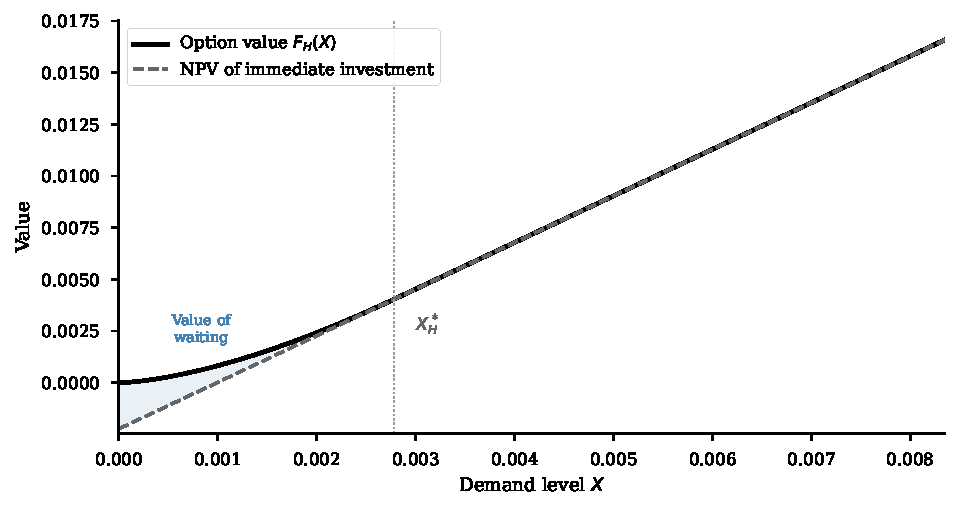
\includegraphics[keepaspectratio]{figures/fig_option_value.pdf}}

}

\caption{\label{fig-option-value}Option value versus NPV of immediate
investment in regime \(H\). The solid curve shows the option value
\(F_H(X)\); the dashed curve shows the NPV of investing immediately at
the trigger-optimal scale \(K_H^*\), held fixed across \(X\). The shaded
region is the ``value of waiting,'' the excess of the option value over
the NPV. The vertical dotted line marks the optimal trigger \(X_H^*\)
where smooth pasting holds. Parameters: baseline calibration
(\(\sigma = 0.25\), \(\mu_H = 0.06\), \(r = 0.12\), \(\alpha = 0.40\),
\(\gamma = 1.50\)).}

\end{figure}%

\textbf{Comparative statics of the H-regime policy.}
Figure~\ref{fig-comparative-statics} presents comparative statics for
the optimal trigger \(X_H^*\) and capacity \(K_H^*\) with respect to
four key parameters. Table~\ref{tbl-elasticities} reports elasticities
at the baseline for the full model's \(X^*\), \(K^*\), and \(\phi^*\),
which are not the H-regime objects plotted here. Panel (a) shows that
higher volatility \(\sigma\) raises both the trigger and the optimal
capacity: as in the full model (Internet Appendix C), uncertainty raises
the option value of waiting, so investment occurs at a higher demand
level, at which the optimal scale is larger. Panel (b) shows the effect
of revenue elasticity \(\alpha\): higher \(\alpha\) (less diminishing
returns) raises the trigger and substantially increases capacity, since
the marginal value of additional capacity is higher. Panel (c) shows
that greater cost convexity \(\gamma\) has a non-monotone effect on both
the trigger and the optimal capacity: \(K_H^*\) is \(0.0107\) at
\(\gamma = 1.20\), \(0.0034\) at \(1.35\), \(0.0067\) at \(1.50\), and
\(0.035\) at \(2.00\), with the trigger tracing a similar U-shape. With
the cost scale \(c\) held fixed, a higher exponent lowers the marginal
cost \(c\gamma K^{\gamma-1}\) for capacities below the normalized unit
\(K = 1\), where the optimum lies, once \(\gamma\) is large enough for
the exponent effect to dominate the factor \(\gamma\). Panel (d) shows
that higher operating cost \(\delta\) raises both the trigger and the
optimal capacity. As Internet Appendix C notes, this panel is a
rescaling of the capacity unit rather than an economic sensitivity. What
the panel does show is the role of the linear cost floor in creating the
interior optimum (Equation~\ref{eq-foc-K}).

\begin{figure}[!htb]

\centering{

\pandocbounded{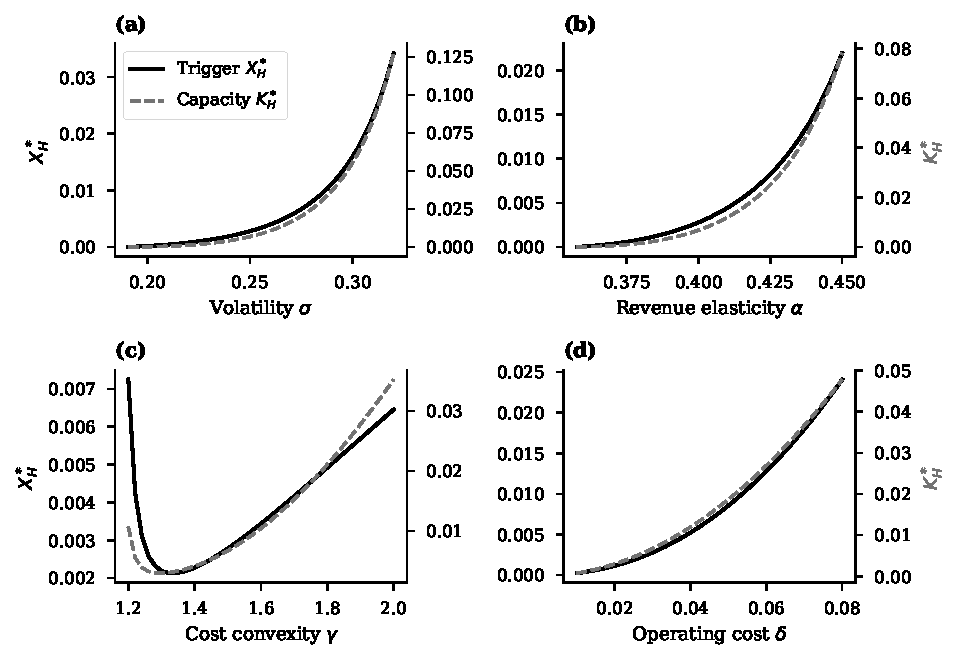
\includegraphics[keepaspectratio]{figures/fig_comparative_statics.pdf}}

}

\caption{\label{fig-comparative-statics}Comparative statics of the
single-firm investment policy in regime \(H\). Each panel varies one
parameter, holding the others fixed. Solid lines (left axis) show the
optimal trigger \(X_H^*\); dashed lines (right axis) show the optimal
capacity \(K_H^*\). (a) Volatility \(\sigma\); (b) revenue elasticity
\(\alpha\); (c) investment cost convexity \(\gamma\); (d) operating cost
rate \(\delta\). Parameters: baseline calibration.}

\end{figure}%

\newpage

\subsection*{G. A Normalized Scale-Gap
Diagnostic}\label{g.-a-normalized-scale-gap-diagnostic}
\addcontentsline{toc}{subsection}{G. A Normalized Scale-Gap Diagnostic}

Motivated by \citet{berk1999optimal}, this section asks how far a firm's
installed base sits from the model's optimal scale, and reports the
answer as a unit-free index; Section~\ref{sec-valuation} summarizes the
result. The scale-gap index \(g\) compares two quantities, defined
below: the value of the capacity already in place, and the shortfall of
that value relative to an optimally sized greenfield project. Expressing
the shortfall as a fraction of their sum puts the gap on a \([0, 1]\)
scale so that it can be read across calibrations.

The construction is deliberately \emph{not} a growth-option
decomposition. It does not measure the present value of future
investment opportunities, and the two quantities it compares are
benchmarks rather than separable claims on the firm: one is measured
gross of sunk investment cost, the other net of it. Their sum is
therefore a normalization device rather than a valuation identity, and
the resulting fraction is not a share of firm value or of market
capitalization. The object of interest is the \emph{shape} of the index
in \(K/K^*\), which is invariant to the cost normalization \(c = 1\)
(Section~\ref{sec-calibration}); its level at any particular point on
the horizontal axis is not.

The two components are the following.

\begin{enumerate}
\def\labelenumi{\arabic{enumi}.}
\item
  \textbf{Assets-in-place}: the value of existing installed capacity at
  current demand, incorporating both L-regime inference revenue and
  H-regime continuation value through \(A_{\text{eff}}\). \[
  V_{\text{AIP}} = A_{\text{eff}}(\phi, K_{\text{installed}}) \cdot X - \frac{\delta K_{\text{installed}}}{r}.
  \]
\item
  \textbf{Capacity gap value}: the shortfall of the current installed
  base relative to the optimally sized project, \[
  V_{\text{gap}} = \max\{\text{NPV}(K^*, \phi^*) - V_{\text{AIP}},\; 0\},
  \] where \(\text{NPV}(K^*, \phi^*)\) is the net (of the full
  investment cost \(I(K^*)\)) present value of the optimally sized
  greenfield project. This is a comparative-statics measure of distance
  to optimal scale, namely how far the firm's gross installed-asset
  value falls short of the net value of a full-scale deployment. It is
  not the NPV of incremental expansion from the installed base (which
  would credit the firm for capacity already sunk), and it is not a
  forward-looking option value. Because the benchmark nets out the
  entire investment cost while assets-in-place are gross of sunk costs,
  the gap reaches zero before \(K_{\text{installed}}\) reaches \(K^*\).
\end{enumerate}

The value of the possibility of transitioning from \(L\) to \(H\) does
not appear as a third additive term: it is embedded in \emph{both}
quantities through the effective revenue coefficient
\(A_{\text{eff}}(\phi, \cdot)\), which already weights the H-regime
continuation value by the arrival rate \(\lambda\) and the training
allocation \(\phi\). The scale-gap index is then \[
g(K_{\text{installed}}) = \frac{V_{\text{gap}}}{V_{\text{AIP}} + V_{\text{gap}}} \in [0, 1].
\]

Figure~\ref{fig-growth-decomposition} plots the index using the full
model with regime switching: values are computed with the effective
revenue coefficient \(A_{\text{eff}}\) at the optimal training fraction
\(\phi^*\), evaluated at demand \(1.5 X^*\). Panel (a) stacks
assets-in-place (blue, lower band) and the capacity gap (orange, upper
band) against installed capacity relative to the optimal level \(K^*\).
When the firm has little installed capacity (\(K/K^* \ll 1\)), the gap
dominates the stack; as installed capacity rises, assets-in-place
increase concavely (diminishing returns) while the gap shrinks. Panel
(b) plots \(g\), which falls from about 80\% at the left edge of the
figure (\(K/K^* = 0.01\)) to zero at \(K/K^* \approx 0.77\); the
crossover occurs where the gross value of installed assets overtakes the
optimal \emph{net} value, since assets-in-place are measured gross of
the sunk investment cost while the benchmark nets it out. At the
baseline calibration \(g\) equals 50\% at \(K/K^* = 0.1\) and 26\% at
\(K/K^* = 0.3\), so the index runs at roughly 25--50\% over that range;
the sweep in Internet Appendix E reports 48--59\% and 19--30\% at those
two points, so the band survives one-at-a-time perturbation of each
parameter by \(\pm 25\%\). Because \(c = 1\) fixes the cost scale by
normalization (Section~\ref{sec-calibration}), \(K^*\) is not a physical
quantity and \(K/K^*\) cannot be read off observed compute stocks; I
therefore make no claim about which point on the axis describes a given
firm, and the content of the figure is entirely the monotone decline and
the location of the crossover.

\begin{figure}[!htb]

\centering{

\pandocbounded{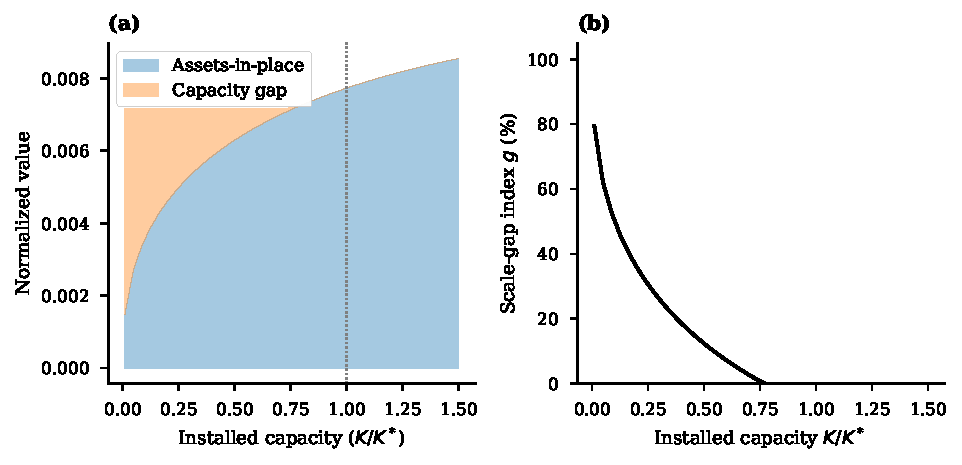
\includegraphics[keepaspectratio]{figures/fig_growth_decomposition.pdf}}

}

\caption{\label{fig-growth-decomposition}Normalized scale-gap
diagnostic. (a) Stacked plot of assets-in-place (blue, lower band) and
the capacity gap (orange, upper band) as a function of installed
capacity relative to the optimal level \(K^*\); the dotted line marks
\(K/K^* = 1\). (b) The scale-gap index
\(g = V_{\text{gap}}/(V_{\text{AIP}} + V_{\text{gap}})\) over the same
range, reaching zero at \(K/K^* \approx 0.77\). The two components are
measured against different benchmarks, one gross of sunk investment cost
and one net of it, so their sum is a normalization rather than a
valuation identity and \(g\) is not a share of firm value.
Horizontal-axis levels are not identified, because \(c = 1\) fixes the
cost scale by normalization. Parameters: full model with regime
switching at the optimal training fraction \(\phi^*\), demand at
\(1.5 X^*\), baseline calibration.}

\end{figure}%

The diagnostic carries no direct asset-pricing implication: the model
prices all claims by discounting at a single constant rate \(r\) and
contains no pricing kernel, so it cannot map a value composition into a
beta or an expected return. The related conjecture, that a larger
H-regime share of value raises equity betas, is stated in
Section~\ref{sec-discussion} as a hypothesis to be tested, not as a
result derived here.

\newpage

\subsection*{H. Credit Spreads and Default
Probabilities}\label{h.-credit-spreads-and-default-probabilities}
\addcontentsline{toc}{subsection}{H. Credit Spreads and Default
Probabilities}

The formulas and the leverage curves behind the credit-risk discussion
of Section~\ref{sec-valuation} are collected here.

\textbf{Credit spreads.} For a levered firm with leverage \(\ell\), the
credit spread is: \[
\text{spread} = \frac{C_D}{D(X)} - r,
\] where \(C_D = r_c \ell I(K)\) is the total coupon flow, \(D(X)\) is
the market value of debt given in Section~\ref{sec-model} (which differs
from face value because of default risk), and the reference rate is the
model's discount rate \(r\) (the WACC), not a risk-free rate.\footnote{The
  benchmark is the model's discount rate \(r\) because all claims are
  valued by discounting at \(r\): a default-free perpetuity with coupon
  \(C_D\) is worth \(C_D/r\) and yields exactly \(r\), so the spread is
  zero absent default risk and isolates the default-risk component. The
  model has a single, risk-adjusted discount rate and therefore cannot
  separately speak to the term-structure or risk-premium components of
  observed corporate spreads; the reported spreads are model-implied
  risk-adjusted objects, the default-risk increment over \(r\), and not
  market credit spreads or yield spreads over Treasuries.} The training
fraction \(\phi\) enters through \(A_{\text{eff}}\), which sets both the
default boundary \(X_D\) of Equation~\ref{eq-default-boundary} and the
liquidation value creditors recover there. Because leverage and the
coupon rate are exogenous stress-test parameters
(Section~\ref{sec-model}), the leverage gradients below describe the
model's response to an imposed debt burden, not an optimally chosen
capital structure. Higher leverage increases the default boundary
\(X_D\) and the coupon claim, reducing debt value and widening spreads.

\textbf{Default probability.} The probability of default within horizon
\(T\) is the first-passage probability for GBM hitting the barrier
\(X_D\): \[
P(\text{default within } T) = \mathcal{N}(-d_1) + \left(\frac{X_D}{X}\right)^{2\nu/\sigma^2} \mathcal{N}(-d_2),
\] where \(\nu = \mu_L - \sigma^2/2\),
\(d_1 = [\ln(X/X_D) + \nu T]/(\sigma\sqrt{T})\),
\(d_2 = [\ln(X/X_D) - \nu T]/(\sigma\sqrt{T})\), and \(\mathcal{N}\) is
the standard normal CDF. This is the exact barrier hitting probability
for GBM, consistent with the Leland-style first-passage default
mechanism in the model; the L-regime drift \(\mu_L\) is the relevant one
because the default boundary is an L-regime object (the firm defaults
pre-switch). The calculation abstracts from the regime switch itself,
since a switch to \(H\) before hitting \(X_D\) would effectively remove
default risk, so the reported figures are upper bounds on the pre-switch
default probability. Since \(\mu_L\) is the risk-adjusted
(certainty-equivalent) drift, the result is a \emph{model-implied
risk-adjusted} first-passage probability, computed under the same
convention as the spread calculation. It is not a risk-neutral
(pricing-measure) probability, because the model discounts at the WACC
rather than at a risk-free rate (see the footnote in
Section~\ref{sec-model}). The physical-measure probability, using the
unadjusted drift, would be lower.

\textbf{Leverage gradients.} Figure~\ref{fig-credit-risk} plots credit
spreads and default probabilities against leverage. Both panels are
evaluated at a fixed demand level \(X = 0.10\) for a firm with capacity
\(K = 1\) and training fraction \(\phi = 0.5\), a representative
interior allocation. Using the optimal \(\phi^* \approx 0.70\) instead
shifts the level of the curves modestly, through the two opposing
\(\phi\)-channels discussed in Section~\ref{sec-valuation}, without
changing their shape. At low leverage the spread is zero: the small
coupon claim is over-collateralized by the liquidation value of the
inference business, so debt is effectively riskless even though the
equity holders' default boundary is positive. Once the coupon claim
outgrows the inference collateral (around \(\ell \approx 0.13\) at the
evaluation point), the spread turns positive and rises with leverage,
reaching approximately 12 bps at \(\ell = 0.20\), 41 bps at
\(\ell = 0.40\), and 97 bps at \(\ell = 0.70\). Panel (b) shows the
model-implied risk-adjusted five-year default probability (first passage
under the risk-adjusted L-regime drift), which rises from 0.63\% at
\(\ell = 0.05\) to 1.80\%, 4.85\%, and 12.98\% at the same three
leverage levels. The steep increase in default probability at high
leverage reflects the shrinking distance to default: as leverage
increases, the default boundary \(X_D\) rises while the firm's demand
level is fixed, compressing the distance to default.

\begin{figure}[!htb]

\centering{

\pandocbounded{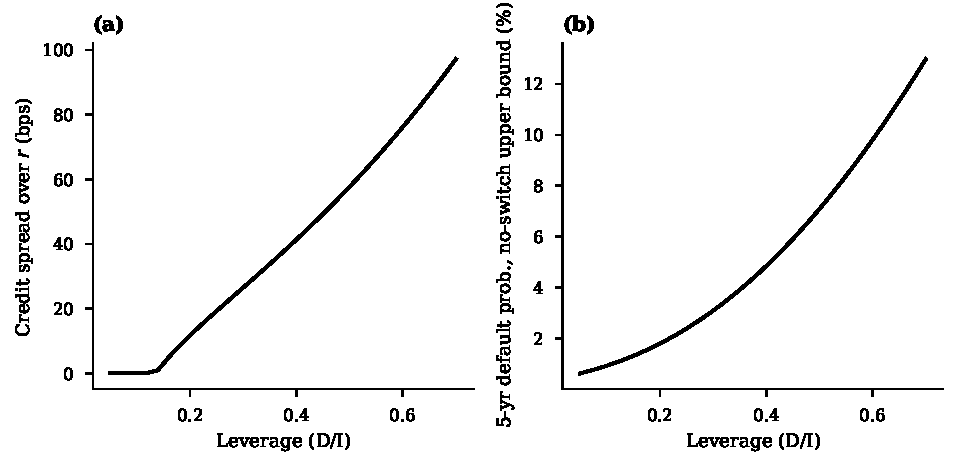
\includegraphics[keepaspectratio]{figures/fig_credit_risk.pdf}}

}

\caption{\label{fig-credit-risk}Credit risk as a function of leverage.
(a) Credit spread in basis points, measured relative to the model's
discount rate \(r\) rather than a risk-free rate. (b) Model-implied
risk-adjusted five-year default probability (first passage under the
risk-adjusted L-regime drift, with the regime switch omitted, so an
upper bound on the pre-switch probability). Neither panel reports a
risk-neutral (pricing-measure) object nor a market credit spread.
Evaluated at a fixed demand level \(X = 0.10\) with capacity \(K = 1\)
and training fraction \(\phi = 0.5\), using the Leland structural model
with exogenous leverage, a stylized coupon rate \(r_c = 0.05\), and
bankruptcy cost \(b = 0.30\). Parameters: baseline calibration.}

\end{figure}%

\newpage

\subsection*{I. Supplementary Literature and
Motivation}\label{i.-supplementary-literature-and-motivation}
\addcontentsline{toc}{subsection}{I. Supplementary Literature and
Motivation}

This section collects empirical motivation and literature detail that
supported earlier drafts of Section~\ref{sec-introduction} and
Section~\ref{sec-literature} but was cut to hold the main text near the
target length; it does not introduce new results.

\textbf{Duopoly as the strategic setting.} Section~\ref{sec-model} fixes
duopoly as the strategic environment; the choice is motivated
empirically. Frontier AI training competition is concentrated: on public
accounts, the largest training runs to date have been conducted by a
handful of laboratories, often backed by or partnered with a single
cloud provider (e.g., Anthropic--Amazon, OpenAI--Microsoft) or building
proprietary clusters (e.g., xAI's Colossus). The dominant strategic
margin is therefore not atomistic competition but rivalry among a few
labs, each making multi-billion-dollar capacity commitments, and duopoly
is the minimal model that captures the resulting forces, strategic
preemption, race-like training-allocation incentives, and
continuation-value effects under leverage, while keeping the closed-form
characterization tractable.\footnote{An \(N>2\) extension along the
  lines of \citet{bouis2009multistage} may be feasible but would
  sacrifice the closed-form characterization that makes the duopoly
  results transparent.}

\textbf{A modeling caveat on the capacity variable.} The capacity
variable \(K\) in Section~\ref{sec-model} is a reduced form for the AI
infrastructure investment bundle, not solely for compute
hardware.\footnote{In practice, AI infrastructure investment also
  encompasses substantial expenditure on power generation and
  transmission (dedicated natural gas plants, long-term power purchase
  agreements, on-site substations) required to supply the hundreds of
  megawatts that a single training cluster demands. For tractability,
  the model treats all of these complementary investments as a single
  capital outlay in ``compute capacity,'' with the cost function
  \(I(K) = cK^\gamma\) absorbing the full cost of bringing a unit of
  capacity online, including its power supply.}

\textbf{Annotated literature note.} The paragraphs below extend the
discussion in Section~\ref{sec-literature} with additional antecedents
and detail that did not fit the space constraint of the main text.

\emph{Real options and capacity choice.} Beyond the timing foundations
in \citet{mcdonald1986value} and \citet{pindyck1988irreversible}, other
foundational contributions include \citet{brennan1985evaluating} and
\citet{bernanke1983irreversibility}. The capacity-choice problem is also
the subject of a large operations management literature surveyed by
\citet{vanmieghem2003capacity}; its closest construct, resource
flexibility, is developed by \citet{chod2005resource}, who show that a
flexible resource allocated across products \emph{after} demand is
observed substitutes for capacity and interacts with pricing. On the
strategic side, \citet{weeds2002strategic} study R\&D delay under a
real-options framework and \citet{fudenberg1985preemption} supply the
game-theoretic foundations for preemption.
\citet{aguerrevere2003equilibrium} shows that operating flexibility can
make firms \emph{expand}, rather than contract, in response to greater
uncertainty, and \citet{aguerrevere2009real} draws out the asset-pricing
implication that installed capacity and competitive intensity jointly
determine the composition of firm value between assets in place and
growth options, and hence expected returns; here the risk composition
shifts with the \emph{split} of a given capacity rather than with its
level. The paper's emphasis on heterogeneous beliefs about the arrival
rate \(\lambda\) connects to the literature on disagreement and
speculation
\citep{harrison1978speculative, scheinkman2003overconfidence}, though
here disagreement enters through comparative statics in \(\lambda\)
rather than through equilibrium trading under heterogeneous priors.
\citet{grenadier2011real} develop real-options signaling games in which
investment timing conveys private information, which bears on the
dynamic belief updating raised as a future direction in
Section~\ref{sec-conclusion}, and \citet{bouis2009multistage} provide an
\(N\)-firm sequential-entry framework that could extend the duopoly
analysis of this appendix and of Section~\ref{sec-model}.

\emph{R\&D races.} \citet{loury1979market} models firms choosing R\&D
intensity to accelerate a stochastic Poisson breakthrough, showing that
competition leads to socially excessive duplication of effort, and
\citet{reinganum1982strategic} extends the framework to asymmetric
firms, showing that the frontrunner invests more aggressively; the
parallel with the leader's earlier entry in the preemption equilibrium
of Proposition 3 is loose, because Reinganum's frontrunner is defined by
its technological position, whereas here the leader's role is itself an
outcome of the timing game. \citet{harris1987racing} model R\&D as a
race with position-dependent investment incentives, producing a
discouragement effect for lagging firms, and \citet{grossman1986optimal}
study simultaneous timing and scale choices in R\&D competition under
uncertainty, combining elements of the capacity and timing decisions
modeled here.

\emph{Structural credit risk.} \citet{blackcox1976valuing} extend the
Merton framework to a first-passage setting.
\citet{hackbarth2006capital} let cash flows depend on a two-state
macroeconomic regime and derive default and financing policies that
adapt to the cycle, reproducing countercyclical leverage ratios and
strictly positive short-maturity credit spreads;
\citet{chen2010macroeconomic} and \citet{bhamra2010levered} add a
consumption-based pricing kernel, so that risk prices, leverage, and
regime-contingent default boundaries are determined jointly. That
regime-switching literature makes the default boundary depend on the
state, but the regime governs the cash-flow process exogenously, so the
size of the growth option is not a decision variable and cannot be
traded off against current cash flow; here the firm chooses the training
fraction \(\phi\), and that choice determines both the regime-\(H\)
continuation value and the regime-\(L\) coupon coverage, which is why
the default boundary can be \emph{decreasing} in the training fraction
(\textbf{?@eq-phi-underbar}). The most closely related papers combining
investment and default are \citet{hackbarth2014capital}, who study real
options with endogenous default and product-market competition, and
\citet{kumar2018optimal}, who show that joint leverage and irreversible
capacity choice are substitutes; \citet{sundaresan2015dynamic} model
growth options with default risk and \citet{bolton2019investment} model
financial constraints on investment. The present model builds on
\citet{hackbarth2012corporate} for the investment-financing framework
and integrates endogenous default into the strategic capacity-choice
game.

\emph{Economics of AI.} \citet{jones1995rdbased} and
\citet{bloom2020ideas} study diminishing returns in idea production.
\citet{babina2024artificial} and \citet{eisfeldt2023generative} provide
empirical context on AI investment and valuations; these papers could in
principle discipline certain calibration inputs (e.g., AI firm betas,
investment intensities), though the rapidly evolving nature of the
sector limits the stability of such inputs. The Baumol mechanism in
\citet{aghion2019artificial}, under which growth is limited by the tasks
that remain essential and hard to automate, plays a role loosely
analogous to the diminishing returns \(\alpha < 1\) imposed at the firm
level here; the present paper is partial equilibrium and therefore
complements these general-equilibrium analyses by providing a
micro-founded model of the firm-level investment and allocation
decisions that aggregate into the industry dynamics those papers study.
\citet{novymarx2007operating} shows that operating leverage amplifies
systematic risk, relevant to the operating cost parameter \(\delta\).

\emph{Marginal contribution, restated.} Each adjacent literature is
missing one ingredient of the mechanism at the center of the paper: the
models that combine capacity choice with endogenous default
\citep{hackbarth2014capital, kumar2018optimal} treat installed capital
as homogeneous, so there is no split to choose; the regime-switching
credit models
\citep{hackbarth2006capital, chen2010macroeconomic, bhamra2010levered}
take the cash-flow process, and with it the size of the growth option,
as exogenous; and the allocation problems closest in structure
\citep{akcigit2018growth, chod2005resource} are solved for firms whose
survival is not at stake. The contribution is the joint presence of the
three, not any one of them.





\end{document}
